\documentclass[12pt,a4paper,openany,oneside]{book}

\usepackage{hyperref}
\usepackage[italian]{babel}

\usepackage[utf8x]{inputenc}
\usepackage[T1]{fontenc}

\usepackage{graphicx}
\usepackage[font=small,labelfont=bf,tableposition=top]{caption}

\usepackage[headheight=12pt, textheight=592pt, marginparsep=7pt, footskip=30pt, hoffset=0pt, paperwidth=597pt,
            top=127pt, headsep=19pt, textwidth=390pt, marginparwidth=38pt, voffset=0pt, paperheight=845pt,
            left=117pt, right=90pt]{geometry} % Metto un margine più largo a sinistra per la rilegatura
\usepackage{listings}
\usepackage{inconsolata}
\usepackage{xcolor}
\usepackage[framemethod=tikz]{mdframed}

\definecolor{commentsgreen}{rgb}{0, 0.6, 0} % Per i commenti
\definecolor{codegray}{rgb}{0.5, 0.5, 0.5} % Per i numeri di riga
\definecolor{keywordpurple}{rgb}{0.77, 0.525, 0.75} % Per le keyword
\definecolor{backcolour}{rgb}{0.12, 0.12, 0.12} % Colore grigio scuro per lo sfondo
\definecolor{functionyellow}{rgb}{0.86, 0.86, 0.667} % Colore blu per le tue funzioni
\definecolor{basicblue}{rgb}{0.61, 0.86, 1} % Colore blu per il testo
\definecolor{classgreen}{rgb}{0.294, 0.745, 0.6} % Colore verde per le classi
\definecolor{numberyellow}{rgb}{0.686, 0.705, 0.435} % Colore giallo per i numeri
\definecolor{stringbrown}{rgb}{0.8, 0.51, 0.298} % Colore marrone per le stringhe
\definecolor{defblue}{rgb}{0.2, 0.32, 0.833} % Colore blu per le definizioni
\definecolor{constantblue}{rgb}{0.2, 0.705, 1} % Colore blu per le costanti

\lstset{
        language=Python,
        basicstyle=\footnotesize\ttfamily\color{basicblue},
        numbers=left,
        numberstyle=\tiny\ttfamily\color{codegray},
        numbersep=8pt,
        tabsize=5,
        escapeinside={(*@}{@*)},
        extendedchars=true,
        breaklines=true,
        backgroundcolor=\color{backcolour},
        commentstyle=\ttfamily\color{commentsgreen},
        keywordstyle=\ttfamily\color{keywordpurple},
        deletekeywords={print, dict, all, list, str},
        stringstyle=\ttfamily\color{stringbrown},
        showspaces=false,
        showtabs=false,
        xleftmargin=17pt,
        framexleftmargin=17pt,
        framexrightmargin=5pt,
        framexbottommargin=4pt,
        showstringspaces=false,
        captionpos=b,
        morekeywords=[2]{load_from_local, get_vectors, get_labels, fit_transform, from_pretrained, to, generate, decode, print, load, split_documents, from_documents, as_retriever, format_docs, join, invoke, from_template, batch, make, __init__, add_documents, append, create_chunks, save_local, load_config, load_dotenv, find_dotenv, add_dir, get_data, test, add, is_available, embed_query, create_history_aware_retriever, create_retrieval_chain, create_stuff_documents_chain, from_messages, _get_relevant_documents, get_child, compress_documents, filter_by_similarity, search_by_vector, get},
        keywordstyle=[2]\ttfamily\color{functionyellow},  % Stile per le funzioni
        morekeywords=[3]{sklearn, manifold, TSNE, preprocessing, LabelEncoder, vectordb, VectorDatabase, transformers, AutoTokenizer, AutoModelForCausalLM, torch, WebBaseLoader, langchain_community, langchain_core, langchain, document_loaders, text_splitter, bs4, RecursiveCharacterTextSplitter, dict, SoupStrainer, langchain_huggingface, HuggingFaceEmbeddings, vectorstores, Chroma, prompts, output_parsers, runnables, RunnablePassthrough, StrOutputParser, PromptTemplate, langchain_ollama, OllamaLLM, data_manager, Data, Splitter, FAISS, tqdm, DBMaker, docstore, InMemoryDocstore, DataList, utilities, dotenv, faiss, IndexFlatL2, chains,history_aware_retriever, RunnableWithMessageHistory, ChatPromptTemplate, MessagesPlaceholder, history, llms, retrieval, combine_documents, Document, CallbackManagerForRetrieverRun},
        keywordstyle=[3]\ttfamily\color{classgreen},  % Stile per le classi
        morekeywords=[4]{RAG_PROMPT, TRANSFORM_PROMPT},
        keywordstyle=[4]\ttfamily\color{constantblue},  % Stile per le costanti
        literate={.}{{\textcolor{white}{.}}}1 
                 {=}{{\textcolor{white}{=}}}1
                 {,}{{\textcolor{white}{,}}}1
                 {:}{{\textcolor{white}{:}}}1
                 {|}{{\textcolor{white}{|}}}1
                 {+}{{\textcolor{white}{+}}}1
                 {-}{{\textcolor{white}{-}}}1
                 {>}{{\textcolor{white}{>}}}1
                 {<}{{\textcolor{white}{<}}}1
                 {*}{{\textcolor{white}{*}}}1
}
 
% Questo serve per cambiare il nome della lista dei codici in "Codice"
\addto\captionsitalian{
        \renewcommand{\lstlistingname}{Codice}}

% Questo pacchetto serve per inserire e numerare le subsection
\setcounter{tocdepth}{2} % numerazione indice
\setcounter{secnumdepth}{2} % numerazione nel testo

\usepackage{amsmath}
\usepackage{amssymb}
\usepackage{float}
\usepackage{framed}
\usepackage{layout} % Per visualizzare il layout della pagina

\begin{document}

\newgeometry{top=2.5cm, bottom=3cm, left=2.5cm, right=2.5cm}
\begin{titlepage}
\centering 


\includegraphics[width=3.5cm,height=3.5cm]{Images/svg_logo.pdf}

\bigskip

\bigskip

\bigskip % metto 3 skip dopo il logo dell'università

{\Large \textbf{UNIVERSIT\`A DEGLI STUDI DI CATANIA}}

{\scshape
\large
Dipartimento di Matematica e Informatica
}

{\scshape
\normalsize
Corso di Laurea Triennale in Informatica
}

\bigskip % metto 1 skip dopo la descrizione del corso di laurea

\hrule % faccio una riga orizzontale

\bigskip

\bigskip

\bigskip

\bigskip

\bigskip % metto 5 skip dopo la riga orizzontale

{\itshape
\large
Giuseppe Cosimo Alfio Bellamacina
\par}

\bigskip

\bigskip

\bigskip

\bigskip

\bigskip % metto 5 skip dopo il mio nome

{\centering
\Large
Dalla Ricerca alla Risposta: \\
Il Nuovo Paradigma Conversazionale \\
grazie all'Intelligenza Artificiale
\par}

\bigskip

\bigskip

\bigskip

\bigskip

\bigskip

\bigskip % metto 6 skip dopo il titolo della tesi

\begin{minipage}[b]{8 cm} % faccio una minipage per una riga più stretta
\hrule

\bigskip

{\centering\scshape 
Relazione Progetto Finale
\par}

\bigskip

\hrule
\end{minipage} % chiudo la minipage

\bigskip

\bigskip

\bigskip

\bigskip

\bigskip

\bigskip

\bigskip

\bigskip

\bigskip

\bigskip

\bigskip % metto 11 skip dopo la riga orizzontale

\vspace*{\fill}

\begin{flushright}
    \begin{tabular}{@{}l}
    Relatore: \\
    Chiar.mo Prof. Sebastiano Battiato \\
    \\
    Correlatore: \\
    Dott. Ing. Mario Barbera
    \end{tabular}
\end{flushright}

\bigskip

\bigskip

\bigskip

\bigskip % metto 4 skip dopo i nomi del relatore e del correlatore

\hrule

\bigskip

{\centering
Anno Accademico 2023 - 2024
\par}
\end{titlepage}

\restoregeometry

\chapter*{Abstract}
Lo sviluppo di tecnologie all'avanguardia ha trasformato profondamente le nostre vite. Negli ultimi anni, l'avanzamento esponenziale nelle tecniche di produzione di componenti hardware e nell'elaborazione di algoritmi di apprendimento automatico sempre più efficienti, ha favorito una rapida evoluzione nel campo del Machine Learning e del Deep Learning.
Di particolare interesse è il modo in cui queste tecnologie si interfacciano con il mondo del Natural Language Processing (NLP), e come questo approccio apra a possibilità quasi infinite. I Large Language Models (LLM), basati sull'architettura Transformer, hanno rivoluzionato il modo in cui le macchine comprendono e generano il linguaggio naturale, in più, l'integrazione con tecniche di Retrieval-Augmented Generation (RAG) ha ampliato ulteriormente le capacità e conoscenze di questi modelli, consentendo di combinare la generazione di linguaggio con il recupero di informazioni rilevanti da dataset estesi, rendendoli più applicabili a una vasta gamma di compiti.
Questa tesi non solo analizza le principali architetture alla base di questi modelli ma ne mostra molte delle loro applicazioni pratiche, mettendo in luce sia i punti di forza sia i loro lati oscuri. Inoltre, presenta una sperimentazione pratica attraverso lo sviluppo di un chatbot, "OmniBot", che implementa l'architettura RAG all'interno di una catena di pensiero personalizzata, denominata “Chain-of-Thoughts” (CoT). Verranno analizzati tutti i passi che hanno portato alla realizzazione di questo prototipo e verrà mostrato come questo approccio, oltre a migliorare la coerenza e la pertinenza delle risposte generate, può anche stabilire limitazioni mirate al comportamento del modello quando necessario, dimostrando, dunque, l'efficacia delle soluzioni discusse.
Infine, verranno presentati i risultati ottenuti attraverso test empirici e verranno discusse le possibili evoluzioni future di questo progetto.

\tableofcontents

\chapter*{Introduzione}
\markboth{\MakeUppercase{Introduzione}}{\MakeUppercase{Introduzione}}
\addcontentsline{toc}{chapter}{Introduzione}
Lo sviluppo di tecnologie avanzate nel campo dell'apprendimento automatico ha portato a cambiamenti radicali nel modo in cui i sistemi intelligenti interagiscono con il mondo circostante. In questa tesi verrà trattata inizialmente la teoria alla base dei Large Language Models (LLM), analizzando le principali tappe che hanno portato alla loro evoluzione. Si esamineranno alcuni dei modelli predecessori, evidenziando le sfide affrontate e le soluzioni trovate per superare i loro limiti. Questi modelli, pur rappresentando importanti passi avanti, presentavano difficoltà significative nel gestire contesti complessi e nel catturare dipendenze linguistiche a lungo raggio, problemi che sono stati in gran parte risolti con l'introduzione del modello Transformer.

Quest'ultimo, grazie al suo innovativo meccanismo di attenzione, ha portato ad una rivoluzione nel campo del Natural Language Processing (NLP) poiché consente di catturare con grande precisione le dipendenze tra le parole, anche quando queste sono distanti all'interno di una frase. Questo ha consentito di superare i limiti strutturali dei modelli precedenti, come le reti ricorrenti, e ha gettato le basi per la creazione di modelli linguistici di dimensioni e capacità senza precedenti, i cosiddetti Large Language Models.

Tuttavia, nonostante la potenza degli LLM, essi presentano ancora una limitazione fondamentale: il loro apprendimento si basa su grandi quantità di dati statici, e non sono in grado di aggiornare o acquisire nuove informazioni in modo dinamico senza essere riaddestrati. Per rispondere a questa sfida, è stata introdotta una tecnica innovativa, la Retrieval-Augmented Generation (RAG), che ottimizza il processo di accesso alle informazioni. A differenza dei metodi tradizionali, che richiedono ai modelli di memorizzare tutto ciò che hanno appreso, la RAG sfrutta un database esterno per recuperare in tempo reale le informazioni necessarie. Si elimina il bisogno di fornire un apprendimento continuo al modello stesso. Questa tecnica non solo rende i modelli più efficienti e scalabili, ma permette loro di essere aggiornati e personalizzati in modo dinamico e veloce.

Dopo aver discusso le teorie alla base di questi concetti, la tesi si concentrerà su un'applicazione pratica concreta: lo sviluppo di un chatbot chiamato "OmniBot", nato a partire da un progetto assegnato durante un tirocinio curriculare presso l'azienda Intellisync \cite{intellisync}, basato sull'integrazione dell'architettura RAG all'interno di una catena di pensiero personalizzata, nota come "Chain-of-Thoughts" (CoT). Verranno analizzate dettagliatamente tutte le fasi del processo di sviluppo, dai primi esperimenti fino alla creazione del prototipo finale. Ogni passaggio del processo evolutivo sarà esplorato, mettendo in relazione gli accorgimenti progettuali adottati con le difficoltà che li hanno resi necessari e come le soluzioni scelte per affrontare i problemi riscontrati abbiano contribuito a migliorare il sistema complessivo.

L'implementazione di OmniBot rappresenta non solo una dimostrazione pratica dell'efficacia della RAG e della CoT, ma anche un'approfondita indagine su come queste tecnologie possano essere combinate per migliorare significativamente la coerenza, la pertinenza e l'accuratezza delle risposte generate dal chatbot. In particolare, verrà illustrato come l'integrazione di un database esterno con una struttura di ragionamento basata sulla catena di pensiero consenta di gestire in modo dinamico il recupero delle informazioni, mantenendo al contempo un controllo mirato sul comportamento del modello. Questo approccio garantisce una maggiore flessibilità e adattabilità rispetto ai modelli tradizionali e permette una gestione più precisa delle risposte in base al contesto e agli obiettivi prefissati.

Oltre alla descrizione tecnica, la tesi si concentrerà anche sull'analisi critica dei risultati ottenuti. Verranno presentati i dati emersi dai test sperimentali condotti su OmniBot, con l'obiettivo di dimostrare come l'approccio combinato di RAG e CoT possa essere applicato efficacemente in contesti reali, migliorando l'esperienza dell'utente e ottimizzando le performance del sistema. Le sperimentazioni non solo confermeranno la validità teorica del modello, ma forniranno anche indicazioni preziose su possibili miglioramenti futuri, mettendo in luce le aree in cui sono necessari ulteriori sviluppi o adattamenti.

Infine, la tesi esplorerà le potenziali evoluzioni di queste tecnologie, proiettandosi verso il futuro delle architetture di LLM potenziate. Verranno analizzate le sfide ancora aperte, come l'incremento della capacità di gestione di contesti ancora più complessi o l'introduzione di meccanismi avanzati di supervisione, così come le opportunità che potrebbero emergere con l'integrazione di tecniche di ottimizzazione più sofisticate. Le conclusioni indicheranno non solo i miglioramenti concreti raggiunti nel corso del progetto, ma anche le direzioni in cui queste tecnologie potranno evolversi, contribuendo ulteriormente all'avanzamento del campo dell'NLP.

\chapter{Large Language Models}
Quando si parla di Large Language Models (LLM) \cite{minaee2024largelanguagemodelssurvey}, si fa riferimento a modelli di deep learning, quindi basati su reti neurali profonde, progettati per elaborare dati non strutturati, in particolare il testo, in linguaggio naturale. Questi modelli, addestrati su enormi quantità di dati testuali, sono in grado di comprendere il contesto ricevuto, generare testi coerenti e rispondere a input linguistici in modo accurato. Alcuni modelli avanzati sono anche in grado di gestire contenuti multimediali, come audio, immagini e video, attraverso estensioni multimodali, sebbene la loro competenza primaria riguardi la comprensione e generazione del linguaggio naturale.

\section{Le origini}
Analizziamo prima le origini degli LLM e i principali sviluppi che hanno portato alla creazione di modelli sempre più avanzati e performanti.

\subsection{Modelli di linguaggio tradizionali}
Prima dell'introduzione delle reti neurali, i modelli di linguaggio si basavano principalmente su approcci statistici. Questi metodi erano utili per stimare la probabilità di una parola in una sequenza, ma avevano limitazioni significative nella capacità di catturare le dipendenze a lungo raggio e le complessità semantiche e sintattiche del linguaggio naturale.
\begin{itemize}
	\item \textbf{Modelli N-gramma}: Questi modelli stimano la probabilità di una parola in base alle \(N - 1\) parole precedenti. Ad esempio, un modello bigramma (\(N = 2\)) calcola la probabilità di una parola basandosi solo sulla parola immediatamente precedente, mentre uno trigramma (\(N = 3\)) considera le due parole precedenti. Gli N-grammi sono stati ampiamente utilizzati per la traduzione automatica e il riconoscimento del parlato, ma soffrono di alcuni problemi:
	\begin{itemize}
		\item \textbf{Sparsità dei dati}: Più aumenta il valore di \(N\), più diventa difficile raccogliere abbastanza dati per coprire tutte le possibili sequenze di \(N\) parole. Questo porta a un problema di sparsità, dove molte combinazioni di parole non sono mai state osservate durante l'addestramento.
		\item \textbf{Dipendenze a lungo raggio}: Gli N-grammi non possono catturare relazioni a lungo raggio tra le parole. Ad esempio, in una frase complessa, parole che appaiono molto distanti possono essere fortemente correlate, ma un modello N-gramma con un \(N\) basso non sarà in grado di cogliere questa relazione.
	\end{itemize}
	\item \textbf{Modelli a Catena di Markov}: I modelli di Markov, come gli N-grammi, ipotizzano che la probabilità di utilizzo di una parola dipenda solo da un numero limitato di parole precedenti. Nelle catene di Markov di ordine \(k\), la probabilità di una parola viene calcolata in base alle \(k\) parole precedenti. Questi modelli sono molto simili agli N-gramma e condividono molte delle stesse limitazioni. Una variante di questi modelli, le Hidden Markov Models (HMM) \cite{stolcke1994bestfirstmodelmerginghidden}, sono state ampiamente utilizzate per compiti come il riconoscimento del parlato e il part-of-speech tagging, dove lo stato latente rappresenta informazioni nascoste (ad esempio, la parte del discorso) che generano l'output osservato (la parola).
	\item \textbf{Modelli di Massima Entropia (MaxEnt)}: Questi modelli fanno uso di informazioni contestuali multiple (feature) per stimare la probabilità di una parola, massimizzando l'entropia soggetta a vincoli. I modelli di massima entropia non fanno assunzioni forti sul contesto e possono combinare diverse fonti di informazione per fare previsioni, ma anch'essi sono limitati quando si tratta di catturare relazioni a lungo termine nel testo.
	\item \textbf{Modelli di Interpolazione e Smoothing}: Per mitigare il problema della sparsità nei modelli N-gramma, vennero introdotte tecniche di smoothing come Laplace smoothing o Kneser-Ney smoothing, che assegnano probabilità non nulle anche a sequenze di parole mai osservate. Anche tecniche di interpolazione sono state sviluppate per combinare modelli N-gramma di diversi ordini, migliorando così la robustezza.
\end{itemize}
Questi modelli, pur essendo stati pionieristici e molto utilizzati, avevano una comprensione limitata del linguaggio. Erano rigidi nella loro capacità di generalizzare, poiché dipendevano da pattern ripetitivi che non potevano adattarsi facilmente a frasi complesse o nuove combinazioni di parole. Questo ha spianato la strada all'introduzione di approcci più avanzati, come le reti neurali ricorrenti (RNN), che potevano superare queste limitazioni catturando relazioni più complesse tra le parole e gestendo dipendenze a lungo raggio.

\subsection{Recurrent Neural Networks}
Negli anni '90 e 2000, l'avvento delle Recurrent Neural Networks (RNN) ha segnato un importante passo avanti nel campo del Natural Language Processing. A differenza dei modelli tradizionali, le RNN sono state progettate per gestire dati sequenziali, permettendo alla rete di avere una memoria interna che si aggiorna ad ogni passo temporale. Questa capacità di elaborare input di lunghezza variabile ha reso le RNN particolarmente adatte per attività come la traduzione automatica, il riconoscimento del parlato e la generazione di testo, dove il contesto a lungo termine gioca un ruolo cruciale.
Le RNN, in teoria, possono modellare le dipendenze temporali tra elementi in una sequenza, poiché ogni neurone dell'RNN riceve non solo l'input corrente ma anche l'output del passo precedente. Questo crea un meccanismo di feedback che consente alla rete di "ricordare" informazioni di stati passati e di propagare queste informazioni attraverso la rete per più passaggi temporali.

\subsubsection{Architettura delle RNN}
La struttura base di una RNN consiste in una serie di layer ricorrenti che prendono in input una sequenza temporale di dati e calcolano uno stato nascosto ad ogni passo temporale. Questo stato nascosto viene poi utilizzato come input per il passo successivo, insieme al nuovo dato della sequenza. La ricorrenza nella rete permette di mantenere una "memoria" delle informazioni passate, e tale informazione può essere utilizzata per prendere decisioni basate sul contesto storico del testo. Nelle applicazioni NLP, questo significa che ogni parola nella sequenza può influenzare le previsioni delle parole successive.

\subsubsection{Problema del Vanishing Gradient}
Per quanto le RNN abbiano portato una grande innovazione, questi modelli soffrivano di un problema noto come Vanishing Gradient. Questo fenomeno si verifica durante la fase di addestramento, quando si utilizzano tecniche di ottimizzazione basate su gradienti, come la Backpropagation Through Time (BPTT). Con l'aumentare della lunghezza delle sequenze, i gradienti calcolati per aggiornare i pesi della rete tendevano a diminuire esponenzialmente, rendendo difficile l'aggiornamento dei parametri dei layer ricorrenti. Di conseguenza, le RNN faticavano ad apprendere dipendenze a lungo termine tra parole o frasi distanti all'interno di un testo, limitando la loro capacità di comprendere il contesto globale in una sequenza lunga.

\subsubsection{Problema dell'Exploding Gradient}
In contrasto con il problema del vanishing gradient, a volte si osservava anche un fenomeno opposto noto come Exploding Gradient, in cui i gradienti crescevano esponenzialmente durante l'addestramento, causando instabilità nei processi di ottimizzazione. Questo fenomeno richiedeva l'uso di tecniche di regolazione, come il Gradient Clipping, per evitare che i gradienti esplodessero durante la retropropagazione.

\subsubsection{Applicazioni delle RNN}
Nonostante questi problemi, le RNN sono state adottate con successo in vari campi del NLP. Esse erano particolarmente adatte per applicazioni come:
\begin{itemize}
	\item \textbf{Traduzione automatica}: Dove la sequenza di parole in una lingua veniva mappata in una sequenza di parole in un'altra lingua.
	\item \textbf{Riconoscimento del parlato}: Si riconoscono parole e frasi a partire da segnali audio, grazie alla capacità delle reti di modellare le dipendenze temporali nei dati acustici.
	\item \textbf{Generazione di testo}: Le RNN potevano generare sequenze di testo una parola alla volta, tenendo conto del contesto delle parole precedenti.
\end{itemize}

\subsection{Gated Recurrent Neural Networks}
Una delle principali limitazioni delle Recurrent Neural Networks (RNN) tradizionali, ovvero la difficoltà nel catturare le dipendenze a lungo termine, è stata mitigata con l'introduzione delle Gated Recurrent Neural Networks (GRNN). Questi modelli rappresentano una famiglia di RNN che integrano meccanismi di gating, i quali, permettono alla rete di controllare in modo più efficiente il flusso delle informazioni, consentendo così alla stessa di decidere quali informazioni mantenere, aggiornare o dimenticare nel corso dell'elaborazione di una sequenza. Questo approccio consente di gestire con maggiore efficacia i problemi associati al vanishing gradient e all'incapacità di modellare sequenze lunghe.
Le due implementazioni più popolari di Gated RNN sono le Long Short-Term Memory (LSTM) e le Gated Recurrent Units (GRU), che hanno dimostrato una straordinaria efficacia in molte applicazioni di NLP e apprendimento sequenziale.

\subsubsection{Long Short-Term Memory (LSTM)}
Le Long Short-Term Memory \cite{10.1162/neco.1997.9.8.1735,sak2014longshorttermmemorybased,cheng2016longshorttermmemorynetworksmachine}, proposte da Hochreiter e Schmidhuber nel 1997, sono state progettate appositamente per affrontare le limitazioni delle RNN classiche. Esse sono costituite da una struttura più complessa rispetto alle RNN standard, con l'inclusione di una cella di memoria interna e tre principali gate (o porte), che regolano il flusso delle informazioni all'interno della rete. Questi gate consentono alla rete di conservare informazioni per periodi di tempo più lunghi e di decidere quali dati devono essere eliminati, quali devono essere aggiornati e quali devono essere trasmessi all'output. Essi sono:
\begin{itemize}
	\item \textbf{Input Gate}: Questo gate decide quali nuove informazioni devono essere aggiunte alla cella di memoria. L'input gate prende in input il nuovo dato e lo combina con lo stato precedente della cella di memoria, determinando quali informazioni aggiornare.
	\item \textbf{Forget Gate}: È il gate che controlla quali informazioni della cella di memoria devono essere eliminate o mantenute. Il forget gate è essenziale per evitare che la cella di memoria si riempia di informazioni obsolete o irrilevanti, permettendo alla rete di "dimenticare" informazioni non necessarie.
	\item \textbf{Output Gate}: Il gate di output stabilisce quale parte della cella di memoria deve essere utilizzata per generare l'output corrente. Questo processo è cruciale per garantire che l'output sia basato non solo sull'input attuale, ma anche su un contesto ben regolato dalle informazioni memorizzate in precedenza.
\end{itemize}
L'aggiunta di questi gate permette alle LSTM di catturare dipendenze a lungo termine all'interno di sequenze, risolvendo il problema delle sequenze estese e migliorando significativamente le prestazioni in compiti come la traduzione automatica, il riconoscimento del parlato e la generazione di testo.

\paragraph{Vantaggi delle LSTM}
Sono particolarmente potenti quando si tratta di modellare sequenze lunghe e complesse. La loro capacità di mantenere una memoria controllata, attraverso i gate, permette di evitare la perdita di informazioni critiche durante l'elaborazione delle sequenze, il che le rende adatte per:
\begin{itemize}
	\item \textbf{Predizione di serie temporali}: dove la rete deve tenere conto di eventi molto distanti nel tempo.
	\item \textbf{Traduzione automatica}: in cui la comprensione di frasi complete dipende dalle informazioni precedenti nel testo.
	\item \textbf{Sentiment Analysis}: dove è essenziale catturare il contesto globale di un paragrafo per comprendere il tono emotivo.
\end{itemize}
Nonostante la loro efficacia, le LSTM possono essere computazionalmente costose, soprattutto su sequenze molto lunghe o dataset di grandi dimensioni, data la complessità dell'architettura.

\subsubsection{Gated Recurrent Unit (GRU)}
Le Gated Recurrent Units, introdotte da Cho et al. nel 2014 \cite{chung2014empiricalevaluationgatedrecurrent}, sono una variante semplificata delle LSTM, progettata per mantenere le stesse capacità di modellazione delle dipendenze a lungo termine, ma con un'architettura più leggera e meno computazionalmente intensa. Le GRU combinano alcune delle funzioni dei gate delle LSTM in modo da ridurre il numero di operazioni per passo temporale, semplificando così il processo di apprendimento.
Esse contengono solo due gate principali:
\begin{itemize}
	\item \textbf{Reset Gate}: Esso è il gate che controlla il modo in cui il nuovo input viene combinato con la memoria precedente. Se il reset gate è attivo, il modello può "ripartire" con un nuovo stato, dimenticando parte o tutte le informazioni precedenti.
	\item \textbf{Update Gate}: Si tratta del gate che decide quanto della memoria precedente deve essere mantenuto e quanto deve essere aggiornato con nuove informazioni. L'update gate combina le funzioni di input e forget gate delle LSTM in un unico meccanismo, permettendo alla GRU di essere più efficiente.
\end{itemize}

\paragraph{Vantaggi delle GRU} Hanno guadagnato popolarità perché, pur offrendo prestazioni simili alle LSTM, tendono a essere più efficienti dal punto di vista computazionale. Poiché hanno meno parametri, risultano spesso più veloci da addestrare e meno suscettibili al problema del sovradimensionamento (\textit{overfitting}), specialmente quando il dataset di addestramento non è troppo ampio. Questo le rende una scelta ideale per:
\begin{itemize}
	\item \textbf{Sistemi in tempo reale}: dove la velocità di calcolo è cruciale.
	\item \textbf{Applicazioni su dispositivi con risorse limitate}: come gli smartphone o dispositivi IoT.
\end{itemize}
In molti scenari pratici, le GRU e le LSTM ottengono risultati comparabili. Tuttavia, la scelta tra le due dipende spesso dalle esigenze specifiche dell'applicazione: le LSTM possono essere preferibili per problemi che richiedono una memoria più complessa, mentre le GRU risultano più efficienti quando è importante bilanciare prestazioni e velocità.

\section{Transformer}
Il modello Transformer, introdotto nel 2017 nel paper "Attention is All You Need" di Vaswani et al. \cite{vaswani2023attentionneed}, ha rivoluzionato il campo dell'elaborazione del linguaggio naturale (NLP) e molti altri ambiti del deep learning. Rispetto ai modelli precedenti, il Transformer ha offerto vantaggi significativi in termini di velocità, scalabilità e accuratezza nei compiti sequenziali.

Sviluppato da ricercatori di Google Brain e Google Research, il Transformer adotta un'architettura di tipo encoder-decoder e sfrutta i meccanismi di attention per catturare relazioni tra le parole all'interno di una sequenza. Questo approccio si è dimostrato più efficace rispetto alle reti neurali ricorrenti, poiché consente di gestire le dipendenze a lungo termine in modo più efficiente e di elaborare sequenze di lunghezza variabile senza le limitazioni delle unità ricorrenti e dei modelli tradizionali.

Uno dei principali vantaggi del Transformer è la sua natura altamente parallelizzabile, che deriva dall'assenza di unità ricorrenti. Questo lo rende più facile da addestrare su hardware accelerato, come GPU e TPU, permettendo di scalare i modelli a dimensioni mai viste prima \cite{10.1145/3442188.3445922}. In più permette anche di gestire sequenze di token più lunghe \cite{ding2023longnetscalingtransformers1000000000}.

Originariamente concepito per migliorare le architetture esistenti nei task di traduzione automatica \cite{wu2016googlesneuralmachinetranslation,luong2015effectiveapproachesattentionbasedneural,bahdanau2016neuralmachinetranslationjointly}, il Transformer si è rivelato estremamente versatile. Da allora, è stato adattato con successo a una vasta gamma di applicazioni, tra cui il NLP, la computer vision (ad esempio, con i Vision Transformer, ViT) \cite{Khan_2022}, il Reinforcement Learning \cite{zheng2023secretsrlhflargelanguage} (ad esempio con il Decision Transformer) \cite{chen2021decisiontransformerreinforcementlearning}, i Large Action Models (LAM), il riconoscimento vocale (attraverso il modello Conformer \cite{gulati2020conformerconvolutionaugmentedtransformerspeech} oppure con Whisper \cite{radford2022robustspeechrecognitionlargescale}), applicazioni multimodali di vario tipo (modello Perceiver \cite{jaegle2021perceivergeneralperceptioniterative,jaegle2022perceiveriogeneralarchitecture}), ad esempio per la generazione di immagini e video \cite{esser2024scalingrectifiedflowtransformers}, e persino software strategici \cite{ruoss2024grandmasterlevelchesssearch}. La sua versatilità continua a spingersi in nuovi ambiti di ricerca \cite{transformersstateofarthuggingface,choromanski2022rethinkingattentionperformers}.

\subsection{Architettura del Transformer}
I migliori modelli di trasduzione sequenziali precedenti erano basati su complesse strutture ricorrenti, che includevano un encoder e un decoder \cite{cho2014learningphraserepresentationsusing,sutskever2014sequencesequencelearningneural}. I più avanzati tra questi integravano anche un meccanismo di attenzione \cite{vaswani2023attentionneed}. Il Transformer, al contrario, ha abbandonato le strutture ricorrenti in favore di un'architettura interamente basata sui meccanismi di attention, pur mantenendo la struttura encoder-decoder \cite{illustratedtransformer}.
\begin{figure}[!t]
	\centering
	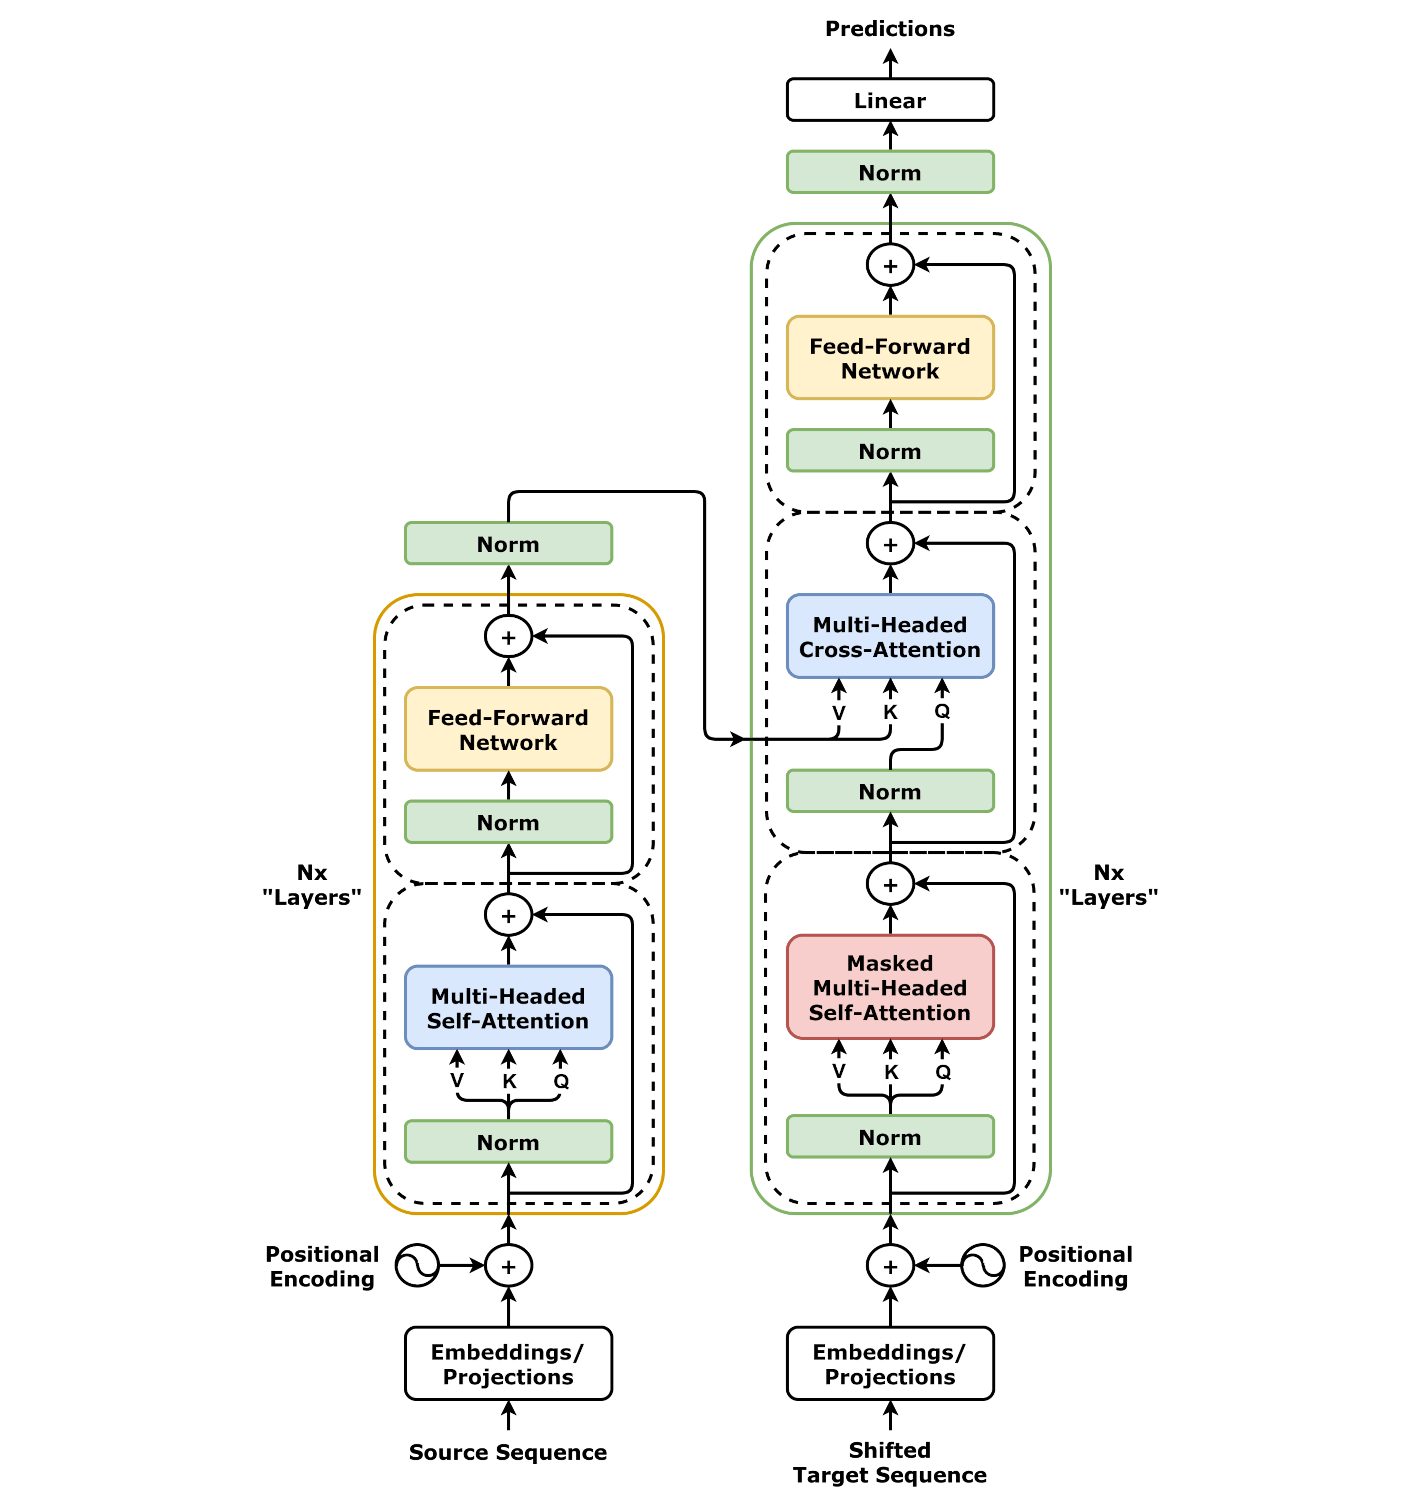
\includegraphics[width=1.05\linewidth]{Images/cap1/Transformer,_full_architecture.png}
	\caption{Transformer: a sinistra l'encoder, a destra il decoder \cite{transformervisuals}.}
	\label{fig:transformer}
\end{figure}

Nonostante esistano diverse varianti del Transformer, tutte condividono le seguenti componenti principali e sequenza di operazioni \cite{phuong2022formalalgorithmstransformers}:
\begin{itemize}
	\item \textbf{Tokenizer}: Converte il testo in input in una sequenza di token, che rappresentano le unità di base elaborate dal modello.
	\item \textbf{Embedding Layer}: Mappa i token in vettori di embedding, i quali catturano le relazioni semantiche tra le parole, includendo informazioni sia sul significato che sulla posizione dei token nella sequenza.
	\item \textbf{Transformer Layer}: Costituiscono il cuore del modello. Ogni Transformer layer estrae informazioni sempre più complesse attraverso più livelli. Questi strati multilivello comprendono sia l'encoder che il decoder (nella versione standard del Transformer).
	\item \textbf{Un-embedding Layer}: Converte le rappresentazioni vettoriali finali in una distribuzione di probabilità sui token del vocabolario, permettendo così di generare il testo in output.
\end{itemize}
Le componenti verranno ora esaminate nel dettaglio:

\subsubsection{Tokenizer}
Il Transformer non può processare nativamente dati di tipo testuale, si occupa invece di analizzare sequenze numeriche. Per questo motivo è necessario convertire il testo in input in qualche modo, il primo passo consiste nell'associare un intero per ogni carattere o comunque per una piccola sequenza di caratteri (token). Il set di tutti i token generati viene chiamato vocabolario.

\subsubsection{Embedding Layer}
Ogni token viene convertito in un vettore di embedding \cite{mikolov2013distributedrepresentationswordsphrases}, e la corrispondenza tra il token e il suo vettore viene salvata in una \textit{"lookup table"}. La dimensione di questi vettori di embedding, nota anche come hidden dimension \cite{gpt2backbone} o embedding size \cite{devlin2019bertpretrainingdeepbidirectional}, varia in base all'implementazione utilizzata. Nel paper originale viene indicata con $d_{\text{model}} = 512$ \cite{vaswani2023attentionneed}, ma esistono modelli con dimensioni differenti, come ad esempio GPT-2 con $d_{\text{model}} = 768$ \cite{gpt2backbone}, BERT con $d_{\text{model}} = 768$ \cite{devlin2019bertpretrainingdeepbidirectional}, o T5 con $d_{\text{model}} = 1024$ \cite{raffel2023exploringlimitstransferlearning}.

Grazie a questa conversione, il Transformer è in grado di interpretare il testo in modo più strutturato, ma emergono alcune limitazioni. In particolare, parole diverse con significato simile (sinonimia) possono produrre embedding differenti, mentre parole con più significati (polisemia) tendono a generare lo stesso embedding indipendentemente dal contesto. Questo porta spesso a rappresentazioni ambigue e potenzialmente errate.
Per ovviare a queste limitazioni, si possono usare modelli di embedding pre-addestrati come Word2Vec \cite{mikolov2013efficientestimationwordrepresentations}, sviluppato da un team di Google guidato da Tomas Mikolov nel 2013, o GloVe \cite{pennington-etal-2014-glove}, sviluppato dalla Stanford University. Entrambi gli approcci catturano relazioni semantiche tra le parole grazie a tecniche basate su co-occorrenza e distribuzione dei termini.
In alternativa, è possibile addestrare un modello di embedding specifico per il task, per ottenere rappresentazioni più precise nel contesto d'uso. Una delle soluzioni avanzate a questo problema è l'uso di modelli che supportano i multi-sense embeddings \cite{camachocollados2018wordsenseembeddingssurvey,reisinger-mooney-2010-multi}, i quali assegnano rappresentazioni vettoriali diverse a parole con significati differenti a seconda del contesto in cui appaiono, migliorando così la gestione di sinonimia e polisemia.

\subsubsection{Transformer Layer}
\textit{Vedi Paragrafo} \ref{sec:transformer-layer} \textit{per una trattazione completa.}

\subsubsection{Un-embedding Layer}
A seguito dell'elaborazione dell'input, il vettore di output viene convertito in una distribuzione di probabilità sui token del vocabolario. Questo processo è noto come \textit{"un-embedding"} e viene realizzato attraverso un layer di output softmax, che restituisce la probabilità di ciascun token in base al contesto.
\begin{align}
	\text{UnEmbed}(x) = \text{softmax}(xW + b)
\end{align}
Il token con la probabilità più alta viene selezionato come output finale.

\subsection{Transformer Layer}
\label{sec:transformer-layer}
I modelli Transformer sono costituiti da più strati di Transformer Layer, ognuno dei quali può assumere configurazioni differenti a seconda dell'implementazione e dell'utilizzo specifico che verrà fatto. In particolare, si farà riferimento alla versione originale proposta da Vaswani et al. \cite{vaswani2023attentionneed}, che comprende sia un encoder che un decoder.
\begin{figure}[!t]
	\centering
	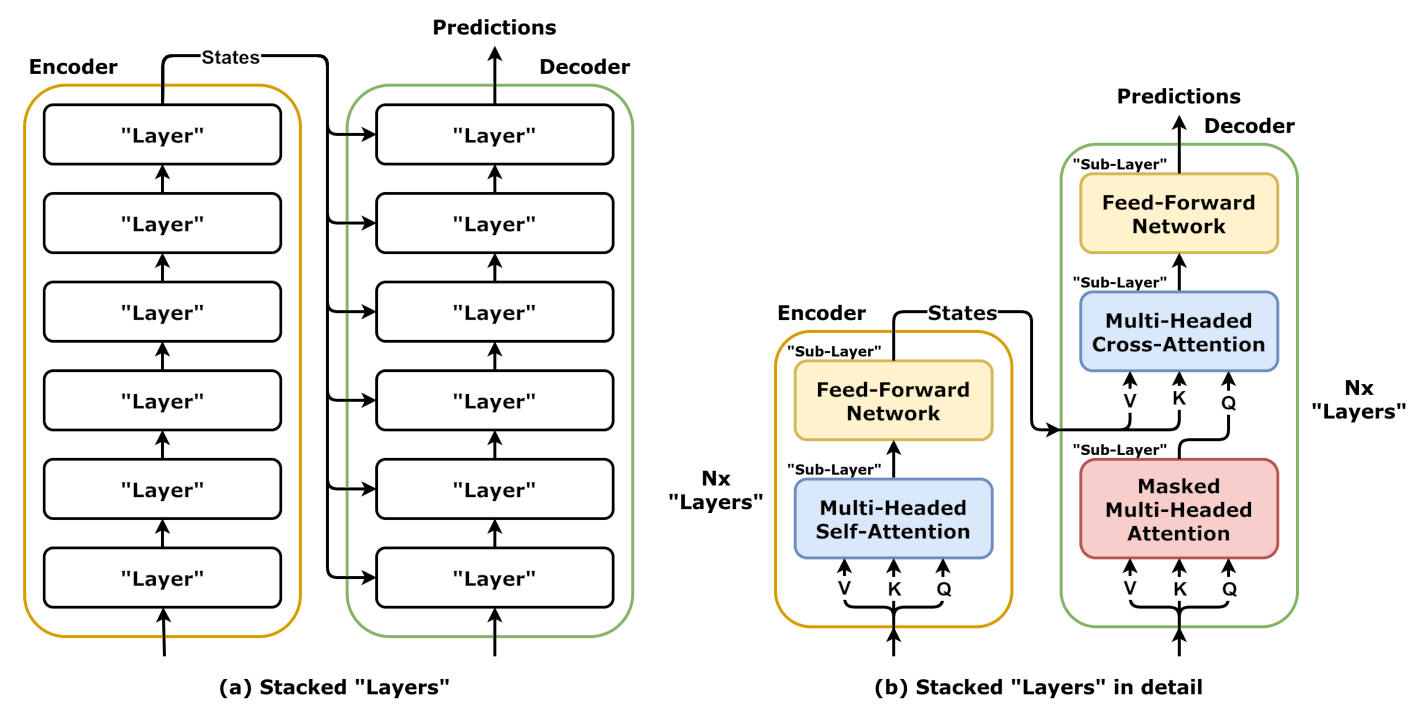
\includegraphics[width=\linewidth]{Images/cap1/Transformer,_stacked_layers_and_sublayers.png}
	\caption{Architettura a strati del Transformer.}
	\label{fig:transformer-sublayers}
\end{figure}
Il numero di layer, la dimensione dei vettori di embedding e la dimensione dei feed-forward neural network sono iperparametri che possono essere regolati per adattare la rete neurale a diversi compiti e dataset.
In generale, un numero maggiore di layer permette al Transformer di catturare relazioni più complesse e di apprendere rappresentazioni più dettagliate, ma richiede anche più risorse computazionali e tempo di addestramento.
A seguire le caratteristiche implementative del Transformer Layer presentato nel paper originale.

\subsubsection{Encoder}
L'encoder è costituito da una pila di \(N\) layer identici (6 nell'originale di Vaswani et al.) \cite{vaswani2023attentionneed}, ciascuno dei quali opera in parallelo sugli input. Ogni layer è composto da due sub-layer principali:
\begin{itemize}
	\item \textbf{Multi-Headed Self-Attention}: Questo meccanismo consente ad esso di catturare le relazioni tra le parole all'interno della stessa sequenza. Ogni parola può "attenzionare" tutte le altre parole della sequenza, calcolando un peso relativo in base alla loro rilevanza nel contesto. Grazie a diverse "teste" di attenzione, il modello può osservare la sequenza da prospettive diverse, cogliendo dipendenze sia a breve che a lungo termine. Questo è fondamentale per comprendere le relazioni semantiche complesse all'interno di una frase e per gestire le dipendenze a lungo raggio.
	\item \textbf{Feed-Forward Neural Network}: Dopo la fase di attenzione, ogni vettore di embedding viene elaborato da uno o più layer feed-forward. Questa rete opera in parallelo su tutti i token della sequenza, applicando una trasformazione non lineare che permette al modello di arricchire le rappresentazioni dei token e di catturare pattern più complessi. La rete feed-forward è costituita da due layer densi con una funzione di attivazione intermedia, generalmente una ReLU (Rectified Linear Unit), per introdurre non linearità nell'elaborazione. In certi casi, si possono utilizzare funzioni di attivazione diverse, come la GELU (Gaussian Error Linear Unit), che ha dimostrato di migliorare le prestazioni in alcuni compiti \cite{hendrycks2023gaussianerrorlinearunits}.
\end{itemize}
Entrambi i sub-layer sono seguiti da una Residual Connection e da un Layer Normalization \cite{ba2016layernormalization}. Le Residual Connections permettono di "saltare" i sub-layer e aggiungono l'input originale direttamente all'output del sub-layer stesso, facilitando il flusso del gradiente attraverso i layer. Questo accorgimento aiuta a prevenire il problema del vanishing gradient, che ostacolerebbe l'apprendimento nei modelli profondi. Inoltre, esse ne accelerano il processo, poiché mantengono in circolazione informazioni non modificate, mentre la rete si concentra sulla modellazione di pattern più complessi.
Il Layer Normalization, applicato dopo ogni Residual Connection, stabilizza l'addestramento mantenendo il range delle attivazioni all'interno di una scala gestibile. Questo aiuta il modello a convergere più rapidamente durante il processo di ottimizzazione, riducendo l'instabilità causata dalle variazioni nei valori delle attivazioni. Esistono diverse alternative al Layer Normalization come il Root Mean Square Layer Normalization (RMS-LN) \cite{zhang2019rootmeansquarelayer}, il BatchNorm usato nei modelli della famiglia Llama, o altri \cite{https://doi.org/10.5281/zenodo.3525484}.

\paragraph{Noam Learning Rate Scheduler}
Un'altra strategia utilizzata per stabilizzare l'addestramento è l'impiego di un meccanismo di warmup del learning rate, implementato tramite il cosiddetto Noam Learning Rate Scheduler \cite{noamlearningrate,vaswani2023attentionneed}. Questo scheduler aumenta gradualmente il learning rate nei primi \(w\) step dell'addestramento (warmup steps), per poi ridurlo in proporzione inversa alla radice quadrata del numero \(t\) di passi temporali.
\begin{align}
	\text{learning rate} = \alpha \frac{1}{\sqrt{d_{\text{model}}}} \min \left(\frac{1}{\sqrt{t}}, \frac{t}{w^{3/2}} \right)
	\label{eq:noam-scheduler}
\end{align}
Tale schema evita oscillazioni improvvise nel processo di ottimizzazione e garantisce una fase iniziale di esplorazione dello spazio delle soluzioni, migliorando la stabilità complessiva della rete.

Tuttavia, ricerche successive hanno dimostrato che il meccanismo di warmup non è sempre strettamente necessario, poiché, applicando la normalizzazione prima della multi-head attention, piuttosto che dopo, si può ridurre o eliminare la necessità del warmup, stabilizzando comunque l'apprendimento e velocizzando la convergenza \cite{xiong2020layernormalizationtransformerarchitecture} (vedi \figurename{~\ref{fig:encoder}}).
\begin{figure}[!t]
    \centering
    \begin{minipage}{0.48\textwidth}
        \centering
		\hspace*{-2cm}
        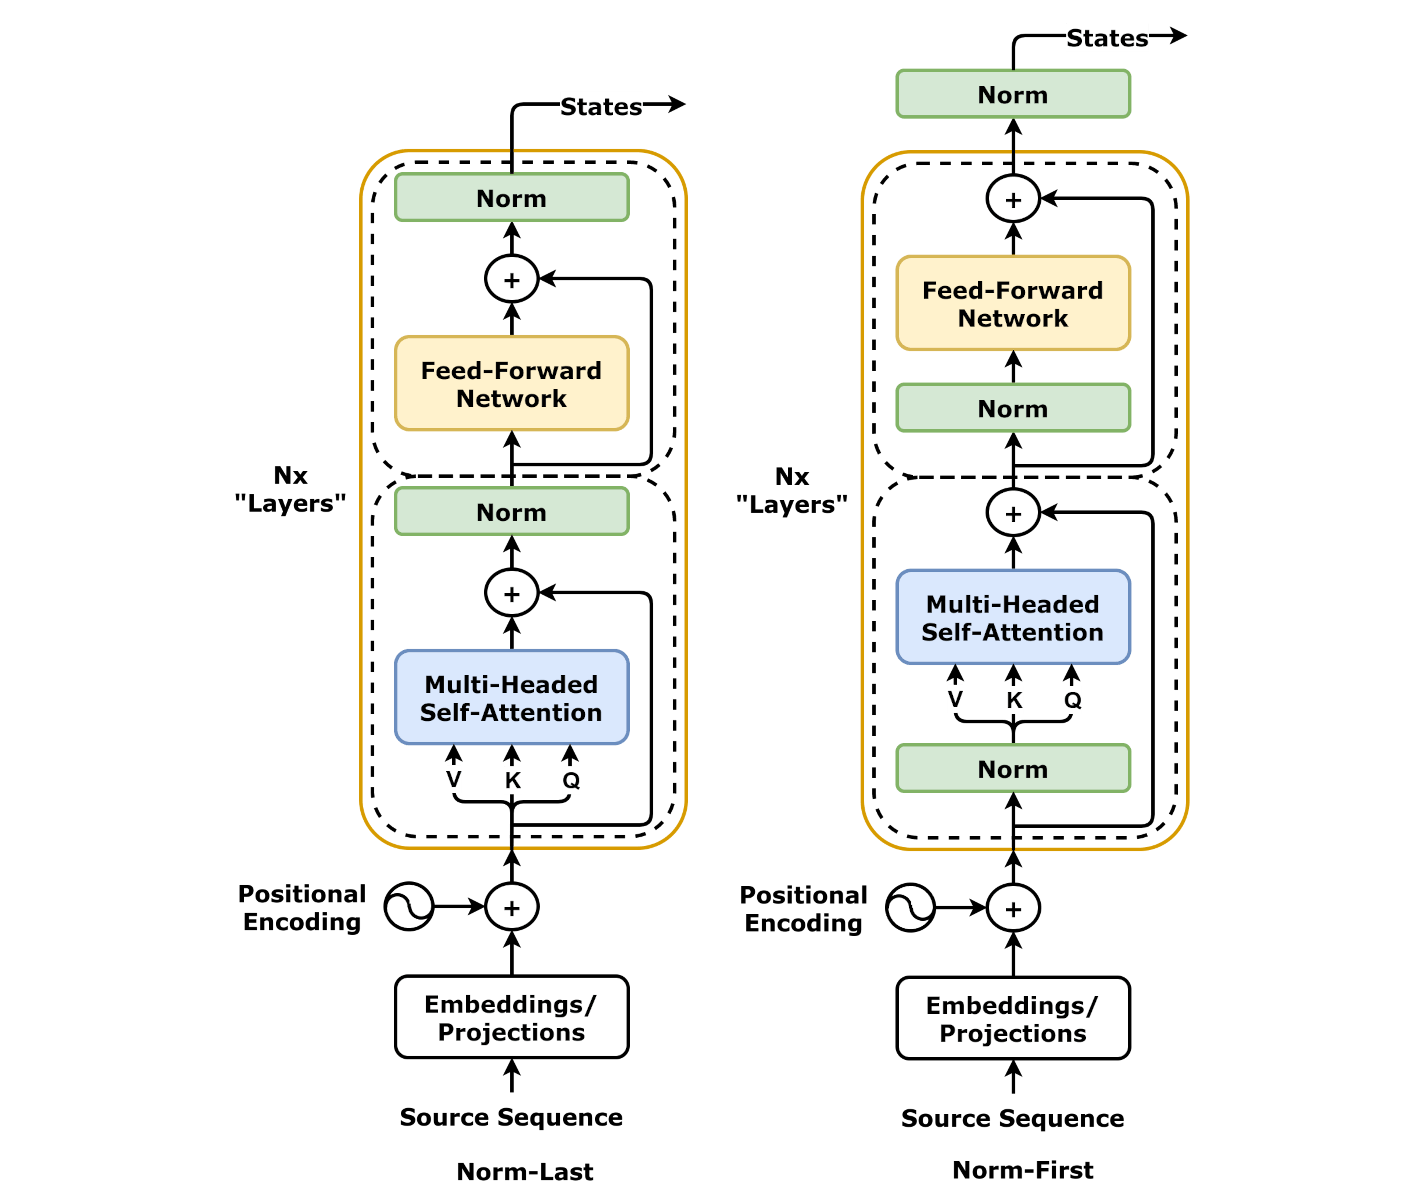
\includegraphics[width=1.5\linewidth]{Images/cap1/Transformer_encoder,_with_norm-first_and_norm-last.png}
        \caption{Differenza tra Encoder Norm Last ed Encoder Norm First}
        \label{fig:encoder}
    \end{minipage}
    \hfill
    \begin{minipage}{0.48\textwidth}
        \centering
		\hspace*{-0.7cm}
        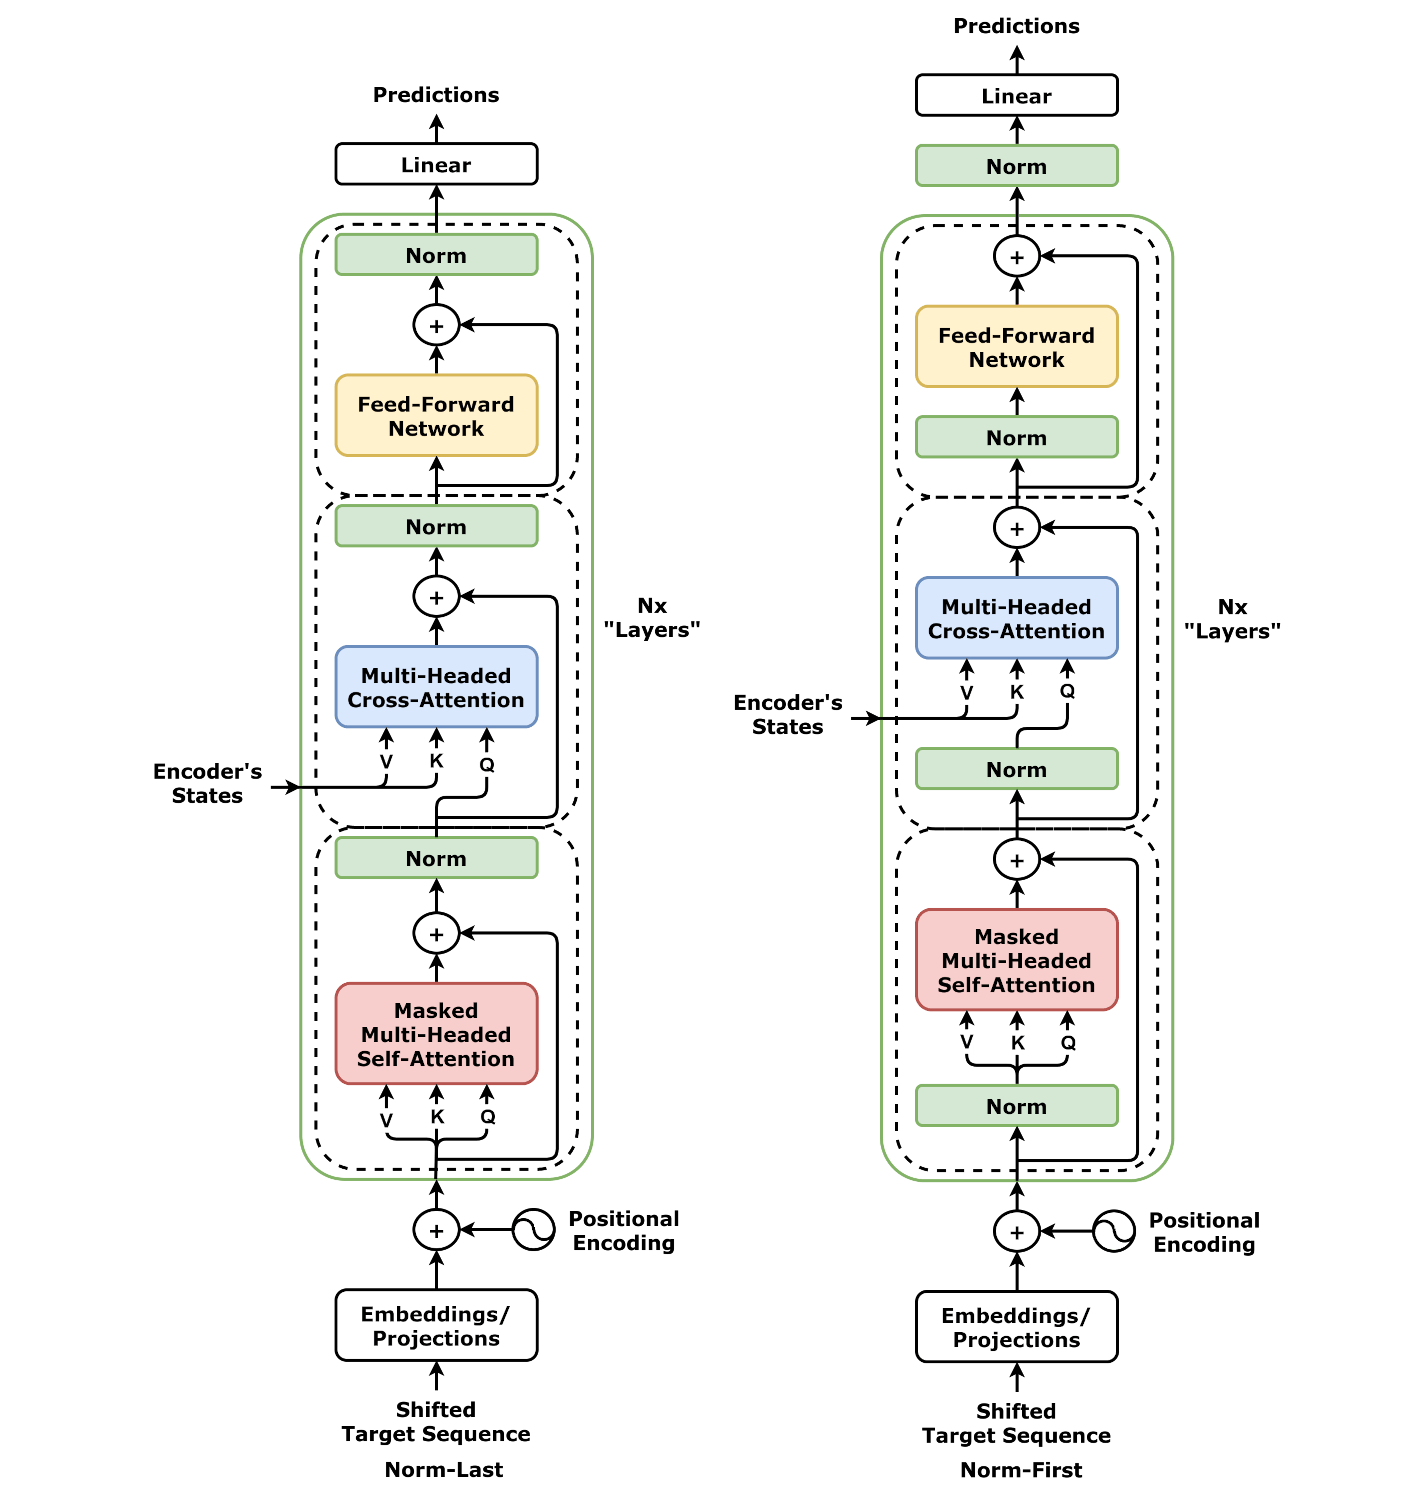
\includegraphics[width=1.2\linewidth]{Images/cap1/Transformer_decoder,_with_norm-first_and_norm-last.png}
        \caption{Differenza tra Decoder Norm Last e Decoder Norm First}
        \label{fig:decoder}
    \end{minipage}
\end{figure}

\subsubsection{Decoder}
Il decoder del Transformer, come l'encoder, è costituito da una pila di \(N\) layer identici (6 in quello originale). Ogni layer del decoder condivide alcune somiglianze con i layer dell'encoder, ma include anche un'importante differenza, data dalla presenza di un terzo sub-layer. Oltre ai due sub-layer che già troviamo nell'encoder, ovvero il Multi-Head Self-Attention Mechanism e la Feed-Forward Neural Network, il decoder introduce un ulteriore sub-layer, chiamato Cross-Attention, che serve a integrare le informazioni elaborate dall'encoder.
I layer del decoder possono essere descritti come segue:
\begin{itemize}
	\item \textbf{Masked Multi-Headed Self-Attention}: Questo sub-layer è simile a quello utilizzato nell'encoder, ma con una differenza fondamentale. Nel decoder, viene applicata una maschera causale (vedi Paragrafo \ref{sec:masked-multi-head-attention}) che impedisce al modello di "guardare" i token futuri. In altre parole, il decoder può prestare attenzione solo ai token già generati e non a quelli successivi, il che è cruciale nei compiti di generazione sequenziale come la traduzione automatica. La maschera causale serve a mantenere la coerenza temporale durante la generazione, garantendo che il modello generi il testo in modo incrementale, senza conoscere in anticipo i token futuri.
	\item \textbf{Multi-Headed Cross-Attention}: Questo secondo sub-layer applica la Multi-Head Attention non solo sui token interni alla sequenza di input del decoder, ma anche sulle rappresentazioni intermedie prodotte dall'encoder. In questo modo, il decoder è in grado di combinare le informazioni che ha già elaborato con le rappresentazioni dell'input elaborate dall'encoder. Questa fase permette al decoder di integrare e "attenzionare" specifiche parti dell'input in base a ciò che ha già generato, creando una connessione tra l'input e l'output che il modello sta costruendo.
	\item \textbf{Feed-Forward Neural Network}: Come nell'encoder, anche qui ogni token è elaborato indipendentemente da una rete neurale feed-forward, che arricchisce le rappresentazioni attraverso trasformazioni non lineari. Questa rete è condivisa in ogni layer e applicata in parallelo su tutti i token della sequenza di output.
\end{itemize}
Tutti e tre i sub-layer sono seguiti da Residual Connections e da un Layer Normalization. Anche in questo caso vale l'osservazione precedente relativa all'ordine di applicazione della normalizzazione nella sequenza di operazioni \cite{xiong2020layernormalizationtransformerarchitecture} (vedi \figurename{~\ref{fig:decoder}}).

\paragraph{Norm-Last vs Norm-First Formula}
L'output generato da ogni sub-layer del Transformer può essere descritto come segue:

Nella versione Norm-Last:
\begin{align}
	\text{Output} = \text{LayerNorm}(x + \text{Sublayer}(x))
\end{align}
Dove \(x\) rappresenta l'input del sub-layer e \(\text{Sublayer}(x)\) la sua elaborazione. La Residual Connection aggiunge l'input originale all'output del sub-layer, mentre il Layer Normalization stabilizza l'addestramento normalizzando le attivazioni.

Oppure nella versione Norm-First:
\begin{align}
	\text{Output} = x + \text{Sublayer}(\text{LayerNorm}(x))
\end{align}

\section{Attention Is All We Need}
Il meccanismo di attenzione è alla base del Transformer ed è fondamentale per gestire le dipendenze tra parole in una sequenza. Può essere descritto come un'operazione di mappatura che prende in input una query e la confronta con un insieme di chiavi (keys) e valori (values), tutti rappresentati da vettori. La query viene confrontata con ogni chiave per calcolare un punteggio di somiglianza, che determina quanto una chiave è rilevante per la query.
Più formalmente, si può dire che l'obiettivo sia calcolare un'uscita pesata dei valori in base alla somiglianza tra la query e le chiavi. Ogni valore viene poi moltiplicato per il punteggio corrispondente, e l'output finale è una somma pesata dei valori.
\begin{itemize}
	\item \textbf{Query}: La query rappresenta l'elemento di input per il quale vogliamo ottenere informazioni rilevanti, in base alle chiavi e ai valori.
	\item \textbf{Keys}: Le chiavi rappresentano gli elementi con cui la query viene confrontata. Ogni chiave ha un valore associato.
	\item \textbf{Values}: I valori sono le informazioni associate a ciascuna chiave, che verranno utilizzate per calcolare l'output.
\end{itemize}
L'output è una somma pesata dei valori, dove i pesi sono dati dalla compatibilità (somiglianza) tra la query e le chiavi, calcolata tipicamente tramite un'operazione come il dot-product (prodotto scalare).
Se necessario (come nel caso del Transformer originale), il prodotto scalare può essere scalato per evitare divergenze nei valori dei pesi causati dall'applicazione della funzione softmax su valori elevati.
\begin{figure}[!t]
	\centering
	\begin{minipage}{0.48\textwidth}
		\centering
		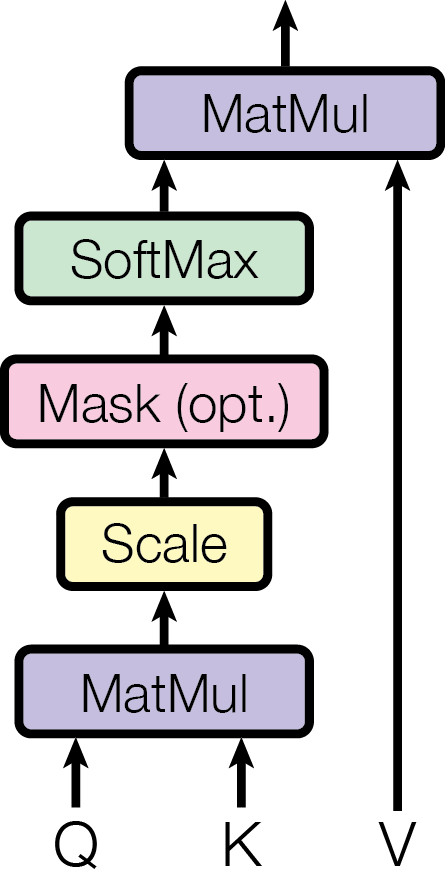
\includegraphics[width=0.5\linewidth]{Images/cap1/ModalNet-19.png}
		\caption{Scaled Dot-Product}
		\label{fig:scaleddotproduct}
	\end{minipage}
	\hfill
	\begin{minipage}{0.48\textwidth}
		\centering
		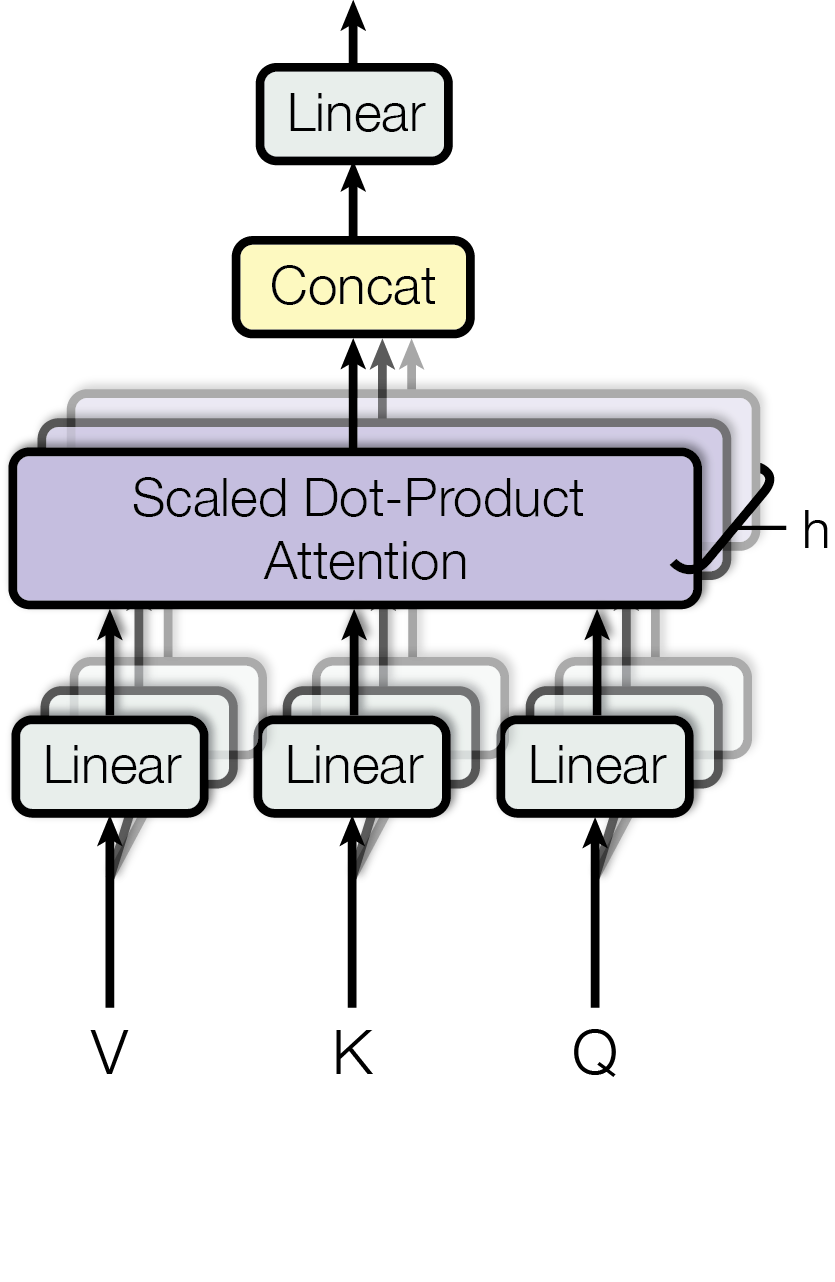
\includegraphics[width=0.65\linewidth]{Images/cap1/ModalNet-20.png}
		\caption{Multi-Head Attention}
		\label{fig:multihead}
	\end{minipage}
\end{figure}
Esistono diverse varianti del meccanismo di attenzione che nel tempo si sono evolute per permettere al modello di diventare più efficiente e, dunque, di avere prestazioni più elevate, come nel caso del Reformer \cite{kitaev2020reformerefficienttransformer} o tramite l'implementazione Flash Attention \cite{dao2022flashattentionfastmemoryefficientexact} che è ottimizzata per calcoli su GPU e TPU in quanto esegue moltiplicazioni tra blocchi di matrici in parallelo. Esiste anche la variante ALiBi (Attention with Linear Biases) \cite{press2022trainshorttestlong} che implementa un meccanismo di positional encoding (vedi Paragrafo \ref{sec:positional-encoding}) aggiuntivo direttamente all'interno del meccanismo di attenzione.

\subsection{Scaled Dot-Product Attention}
Nel paper originale il meccanismo di attenzione viene definito Scaled Dot-Product Attention (vedi \figurename{~\ref{fig:scaleddotproduct}}). L'input dello stesso consiste in un set di vettori query e chiavi di dimensioni \(d_k\), e un set di valori di dimensioni \(d_v\). Vengono calcolati i prodotti scalari di una query con tutte le chiavi e si divide ciascuno di essi per \(\sqrt{d_k}\) (scaling). Infine, si applica una funzione softmax per ottenere i pesi di attenzione sui valori.
Questa procedura viene effettuata su più vettori query parallelamente. Tutti i vettori query vengono inglobati in una matrice \(Q\), i vettori chiave in una matrice \(K\) e i vettori valori in una matrice \(V\). L'output dell'operazione di attenzione è una matrice calcolata con la seguente formula:
\begin{align}
	\text{Attention}(Q, K, V) = \text{softmax}\left(\frac{QK^T}{\sqrt{d_k}}\right)V
\end{align}

\subsection{Multi-Head Attention}
Per catturare relazioni complesse e multidimensionali tra le parole, il Transformer utilizza il meccanismo di Multi-Head Attention (vedi \figurename{~\ref{fig:multihead}}). Questo approccio consente ad esso di apprendere diverse rappresentazioni delle parole attraverso diverse "teste" di attenzione, ciascuna delle quali si concentra su aspetti diversi della sequenza. Ogni testa di attenzione calcola i pesi in modo indipendente, permettendo al modello di cogliere relazioni intricate tra i token e di apprendere rappresentazioni più ricche e dettagliate.

Anziché eseguire una singola operazione di attenzione utilizzando chiavi, valori e query di dimensione \(d_{model}\) (la dimensione dei vettori di embedding), il meccanismo Multi-Head Attention prevede che queste grandezze siano proiettate linearmente \(h\) volte con diverse proiezioni apprese per ottenere chiavi, valori e query di dimensione \(d_k\) e \(d_v\). Su ognuna di queste versioni proiettate di chiavi, valori e query, l'operazione di attenzione viene eseguita in parallelo, producendo come risultato valori in uscita di dimensione \(d_v\).

I risultati delle diverse teste vengono quindi concatenati e proiettati nuovamente per ottenere l'output finale, come mostrato in \figurename{~\ref{fig:multihead}}. Questo processo consente al modello di osservare diversi sottospazi di rappresentazione contemporaneamente, migliorando così la capacità di catturare informazioni da più posizioni nella sequenza \cite{bertattention}. Con un'unica testa di attenzione, infatti, l'operazione media queste informazioni, riducendo la capacità del modello di apprendere relazioni multidimensionali.

Matematicamente, il meccanismo Multi-Head Attention può essere descritto come:
\begin{align}
	\text{MultiHeadedAttention}(Q, K, V) = \text{Concat}(\text{head}_1, \ldots, \text{head}_h)W^O
\end{align}
Dove:
\vspace{-0.25cm}
\begin{align}
	\text{head}_i = \text{Attention}(QW_i^Q, KW_i^K, VW_i^V)
\end{align}
Le proiezioni sono realizzate tramite le matrici dei parametri:
\begin{align}
	W_i^Q \in \mathbb{R}^{d_{model} \times d_k}, \quad W_i^K \in \mathbb{R}^{d_{model} \times d_k}, \quad W_i^V \in \mathbb{R}^{d_{model} \times d_v}, \quad W^O \in \mathbb{R}^{hd_v \times d_{model}}
\end{align}
Nel prototipo originale, sono state utilizzate \(h = 8\) teste di attenzione in parallelo, con \(d_k = d_v = d_{model}/h = 64\). Grazie alla riduzione della dimensione di ciascuna testa, il costo computazionale complessivo rimane simile a quello dell'attenzione a singola testa con la dimensionalità completa.
Il sistema di attenzione multi-testa viene utilizzato in maniera diversa a seconda che si tratti di quello dell'encoder, del decoder o del cross-attention.

\subsubsection{Multi-Headed Self-Attention (Encoder)}
Nell'auto-attenzione nell'encoder, le query, le chiavi e i valori provengono tutti dalla stessa sorgente, ovvero l'output del livello precedente dell'encoder. Ogni posizione nell'encoder può prestare attenzione a tutte le altre posizioni della sequenza elaborata fino a quel punto. Questo consente al modello di catturare relazioni globali tra le parole e costruire rappresentazioni più ricche del contesto testuale. Questo tipo di auto-attenzione è cruciale per comprendere la struttura sintattica e semantica del testo.

\subsubsection{Multi-Headed Cross-Attention (Encoder-Decoder)}
Nell'attività di attenzione encoder-decoder, le query provengono dal livello precedente del decoder, mentre le chiavi e i valori sono generati dall'output dell'encoder. Questo permette a ogni posizione nel decoder di "attenzionare" tutte le posizioni della sequenza di input. In pratica, l'attenzione encoder-decoder consente al decoder di focalizzarsi su specifiche parti della sequenza di input per generare l'output corretto. Questo meccanismo è tipico nei modelli di sequence-to-sequence \cite{sutskever2014sequencesequencelearningneural}, come nei tradizionali modelli di traduzione automatica.

\subsubsection{Masked Multi-Headed Self-Attention (Decoder)}
\label{sec:masked-multi-head-attention}
Anche nel decoder troviamo livelli di auto-attenzione, ma con una particolarità importante: ogni posizione nel decoder può prestare attenzione solo alle posizioni precedenti o uguali della sequenza già generata. Questo comportamento è essenziale per preservare la proprietà auto-regressiva del modello, ovvero l'abilità del decoder di generare il testo in modo sequenziale, senza poter "guardare" il futuro. Per implementare questa restrizione, si applica una maschera che blocca il flusso di informazioni verso destra, mascherando con \(-\infty\)  le connessioni non valide nel calcolo della softmax.

La maschera viene indicata con \(M\) e la funzione di attenzione viene modificata come segue:
\begin{align}
	\text{MaskedAttention}(Q, K, V) = \text{softmax}\left(\frac{QK^T}{\sqrt{d_k}} + M\right)V
\end{align}
Una maschera tipica per il decoder è una matrice triangolare strettamente superiore, che blocca le connessioni tra le posizioni future. Questo garantisce che il modello generi il testo in modo incrementale, senza conoscere in anticipo i token successivi. Questa maschera è chiamata "Maschera Causale" (Causal Mask) e viene applicata a ciascuna testa di attenzione nel decoder.
\begin{align}
	M_{ij} = \begin{cases}
		0 & \text{se } i \leq j \\
		-\infty & \text{altrimenti}
	\end{cases}
\end{align}

\subsection{Position-wise Feed-Forward Networks}
Oltre ai layer attenzionali, sia encoder che decoder sono dotati di un layer di feed-forward neural network, che opera in modo indipendente su ciascuna posizione della sequenza. Questo layer è composto da due layer densi (fully connected) con una funzione di attivazione intermedia, generalmente una ReLU.
\begin{align}
	\text{FFN}(x) = \text{ReLU}(xW_1 + b_1)W_2 + b_2
\end{align}
Solitamente la dimensione dei vettori di embedding viene aumentata nel primo layer e poi ridotta nel secondo, per permettere alla rete di apprendere rappresentazioni più complesse e di ridurre la dimensionalità prima di passare al livello successivo. Questo layer è seguito da un'altra Residual Connection e da un Layer Normalization, per facilitare il flusso del gradiente e stabilizzare l'addestramento.
Sebbene le trasformazioni lineari siano identiche per ogni posizione della sequenza, i parametri utilizzati variano da un livello all'altro. Questo processo può essere descritto come due convoluzioni con kernel di dimensione 1.

\subsection{Positional Encoding}
\label{sec:positional-encoding}
Infine (anche se viene trattato all'inizio della sequenza come parte dell'input, vedi \figurename{~\ref{fig:transformer}}), il Transformer utilizza un meccanismo di codifica posizionale per introdurre informazioni sulla posizione delle parole nella sequenza. Poiché la rete neurale non contiene unità ricorrenti o convoluzionali, che di solito catturano la posizione temporale delle parole, è necessario fornire al modello un modo per distinguere le parole in base alla loro posizione.

Dunque, per risolvere questo problema è possibile aggiungere vettori di posizione (positional encodings) ai vettori di embedding in input. Questi vettori hanno la stessa dimensione dei vettori di embeddings  \(d_{\text{model}}\) così da poter essere sommati direttamente. Per calcolare i vettori di posizione, si utilizzano funzioni trigonometriche \cite{dufter2021positioninformationtransformersoverview}, che permettono di codificare informazioni sulla posizione in modo non lineare. Nel paper originale, vengono utilizzate le seguenti funzioni:
\begin{align}
	\text{PE}_{(pos, 2i)} = \sin\left(\frac{pos}{10000^{2i/d_{\text{model}}}}\right), \quad \text{PE}_{(pos, 2i+1)} = \cos\left(\frac{pos}{10000^{2i/d_{\text{model}}}}\right)
\end{align}
Dove \(pos\) rappresenta la posizione della parola nella sequenza e \(i\) la dimensione del vettore di embedding. In questo modo ogni dimensione del vettore di posizione corrisponde ad una sinusoide e le lunghezze d'onda variano in base alla posizione formando una progressione geometrica che va da \(2\pi\) a \(10000 \cdot 2\pi\). Questa funzione è stata scelta poiché si ipotizzava che avrebbe facilitato il modello nell'apprendimento delle posizioni relative poiché per ogni offset costante \(k\), \(\text{PE}_{(pos + k)}\) può essere rappresentato come una funzione lineare di \(\text{PE}_{(pos)}\).

Esistono varianti che utilizzano approcci convoluzionali \cite{gehring2017convolutionalsequencesequencelearning} che hanno dato risultati simili, ma si preferisce usare funzioni sinusoidali perché si ritiene che consentano al modello di generalizzare meglio su sequenze di lunghezza superiore rispetto a quelle incontrate durante l'addestramento. Successivamente si è scoperto che anche senza applicare la codifica posizionale, si è in grado di apprendere informazioni posizionali grazie all'applicazione della maschera causale nel decoder \cite{haviv2022transformerlanguagemodelspositional}.
Successivamente sono stati sviluppati algoritmi di Relative Positional Encoding \cite{shaw2018selfattentionrelativepositionrepresentations} che permettono la codifica delle posizioni relative tra le parole, migliorando la capacità del Transformer di catturare relazioni spaziali tra le parole. Questo approccio è differente da quello originale, che codifica solo la posizione assoluta delle parole \cite{ke2021rethinkingpositionalencodinglanguage}.

\chapter{Retrieval-Augmented Generation}
I Large Language Models sono uno strumento estremamente potente e versatile. Tuttavia, possiedono anche numerose limitazioni e difetti che possono renderli inaffidabili in alcune situazioni o inadatti per determinati compiti. Inoltre, la loro conoscenza è limitata a quanto appreso durante la fase di addestramento, e le loro funzionalità si concentrano principalmente sulla generazione di testo. Per superare queste limitazioni sono stati sviluppati diversi accorgimenti che spaziano dal semplice Prompt Engineering al Fine Tuning, fino alla progettazione di architetture più complesse in grado di integrare capacità di ragionamento all'interno del modello.
Nello sviluppo del progetto presentato in questa tesi, sono state impiegate molte di queste tecniche (vedi Capitolo \ref{cap:omnibot1}), con un focus particolare su un approccio basato su un'architettura denominata Retrieval-Augmented Generation.

\section{Cos'è RAG?}
Retrieval-Augmented Generation (RAG) \cite{whatisrag,raghandbook,gao2024retrievalaugmentedgenerationlargelanguage} è un'architettura che combina tecniche di Information Retrieval (IR) con tecniche di Natural Language Generation (NLG) per generare risposte più accurate e coerenti. L'idea alla base di RAG è quella di integrare un modulo di retrieval all'interno di un LLM per fornire ad esso informazioni aggiuntive e contestuali durante la fase di generazione del testo. In questo modo, il modello può accedere a una vasta quantità di conoscenza esterna e utilizzarla per migliorare la qualità delle risposte generate.

Il funzionamento della versione elementare di RAG è abbastanza semplice e consiste in due fasi principali:
\begin{enumerate}
    \item \textbf{Retrieval}: In questa fase, l'LLM utilizza un modulo di retrieval (retriever) per recuperare i documenti rilevanti da una base di conoscenza esterna (knowledge base). Il retriever può essere progettato in diversi modi, ma in generale, il suo compito principale è quello di identificare i documenti che contengono le informazioni necessarie per rispondere alla domanda posta.
    \item \textbf{Generation}: Una volta recuperati i documenti rilevanti, il modello utilizza le informazioni contenute in essi per generare una risposta accurata e coerente. Il generatore può essere un qualsiasi LLM pre-addestrato.
\end{enumerate}

\section{Come funziona RAG?}
\begin{figure}[!t]
    \centering
    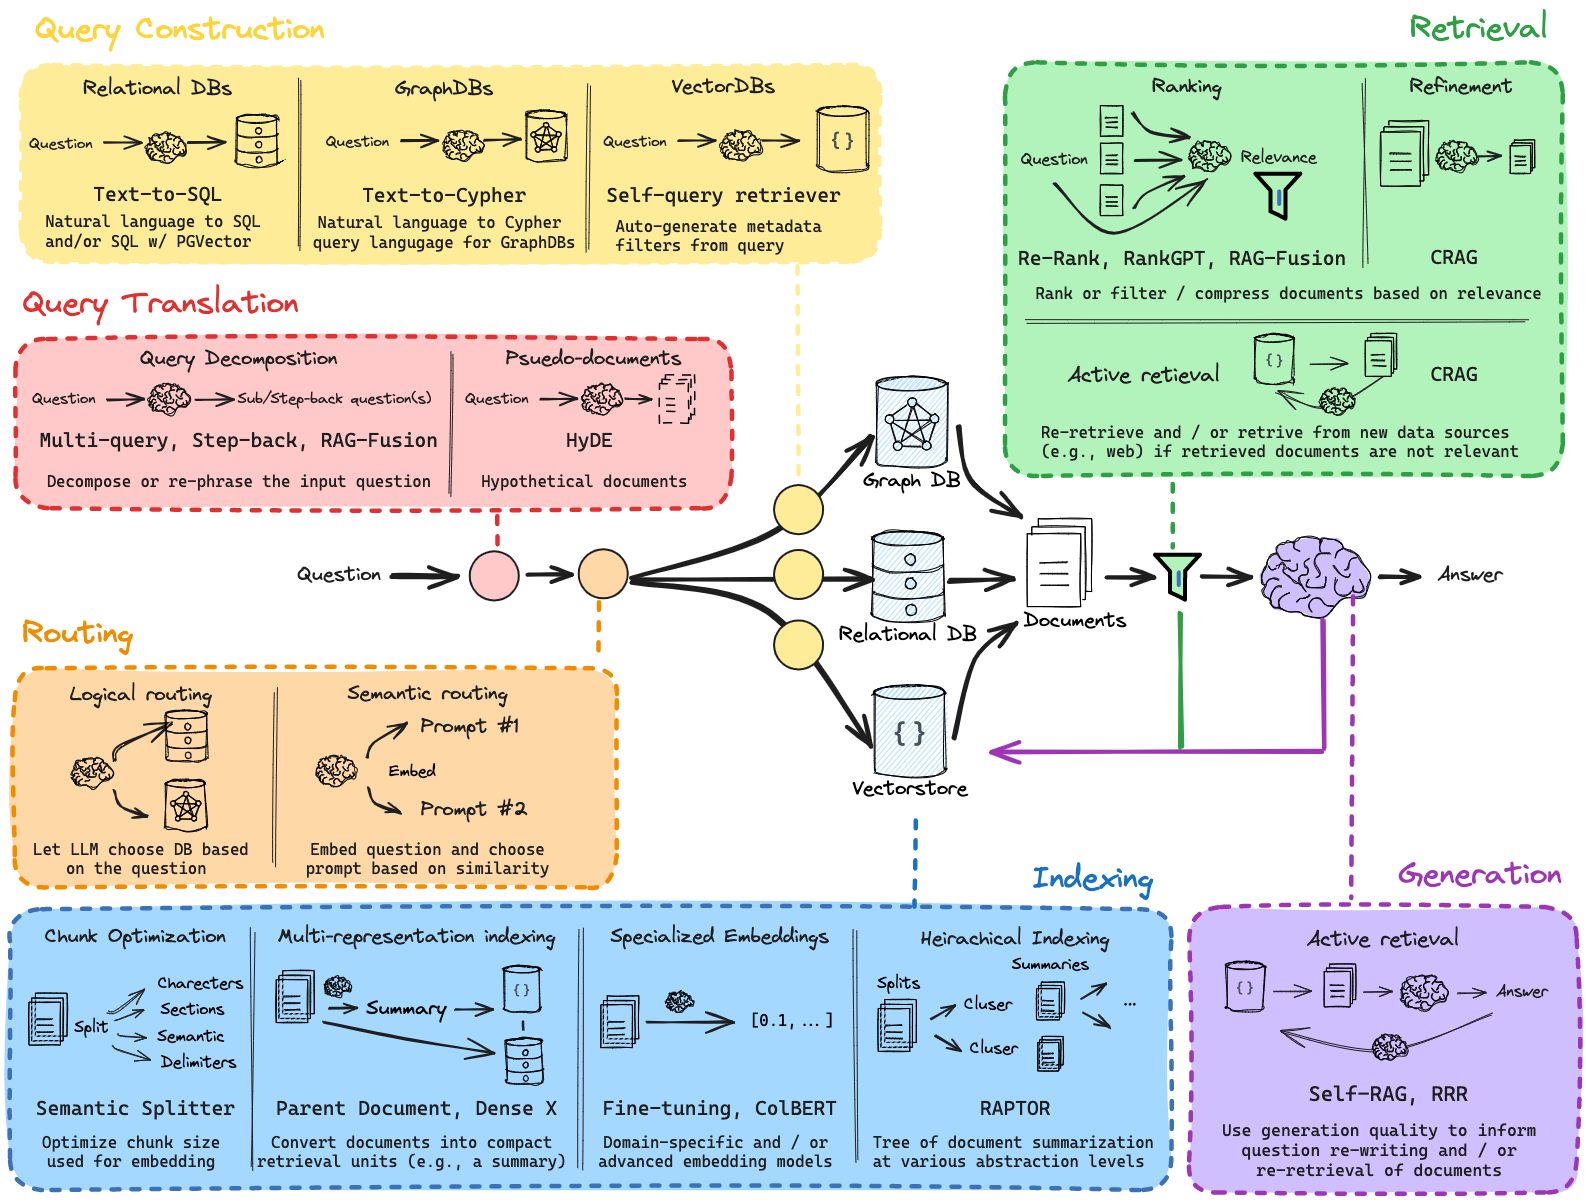
\includegraphics[width=\textwidth]{Images/cap2/rag_workflow.png}
    \caption{Workflow di RAG \cite{ragworkflow}}
    \label{fig:rag_workflow}
\end{figure}
RAG è un'architettura altamente personalizzabile e flessibile che può essere adattata a diversi compiti e scenari, quindi, nonostante il suo funzionamento di base rimanga lo stesso in tutte le sue varianti, la sua implementazione pratica può variare notevolmente a seconda delle esigenze specifiche.

\subsection{RAG passo dopo passo}
Analizziamo ora il funzionamento di RAG passo dopo passo (vedi \figurename{~\ref{fig:rag_workflow}}):

\subsubsection{Indexing}
Questa fase è presente in tutte le implementazioni di RAG e si tratta di una procedura che viene eseguita prima dell'avvio dell'architettura stessa. Serve a caricare i documenti della knowledge base all'interno di uno o più database in modo da renderli facilmente accessibili al retriever. Si può procedere in vari modi, ma solitamente si inizia effettuando un chunking dei dati e poi si procede con l'indicizzazione dei documenti. L'indicizzazione può essere fatta in maniera differente, a seconda del tipo di database utilizzato e a seconda dell'utilizzo che si deve fare dei documenti stessi. In particolare, per un database relazionale, si utilizza un'indicizzazione basata su chiavi primarie e chiavi esterne, mentre per un database vettoriale (vedi Paragrafo \ref{subsec:database_vettoriale}) si utilizza un'indicizzazione basata su vettori di embeddings. In aggiunta, è possibile utilizzare tecniche di indicizzazione più avanzate, come quella basata su grafi (ad esempio tramite Neo4j \cite{neo4j}) per ottenere implementazioni più efficienti e performanti. Quest'ultima tipologia è molto utile quando si vuole creare un sistema di indici gerarchici, vale a dire, un sistema in cui i documenti sono organizzati in una struttura ad albero o grafo che permette di accedere velocemente a documenti simili o correlati \cite{forer2024inferringscientificcrossdocumentcoreference}.

\subsubsection{Query Translation}
Si tratta della prima fase di elaborazione dell'input, ma non sempre viene implementato. Quando questo modulo viene utilizzato, la query dell'utente viene tradotta in una equivalente nel significato ma più adatta per il retriever. Questo passaggio è particolarmente utile quando il linguaggio utilizzato dal modello è diverso da quello della knowledge base. Ad esempio, se esso è addestrato in inglese ma la knowledge base è in italiano, la query dell'utente deve essere tradotta in inglese prima di essere passata al retriever. In questo passo è anche possibile che la query venga suddivisa in sotto-queries più specifiche per migliorare la precisione del retriever e per permettere al modello di rispondere a domande più complesse.

\subsubsection{Routing}
Il modulo di routing è responsabile della selezione del retriever più adatto per la query in ingresso. In generale, un sistema RAG può utilizzare diversi retriever, ognuno specializzato in un determinato tipo di query o di knowledge base. Il modulo di routing si occupa di identificare il retriever più adatto per la query in ingresso e di passare la query a tale retriever per il recupero dei documenti rilevanti. Questo modulo si occupa anche di decidere quale prompt utilizzare per il generatore in base ai risultati del retriever o alla natura della query. Ovviamente, il routing può essere implementato in modi diversi a seconda delle esigenze specifiche del sistema ma non è necessario se il sistema utilizza un solo retriever o se la gestione dei prompt è delegata ad un altro modulo o non è, anch'essa, necessaria.

\subsubsection{Query Construction}
Questa fase è presente in tutte le implementazioni di RAG e consiste nella costruzione della query da passare al retriever. La query può essere costruita in diversi modi a seconda delle esigenze specifiche del sistema, ma in generale, deve essere progettata in modo da massimizzare la precisione e la completezza del recupero dei documenti rilevanti. Inoltre, la query deve essere progettata in modo da massimizzare la coerenza e la coesione del testo generato dal modello. Si deve tenere presente che i documenti che verranno recuperati dal retriever si trovano dentro database di vario tipo, come database vettoriali, database relazionali, database di grafi, ecc. e quindi la query costruita deve essere compatibile con il tipo di database utilizzato.

\subsubsection{Retrieval}
È la fase cardine di RAG e consiste nel recupero effettivo dei documenti. Il retriever utilizza la query costruita nella fase precedente per recuperare i documenti rilevanti dalla knowledge base. Le informazioni recuperate possono essere di molteplici tipologie, da dati testuali (articoli, libri, pagine web, codice, ecc.) a contenuti multimediali (audio, foto, video ecc.). Il modo in cui recupera i documenti dipende dal tipo di database utilizzato e a seguito del recupero, i documenti possono essere restituiti integralmente al modello o subire ulteriori elaborazioni. Ad esempio, i documenti possono essere filtrati, ordinati, aggregati, ecc. prima di essere passati al generatore \cite{liu2023lostmiddlelanguagemodels}.

\subsubsection{Generation}
La fase finale consiste nell'elaborazione da parte della rete dei dati ricevuti in input (prompt di sistema, query dell'utente, documenti recuperati, ecc.) per generare la risposta finale. Il generatore può essere un qualsiasi LLM pre-addestrato, ma può anche essere un modello addestrato specificamente per il compito di generazione di testo. Il generatore utilizza le informazioni contenute nei documenti recuperati per generare una risposta accurata e coerente alla query dell'utente. La risposta generata può essere di vario tipo, da un semplice testo a una tabella, un grafico, un'immagine, ecc. Spesso è conveniente utilizzare varianti di LLM di tipo IT (Instruction Tuning) \cite{zhang2024instructiontuninglargelanguage,ouyang2022traininglanguagemodelsfollow} poiché riescono a generare risposte strutturate e più coerenti quando rispondono a domande basate su istruzioni specifiche ("Spiega perché...", "Riassumi questo...", "Traduci questa frase...").
Recenti studi hanno evidenziato che l'utilizzo di modelli LLM di piccole dimensioni \cite{hsieh2023distillingstepbystepoutperforminglarger,mukherjee2023orcaprogressivelearningcomplex} all'interno di architetture RAG può portare ad avere un sistema più rapido ma al tempo stesso molto accurato e coerente (ad esempio FLARE \cite{jiang2023activeretrievalaugmentedgeneration}).

\subsection{Database Vettoriale}
\label{subsec:database_vettoriale}
Per la realizzazione del progetto, che verrà introdotto nel Capitolo \ref{cap:omnibot1}, è stato utilizzato un database vettoriale per memorizzare i documenti della knowledge base. Un database vettoriale (detto anche VectorStore) memorizza i dati sotto forma di vettori, dove ogni documento o dato non strutturato è rappresentato tramite un embedding, ovvero un vettore di numeri reali.

Gli embeddings sono ottenuti tramite tecniche di machine learning che trasformano testi, immagini o audio in rappresentazioni numeriche dense, catturando così la semantica o le caratteristiche salienti dei dati.
Questa tipologia di database è particolarmente adatta per gestire dati non strutturati, poiché consente di effettuare operazioni di recupero e ricerca basate sulla similarità tra vettori. In un sistema del genere, il retriever può confrontare rapidamente la query dell'utente con i documenti presenti nella knowledge base, restituendo quelli più rilevanti grazie alla vicinanza tra i rispettivi embeddings nello spazio vettoriale.

Nella versione più recente del progetto, gli embeddings sono stati ottenuti utilizzando un modello di tipo Sentence Transformer dell'azienda Cohere. Questo, denominato \textit{"embed-multilingual-v3.0"} \cite{cohereembed} è stato addestrato su un corpus di testi molto ampio e diversificato, in modo da catturare le relazioni semantiche tra le parole e i concetti. Gli embeddings generati da questo embedder hanno dimensione 1024 e sono in grado di catturare le relazioni semantiche tra i documenti in modo efficace e accurato.
Quindi, appena un documento viene caricato nel database vettoriale, le sue features più significative vengono codificate in un vettore di dimensione 1024 che rappresenta il documento nello spazio vettoriale. Si può visualizzare lo spazio vettoriale come un'astrazione matematica in cui i documenti sono rappresentati come punti e la distanza tra i punti rappresenta la similarità tra i documenti. In questo modo, il retriever può confrontare la query dell'utente con i documenti presenti nel database e restituire quelli più rilevanti in base alla vicinanza tra i rispettivi embeddings.

\subsubsection{Visualizzazione di uno Spazio Vettoriale}
Per poter visualizzare graficamente i documenti nello spazio vettoriale, è possibile utilizzare tecniche di riduzione della dimensionalità, come la Principal Component Analysis (PCA) \cite{MACKIEWICZ1993303} o la t-Distributed Stochastic Neighbor Embedding (t-SNE) \cite{cai2022theoreticalfoundationstsnevisualizing,roy2024trustworthydimensionalityreduction}, che proiettano i vettori in uno spazio a dimensioni ridotte (ad esempio bidimensionale o tridimensionale), permettendo di visualizzare i documenti in un grafico.
Questo tipo di visualizzazione è particolarmente utile per capire come i documenti sono distribuiti nello spazio vettoriale e per identificare eventuali cluster o pattern nascosti nei dati.

Nello specifico verrà utilizzata la tecnica t-SNE poiché è più adatta a visualizzare dati non lineari e a catturare le relazioni semantiche tra i documenti.
Quest'ultima trasforma le distanze in probabilità per preservare le relazioni locali e utilizza una distribuzione t di Student per ridurre la dimensionalità in modo non lineare. In questo caso, la preservazione delle relazioni locali, porta a mantenere i punti vicini nei dati originali vicini anche nel nuovo spazio ridotto.
Si tratta di un approccio più diretto rispetto a quello della PCA che trovando le direzioni (componenti principali) lungo le quali i dati variano di più, riduce la dimensionalità mantenendo il più possibile la varianza originale dei dati.
Di seguito è riportato un frammento di codice Python che mostra come utilizzare la libreria scikit-learn per applicare la tecnica t-SNE \cite{scikittsne} a un insieme di vettori multidimensionali:
\begin{lstlisting}[label=lst:tsne, caption={Esempio applicazione t-SNE}]  
from sklearn.manifold import TSNE
from sklearn.preprocessing import LabelEncoder
from vectordb import VectorDatabase

vectorstore = VectorDatabase.load_from_local(*@\textcolor{functionyellow}{(}@*)"path/to/db"(*@\textcolor{functionyellow}{)}@*)
vectors = vectorstore.get_vectors(*@\textcolor{functionyellow}{()}@*)
labels = vectorstore.get_labels(*@\textcolor{functionyellow}{()}@*)

tsne = TSNE(*@\textcolor{functionyellow}{(}@*)n_components=(*@\textcolor{numberyellow}{3}@*), perplexity=(*@\textcolor{numberyellow}{50}@*)(*@\textcolor{functionyellow}{)}@*)
label_encoder = LabelEncoder(*@\textcolor{functionyellow}{()}@*)

vectors_3d = tsne.fit_transform(*@\textcolor{functionyellow}{(}@*)vectors(*@\textcolor{functionyellow}{)}@*)
encoded_labels = label_encoder.fit_transform(*@\textcolor{functionyellow}{(}@*)labels(*@\textcolor{functionyellow}{)}@*)

# (*@\textcolor{commentsgreen}{...}@*)
\end{lstlisting}
Una volta applicato l'algoritmo t-SNE, è possibile visualizzare i documenti nello spazio tridimensionale utilizzando una libreria di visualizzazione.
\begin{figure}[!t]
    \centering
    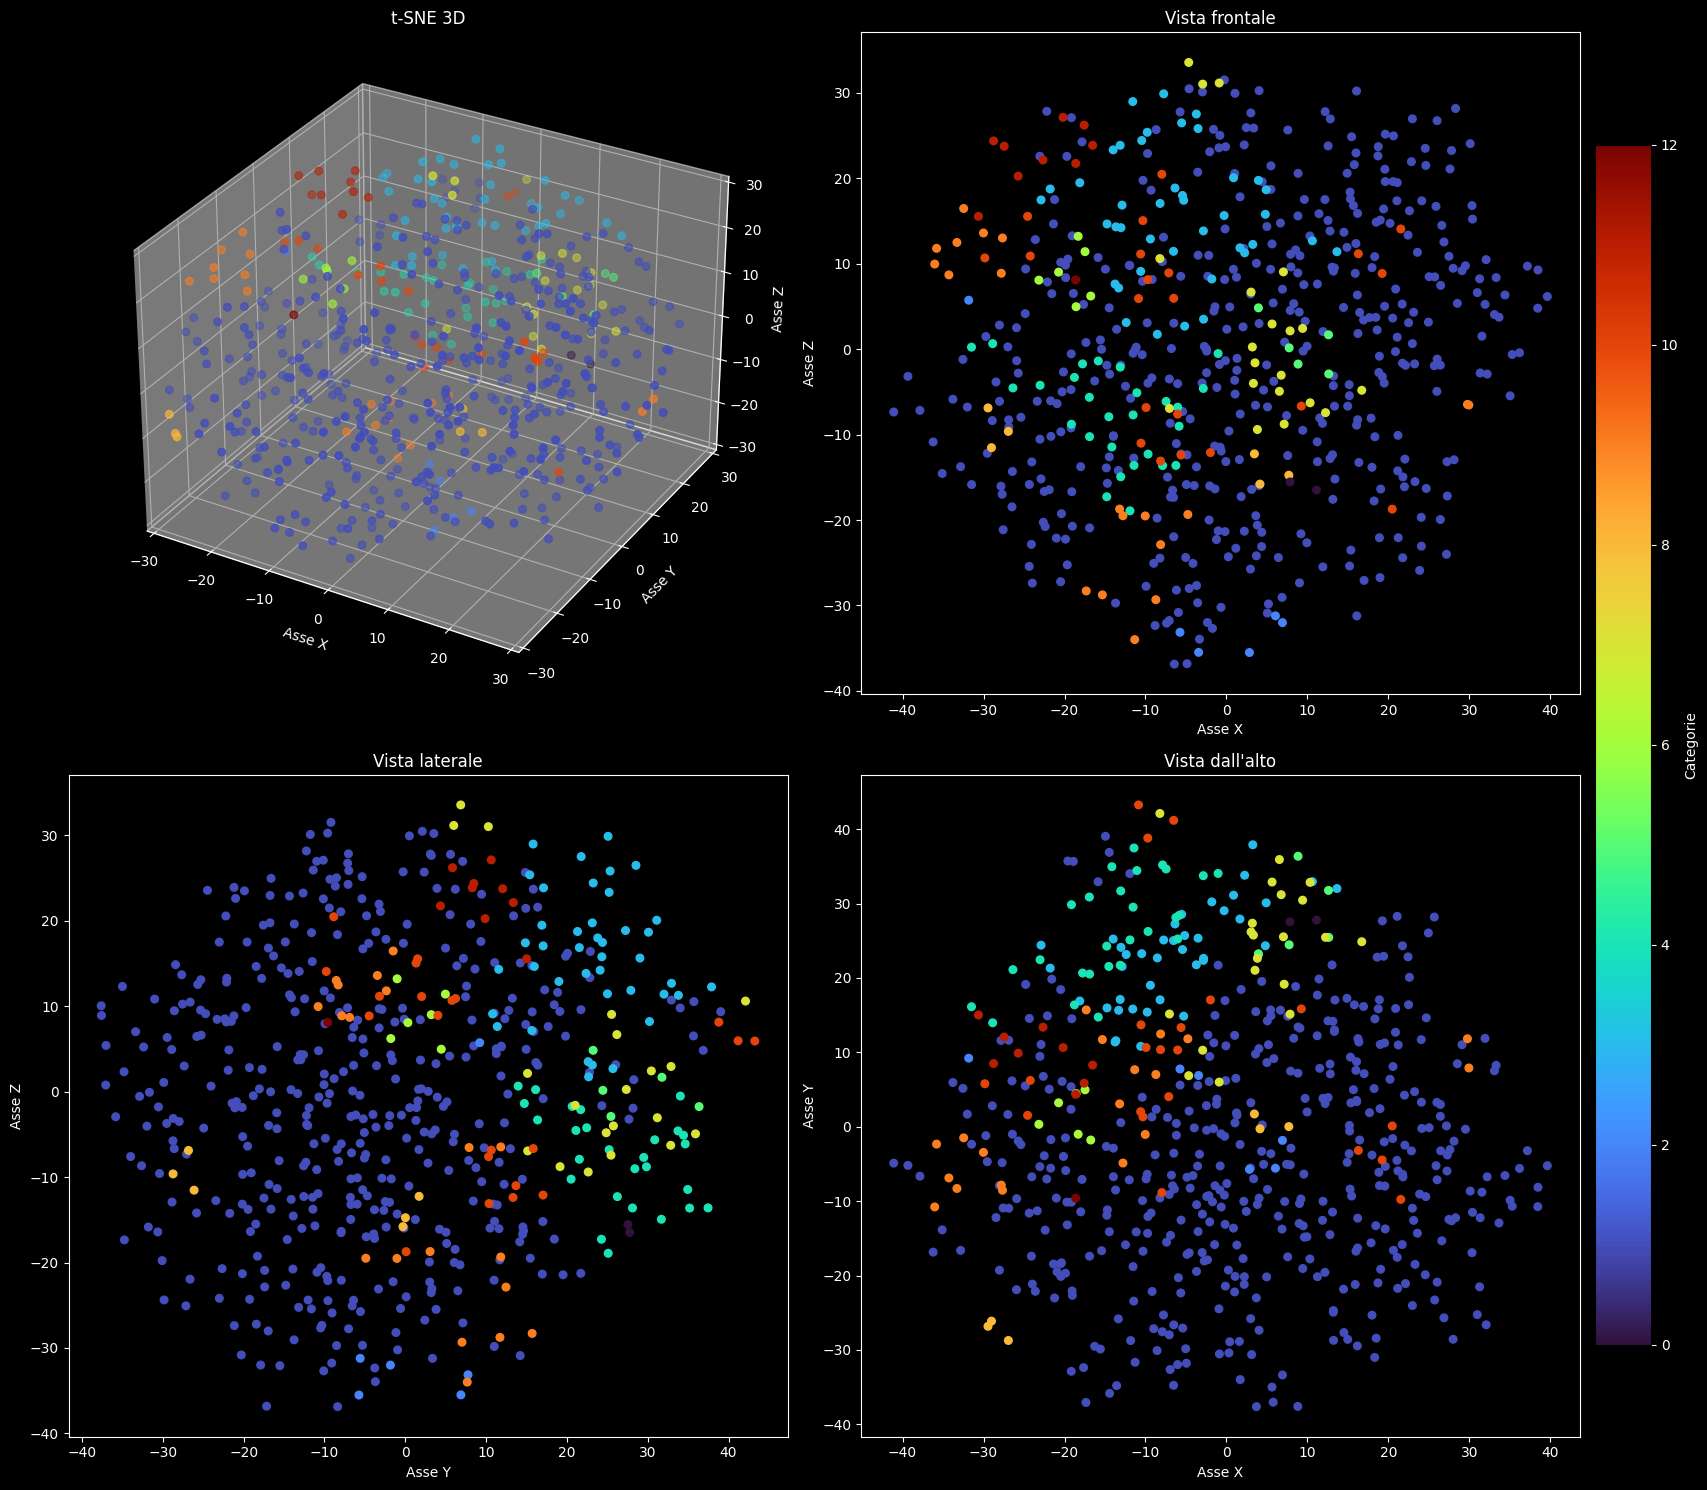
\includegraphics[width=\textwidth]{Images/cap2/nero.png}
    \caption{Visualizzazione di un database vettoriale tramite t-SNE}
    \label{fig:databse_vettoriale}
\end{figure}

Il grafico riportato in \figurename{~\ref{fig:databse_vettoriale}} è stato realizzato tramite la libreria Matplotlib e rappresenta tutti i documenti del database vettoriale come punti in uno spazio tridimensionale. Ogni punto ha un colore che è diverso a seconda della classe di appartenenza del documento stesso. Si può notare che molti punti dello stesso colore si riuniscono in aree ben distinte, suggerendo la presenza di cluster o gruppi di documenti simili tra loro. Più un punto è vicino ad un altro, più i due documenti corrispondenti sono simili tra loro. Naturalmente non è detto che punti vicini siano necessariamente dello stesso colore, infatti capita che documenti di classi differenti parlino di uno stesso argomento (anche se in modo diverso) e quindi siano vicini nello spazio vettoriale.
\subsection{Retriever Vettoriale}
Il retriever di un database vettoriale può essere implementato ed utilizzato in molti modi, il modo specifico in cui è stato implementato per il progetto presentato in questa tesi verrà introdotto a partire dal Capitolo \ref{cap:omnibot1}. In generale, un retriever vettoriale funziona confrontando la query dell'utente con i documenti presenti nel database e restituendo quelli più simili alla query in base alla vicinanza tra i rispettivi embeddings.

Dunque, per effettuare la ricerca, è prima necessario calcolare l'embedding della query dell'utente. Una volta fatto ciò si torna in output il documento, o meglio, una lista di documenti, più simili alla query. Si possono effettuare anche ricerche a partire da altri documenti stessi, in questo caso si calcola l'embedding del documento e si restituiscono i documenti più simili a quello in input.

Ci sono diverse tipologie di ricerche, le più comuni sono:
\begin{itemize}
    \item \textbf{Ricerca per similarità semantica}: Si cerca di trovare i documenti più simili alla query in base alla vicinanza tra i rispettivi embeddings.
    \item \textbf{Maximal Marginal Relevance (MMR)}: Si cerca di trovare i documenti più simili alla query ma che siano anche diversi tra loro. Questo approccio è utile per evitare la ripetizione di informazioni simili nei documenti restituiti.
\end{itemize}
Dopo ciascuna di queste ricerche è possibile applicare dei filtri di similarità o distanza che permettono di eliminare dall'output del retriever eventuali documenti non abbastanza simili alla query e quindi potenzialmente non rilevanti. Solitamente similarità o distanza vengono forniti tra i metadati dell'output del retriever (a seconda che la ricerca si basi sulla similarità o sulla distanza da embeddings noti) e assumono valori che vengono interpretati in maniera opposta: più è alto il valore di similarità (di solito tra 0 e 1), allora, più è basso il valore di distanza e viceversa. Solitamente la similarità si calcola utilizzando la \textit{Cosine Similarity}, mentre la distanza si calcola utilizzando la \textit{Euclidean Distance} o la \textit{Manhattan Distance}.
\begin{align}
    \text{Cosine Similarity} &= \frac{A \cdot B}{\|A\| \|B\|} \\
    \text{Euclidean Distance} &= \sqrt{\sum_{i=1}^{n} (A_i - B_i)^2} \\
    \text{Manhattan Distance} &= \sum_{i=1}^{n} |A_i - B_i|
\end{align}

\subsection{Tecniche di Prompt Engineering in RAG}
Il Prompt Engineering \cite{Beurer_Kellner_2023} è una tecnica che consiste nella progettazione di prompt specifici per guidare il modello nella generazione di testo. Questa tecnica è particolarmente utile quando si vuole controllare il comportamento dello stesso e indirizzarlo verso una determinata risposta. Nel contesto di RAG, il Prompt Engineering è utilizzato per guidare il generatore nella generazione di risposte accurate e coerenti, utilizzando le informazioni contenute nei documenti recuperati dal retriever. In un certo senso l'architettura RAG stessa è una forma di Prompt Engineering, poiché il retriever fornisce al generatore le informazioni necessarie per generare una risposta corretta. Praticamente l'LLM riceverà in input sia la query che la risposta ad essa. Tuttavia, è possibile utilizzare tecniche di Prompt Engineering più avanzate per migliorare ulteriormente le prestazioni del modello e per indirizzarlo verso risposte più precise. Ad esempio, si possono utilizzare prompt specifici per guidare il generatore nella generazione di risposte strutturate o per indirizzarlo verso risposte più lunghe e dettagliate. In particolare, si possono utilizzare prompt di sistema per fornire al modello informazioni aggiuntive sul contesto della conversazione o per guidarlo nella generazione di risposte di qualità superiore e maggiormente pertinenti.

Un esempio di prompt di sistema è il seguente:
\begin{lstlisting}[label=lst:prompt, caption={Esempio di prompt di sistema}, literate={.}{{\textcolor{stringbrown}{.}}}1 {,}{{\textcolor{stringbrown}{,}}}1 {=}{{\textcolor{white}{=}}}1]
RAG_PROMPT = (*@\textcolor{stringbrown}{"""Tu sei un assistente virtuale che aiuta}@*)
                (*@\textcolor{stringbrown}{gli utenti rispondendo alle loro domande.}@*)
                (*@\textcolor{stringbrown}{Rispondi nella stessa lingua della domanda.}@*)
                (*@\textcolor{stringbrown}{NON ripetere la domanda dell'utente.}@*)
                (*@\textcolor{stringbrown}{Rispondi con tono formale e professionale.}@*)
                (*@\textcolor{stringbrown}{Se non sai rispondere alla domanda, puoi}@*)
                (*@\textcolor{stringbrown}{dire "Non lo so".}@*)
                (*@\textcolor{stringbrown}{Puoi usare le informazioni contenute nei}@*)
                (*@\textcolor{stringbrown}{seguenti documenti:}@*)
                (*@\textcolor{defblue}{\{context\}}@*)
                
                (*@\textcolor{stringbrown}{Domanda:}@*)
                (*@\textcolor{defblue}{\{query\}}@*)(*@\textcolor{stringbrown}{"""}@*)
\end{lstlisting}
I campi \{context\} e \{query\} vengono riempiti con le informazioni recuperate dal retriever e con la query dell'utente, rispettivamente. In questo modo, il modello riceve in input tutte le informazioni necessarie per generare una risposta accurata e che sia compatibile con la domanda dell'utente. Inoltre, il prompt di sistema fornisce al generatore istruzioni dettagliate su come rispondere alla domanda e su come utilizzare le informazioni contenute nei documenti recuperati dal retriever.

\section{Perché RAG?}
RAG è uno strumento molto potente se integrato con un LLM, poiché permette di aggiungere conoscenze esterne migliorando la qualità delle risposte generate. Ma RAG è davvero la soluzione definitiva per risolvere tutte le limitazioni degli LLM? La risposta è no. Pur essendo efficace in molti contesti, ha alcuni difetti e limitazioni. In più, lo sviluppo di tecniche e modelli più sofisticati, insieme all'integrazione di framework all'avanguardia, sta lentamente spingendo RAG ai margini. Esaminiamo nel dettaglio le alternative e cerchiamo di rispondere alla domanda "Perché RAG?" in modo più approfondito.

\subsection{Alternative a RAG}
Esistono diverse metodologie per migliorare e personalizzare un modello linguistico, ciascuna con vantaggi e limitazioni specifiche. Tra queste, possiamo identificare:
\begin{itemize}
    \item \textbf{Fine Tuning}: Questa è una delle tecniche più comuni per personalizzare un LLM \cite{lu2024finetuninglargelanguagemodels}. Consiste nel riaddestrare il modello su un dataset specifico dopo l'addestramento originale, adattandone i parametri alle nuove esigenze.
        \begin{itemize}
            \item \textbf{Vantaggi}: Il modello diventa più accurato e specializzato per un determinato dominio.
            \item \textbf{Svantaggi}: Richiede elevate risorse computazionali e di tempo, oltre a grandi quantità di dati. È inoltre poco flessibile quando le informazioni devono essere aggiornate frequentemente.
        \end{itemize}
    \item \textbf{Instruction Tuning}: In questo caso, si adatta il comportamento del modello affinché segua meglio istruzioni in linguaggio naturale \cite{ouyang2022traininglanguagemodelsfollow}. Si basa sull'addestramento su compiti eterogenei, per migliorare la risposta a prompt strutturati sotto forma di istruzioni esplicite.
        \begin{itemize}
            \item \textbf{Vantaggi}: Migliora la capacità dell'LLM di affrontare diversi task attraverso prompt più complessi.
            \item \textbf{Svantaggi}: Sebbene ottimizzi le risposte, non aggiunge nuove informazioni e non risolve il problema dell'obsolescenza della conoscenza del modello.
        \end{itemize}
    \item \textbf{Prompt Tuning}: Questa tecnica si basa sull'ottimizzazione dei prompt per ottenere risposte migliori da un LLM pre-addestrato, senza modificarne i parametri interni. Il focus è sulla formulazione delle richieste in modo tale da sfruttare al massimo le conoscenze preesistenti del modello.
        \begin{itemize}
            \item \textbf{Vantaggi}: È computazionalmente efficiente, non richiede riaddestramento e può essere facilmente adattata a diversi contesti.
            \item \textbf{Svantaggi}: Non consente l'aggiunta di nuove informazioni, ma si limita a migliorare l'uso di quelle già presenti nel modello.
        \end{itemize}
    \item \textbf{LLM Agents}: Gli agenti basati su LLM estendono le capacità del modello linguistico con sistemi di esecuzione di task \cite{llmagents}. Questi agenti possono eseguire operazioni complesse, come navigare sul web o prendere decisioni basate su input dinamici.
        \begin{itemize}
            \item \textbf{Vantaggi}: Estendono l'applicabilità del prodotto oltre la generazione di testo, integrando capacità di esecuzione pratica.
            \item \textbf{Svantaggi}: Richiedono l'integrazione con sistemi complessi e, spesso, non sono orientati all'aggiunta di nuove conoscenze nel modello stesso.
        \end{itemize}
\end{itemize}

\subsection{RAG vs tutti}
RAG è la tecnica più adatta quando si vuole aggiornare la base di conoscenza di un LLM, senza richiedere un riaddestramento completo o un uso intensivo di risorse computazionali. A differenza delle altre tecniche, che mirano principalmente a modificare il comportamento del modello o a migliorare l'interazione con esso, RAG permette di integrare nuove informazioni esterne in modo dinamico \cite{ragandfine}.

Perché RAG? La risposta è semplice: è il metodo migliore per aggiungere informazioni nuove a un LLM senza la necessità di riaddestrarlo, offrendo così un aggiornamento della conoscenza in modo rapido ed efficiente. Tuttavia, non è la soluzione ideale per specializzare il modello o per fargli eseguire compiti complessi.
Il compromesso ottimale è l'integrazione di RAG con altre tecniche \cite{lewis2021retrievalaugmentedgenerationknowledgeintensivenlp,zhao2024retrievalaugmentedgenerationrag}. Ad esempio, una combinazione con agenti LLM o tecniche di modifica della catena di pensiero (chain-of-thoughts) può ampliare ulteriormente le capacità del modello, portando a risultati più precisi e articolati.
In conclusione, mentre RAG si distingue per la sua capacità di integrare informazioni esterne in modo rapido e senza costi computazionali eccessivi, il suo vero potenziale emerge quando viene combinato con altre tecniche per ottenere un LLM che sia informato e performante.

\chapter{OmniBot: L'inizio}
\label{cap:omnibot1}
L'iter di ricerca e sviluppo che ha condotto alla creazione di OmniBot, un assistente conversazionale basato sull'architettura RAG, ha seguito un percorso dettagliato per garantire supporto all'utente in un'ampia gamma di attività. In questo capitolo vengono analizzate le fasi iniziali del progetto, con un approfondimento sulle difficoltà e sui problemi affrontati, nonché sulle scelte progettuali e tecnologiche che hanno guidato la realizzazione di un prototipo funzionante.

\subsubsection{L'obiettivo}
L'obiettivo del progetto di tirocinio, sviluppato per un cliente dell'azienda Intellisync \cite{intellisync}, consisteva nel creare un chatbot capace di rispondere a domande su argomenti estremamente specifici, probabilmente non inclusi nelle conoscenze di un modello di linguaggio pre-addestrato. Inoltre, tra i requisiti fondamentali era richiesto che l'intero sistema funzionasse in locale, evitando così la necessità di effettuare richieste a server remoti.

\section{Alla Ricerca di un LLM}
\label{sec:ricercallm}
Il primo passo consisteva nella scelta di un modello di piccole dimensioni, in modo che potesse essere eseguito direttamente sul computer, tenendo conto che le risorse maggiormente richieste da un LLM sono memoria, CPU e GPU. Il computer utilizzato, un Acer Aspire 7 A715-42G, offriva le seguenti specifiche:
\begin{itemize}
    \item \textbf{Memoria RAM}: 16 GB DDR4
    \item \textbf{CPU}: Ryzen 7 5700U
    \item \textbf{GPU}: NVIDIA GeForce RTX 3050 Laptop da 4 GB
\end{itemize}
Per garantire un'esperienza utente fluida, era essenziale che il modello fosse in grado di rispondere rapidamente, richiedendo che potesse essere caricato integralmente, o quasi, nella VRAM della GPU. Considerati questi requisiti, la ricerca di un LLM adatto è stata avviata sulla piattaforma \textit{Hugging Face} \cite{huggingfacehomepage}.

\subsection{Hugging Face}
Hugging Face è un hub di modelli (non solo di NLP), dataset, tokenizzatori e numerosi altri strumenti di pubblica utilità. La piattaforma offre una vasta gamma di prodotti, per la maggior parte open-source, quindi liberamente scaricabili e utilizzabili. I modelli disponibili variano notevolmente per dimensioni, spaziando da soluzioni più leggere di pochi MB fino a modelli di diverse decine di TB. Inizialmente, è stata considerata la possibilità di utilizzare \textit{Gemma2-2B-IT}, uno dei modelli sviluppati da Google \cite{gemma22bit}.

\subsubsection{Gemma2-2B-IT}
Il modello, con 2.61 miliardi di parametri, era suddiviso in due file di tipo safetensors, un formato che gestisce dati tensoriali (matrici multidimensionali di valori float a precisione variabile) applicando checksum e cifrature. La dimensione complessiva dei file ammontava a 5.5 GB, risultando quindi superiore alla capacità della VRAM disponibile. Sebbene Hugging Face offra API per eseguire i modelli anche in remoto, si è scelto di scaricarlo ed eseguirlo in locale, evitando richieste a server esterni. I modelli possono essere scaricati in diversi modi da Hugging Face, ad esempio tramite un'API dedicata, o con il comando \textit{"huggingface-cli"} o direttamente dalla pagina della repository del modello. Nel caso specifico, è stata utilizzata la libreria \textit{transformers} di Hugging Face per il download di Gemma2.
\begin{lstlisting}[label=lst:gemma2, caption={Installazione di Gemma2}]
from transformers import AutoTokenizer, AutoModelForCausalLM
import torch

model_name = (*@\textcolor{stringbrown}{"google/gemma-2-2b-it"}@*)
tokenizer = AutoTokenizer.from_pretrained(*@\textcolor{functionyellow}{(}@*)model_name(*@\textcolor{functionyellow}{)}@*)
model = AutoModelForCausalLM.from_pretrained(*@\textcolor{functionyellow}{(}@*)
    model_name,
    device_map="auto",
    torch_dtype=torch.bfloat16,
(*@\textcolor{functionyellow}{)}@*)
\end{lstlisting}
Il codice in Codice \ref{lst:gemma2} scarica il modello Gemma2-2B-IT e lo carica in memoria. Esso è stato memorizzato con il tipo di dato "bfloat16", che è una tipologia di dato a precisione ridotta, che permette di ridurre la memoria necessaria per memorizzare i pesi del modello. Il bfloat16 è supportato solo da alcune GPU, tra cui l'RTX 3050 a disposizione.

Il passo successivo consisteva nell'effettuare dei test, per vedere se fosse effettivamente in grado di rispondere a domande in maniera coerente e se riuscisse a farlo in tempi brevi.
\begin{lstlisting}[label=lst:gemma2test, caption={Primo test di Gemma2}]
input_text = "Write me a poem about Machine Learning(*@\textcolor{stringbrown}{.}@*)"
input_ids = tokenizer(*@\textcolor{functionyellow}{(}@*)
                      input_text, return_tensors="pt"
                     (*@\textcolor{functionyellow}{)}@*).to(*@\textcolor{functionyellow}{(}@*)"cuda"(*@\textcolor{functionyellow}{)}@*)

outputs = model.generate(*@\textcolor{functionyellow}{(}@*)(*@\textcolor{white}{**}@*)input_ids, max_new_tokens=(*@\textcolor{numberyellow}{32}@*)(*@\textcolor{functionyellow}{)}@*)
print(*@\textcolor{functionyellow}{(}@*)tokenizer.decode(*@\textcolor{keywordpurple}{(}@*)outputs(*@\textcolor{defblue}{[}@*)(*@\textcolor{numberyellow}{0}@*)(*@\textcolor{defblue}{]}@*)(*@\textcolor{keywordpurple}{)}@*)(*@\textcolor{functionyellow}{)}@*)
\end{lstlisting}
Il codice in Codice \ref{lst:gemma2test} genera un poema di 32 token a partire da un input testuale. Il modello, nonostante abbia generato un output di buona qualità, ha impiegato diversi minuti per generare il poema. L'output generato è stato il seguente:
\begin{center}
    \textit{"In silicon seas, a mind takes flight,} \\
    \textit{Learning patterns, bathed in data's light.} \\
    \textit{No flesh or bone, but algorithms bright,} \\
    \textit{Machine learning, a curious, elegant sight.} \\
    \textit{} \\
    \textit{From whispers of code, a thinking draw,} \\
    \textit{Trained on terabytes, fast and raw.} \\
    \textit{Be it images or text, a vast array,} \\
    \textit{Understanding the world, come what may.} \\
    \textit{} \\
    \textit{It sifts and categorizes, predicts the next,} \\
    \textit{A mastery of numbers, instinctively set"}
\end{center}

A quel punto si è provato a inviare lo stesso input, ma in lingua italiana. Tuttavia, dopo 15 minuti di attesa, l'output non era ancora stato generato. Ipotizzando che vi fosse un problema, è stato deciso di riprovare, aumentando il tempo di attesa. Dopo circa 25 minuti, l'output generato è stato il seguente:
\begin{center}
    \textit{"Il poema"}
\end{center}
Sono seguiti altri test, purtroppo Gemma2 non è mai riuscito a generare un output in lingua italiana in tempi brevi e con una qualità accettabile.

\subsubsection{Llama3-8B}
Dopo aver constatato che l'LLM sviluppato da Google non era adatto alle esigenze, è stata avviata la ricerca di un altro modello di dimensioni superiori. La scelta è ricaduta su \textit{Llama3}, un LLM sviluppato da Meta, disponibile in due versioni: una più piccola con 8 miliardi di parametri e una più grande con 70 miliardi di parametri. È stata scelta la versione più piccola, con un peso di circa 16 GB \cite{llama38b}.

Il modello è stato scaricato e caricato in memoria utilizzando le stesse funzioni impiegate per Gemma2-2B-IT. Tuttavia, questa volta sono stati utilizzati esclusivamente input in lingua italiana. Poiché Llama3 risultava essere più grande rispetto a Gemma2, è stato necessario attendere molto più a lungo per ottenere la prima risposta. Infatti, è stato necessario attendere ben 83 minuti prima di poter leggere la risposta, ma l'output generato a partire dall'input \textit{"Ciao, dimmi chi sei e se sai parlare in italiano"} è stato il seguente:
\begin{center}
    \textit{"Ciao, sono un modello di linguaggio addestrato da Meta. Sì, so parlare italiano. Come posso aiutarti oggi?"}
\end{center}
Nonostante l'output generato fosse di buona qualità, il tempo di attesa era troppo lungo per poter utilizzare Llama3 in un'applicazione in tempo reale.

\subsection{Ollama}
Era chiaro che per raggiungere l'obiettivo prefissato fosse necessario un modello di dimensioni modeste, ma allo stesso tempo tale modello richiedeva risorse di cui non si disponeva. Continuando la ricerca, è stato individuato \textit{Ollama} \cite{ollamasite, ollamagithub}, un gestore di modelli di NLP di varie dimensioni sviluppato da Meta. Ollama consente di eseguire modelli di dimensioni ridotte anche su hardware con risorse limitate, grazie all'adozione della tecnica della quantizzazione \cite{quantization}.

\subsubsection{Quantizzazione}
La quantizzazione è una tecnica utilizzata per ridurre il consumo di memoria e i requisiti computazionali nei modelli di machine learning, inclusi i Large Language Models (LLM). Questo viene ottenuto riducendo la precisione dei pesi e delle attivazioni della rete, rappresentando i numeri con meno bit rispetto alla rappresentazione a virgola mobile a 32 bit (FP32) standard.
Esistono vari tipi di quantizzazione e a seconda del tipo di quantizzazione utilizzata, si possono ottenere risultati diversi.
\begin{figure}[!t]
    \centering
    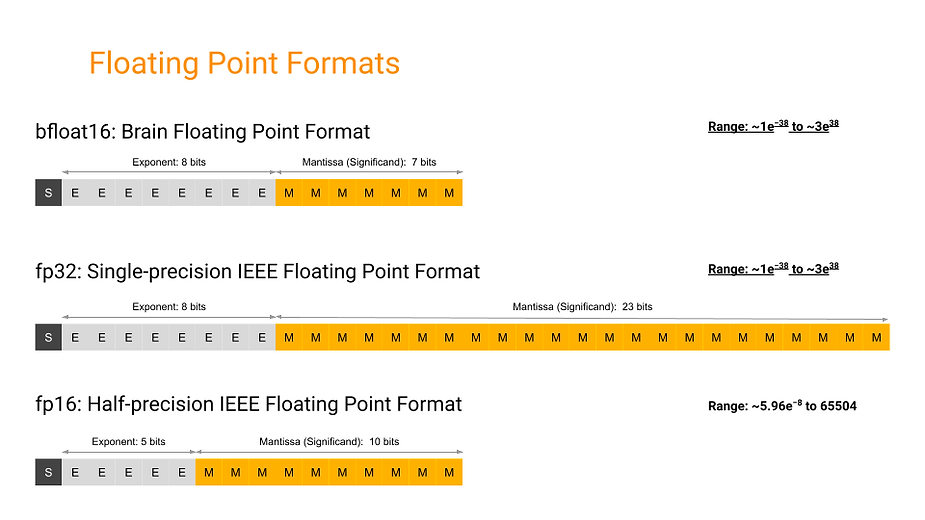
\includegraphics[width=\textwidth]{Images/cap3/quant.png}
    \caption{Formati di rappresentazione dei numeri a virgola mobile \cite{quanttensorops}}
    \label{fig:floatingpoint}
\end{figure}
I tipi di quantizzazione più comuni sono:
\begin{itemize}
    \item \textbf{INT8}: I pesi e le attivazioni vengono rappresentati con 8 bit, riducendo la memoria richiesta per memorizzare i pesi della rete e migliorando la velocità di esecuzione del modello.
    \item \textbf{FP16}: I pesi e le attivazioni contengono numeri a virgola mobile rappresentabili con 16 bit di cui 1 bit per il segno, 5 bit per l'esponente e 10 bit per la mantissa.
    \item \textbf{BF16}: Simile a FP16, ma con più bit dedicati all'esponente, utile per evitare perdite di precisione nelle reti profonde (questa è la quantizzazione usata con i modelli di Hugging Face, vedi Codice \ref{lst:gemma2}).
    \item \textbf{Qn[K S/M/L]}: I pesi e le attivazioni vengono rappresentati con n bit, ma a sua volta esistono varianti a seconda che vengano effettuate o meno delle correzioni sulla perplessità. In quel caso viene aggiunto il suffisso K e una misura di correzione (S/M/L).
\end{itemize}

\subsubsection{Llama3-8B-Q4}
Tornando a Ollama, il modello scelto è stato nuovamente Llama3 da 8B di parametri \cite{llama3ollama}, ma questa volta era disponibile una versione con quantizzazione Q4. Questo ha ridotto significativamente le dimensioni del modello, portandolo a un peso di soli 4.7 GB, rendendolo quindi compatibile con la capacità della VRAM della GPU a disposizione.

Ollama consente di scaricare i modelli disponibili utilizzando il semplice comando \textit{"ollama pull <nome-modello>"}. Successivamente, è possibile avviare una conversazione direttamente da terminale con il comando \textit{"ollama run <nome-modello>"}. Il modello ha fornito risposte in tempi rapidi (circa 1 secondo) e con una buona qualità in diverse lingue, tra cui l'italiano. Pertanto, è stato deciso di utilizzare Ollama per gestire i modelli di NLP all'interno del progetto.

\section{La RAG Chain}
Dopo aver selezionato l'LLM da utilizzare, la decisione successiva è stata quella di integrare la tecnologia RAG nel progetto. Per implementarla, è stato necessario sviluppare l'architettura che gestisse il passaggio dei dati rilevanti all'LLM. Le ricerche hanno condotto rapidamente alla scoperta di LangChain \cite{langchain}.

\subsection{LangChain}
LangChain è un framework di Intelligenza Artificiale che serve a gestire pipeline di elaborazione di modelli di NLP. Esso mette a disposizione numerosi strumenti che possono essere utili per gestire pressoché qualsiasi tipo di azione necessaria all'interno di un progetto di NLP. Questi strumenti spaziano da embedders, vectorstores, retrievers, fino ad arrivare a modelli o agenti.

Il cuore di LangChain è il concetto di "Chain", ovvero una sequenza di azioni che vengono eseguite in ordine. Queste catene possono essere caricate da esempi già pronti, oppure possono essere create da zero sfruttando le risorse messe a disposizione dalle librerie di LangChain.

Per iniziare, è stata creata una RAG Chain di base, in grado di eseguire una ricerca all'interno di un database di documenti e di passare il risultato all'LLM per la generazione di una risposta.

Il primo passo è stato la preparazione dei dati da inserire nel database vettoriale, che è stato possibile grazie ai seguenti elementi:
\begin{itemize}
    \item \textbf{Un Loader di documenti}: Un loader è un oggetto che prende in input dati in un formato specifico e li trasforma nel formato \textit{Document}. Questo formato è usato da LangChain per rappresentare i documenti e contiene due campi principali: \textit{page\textunderscore content}, contenente il testo del documento e \textit{metadata}, formato da un dizionario che contiene informazioni aggiuntive sul documento.
    \item \textbf{Uno Splitter}: Uno splitter è un oggetto che prende in input un Documento e lo divide in Documenti più piccoli. Questo è utile per dividere un testo lungo in paragrafi o frasi.
\end{itemize}
\begin{figure}[!t]
    \centering
    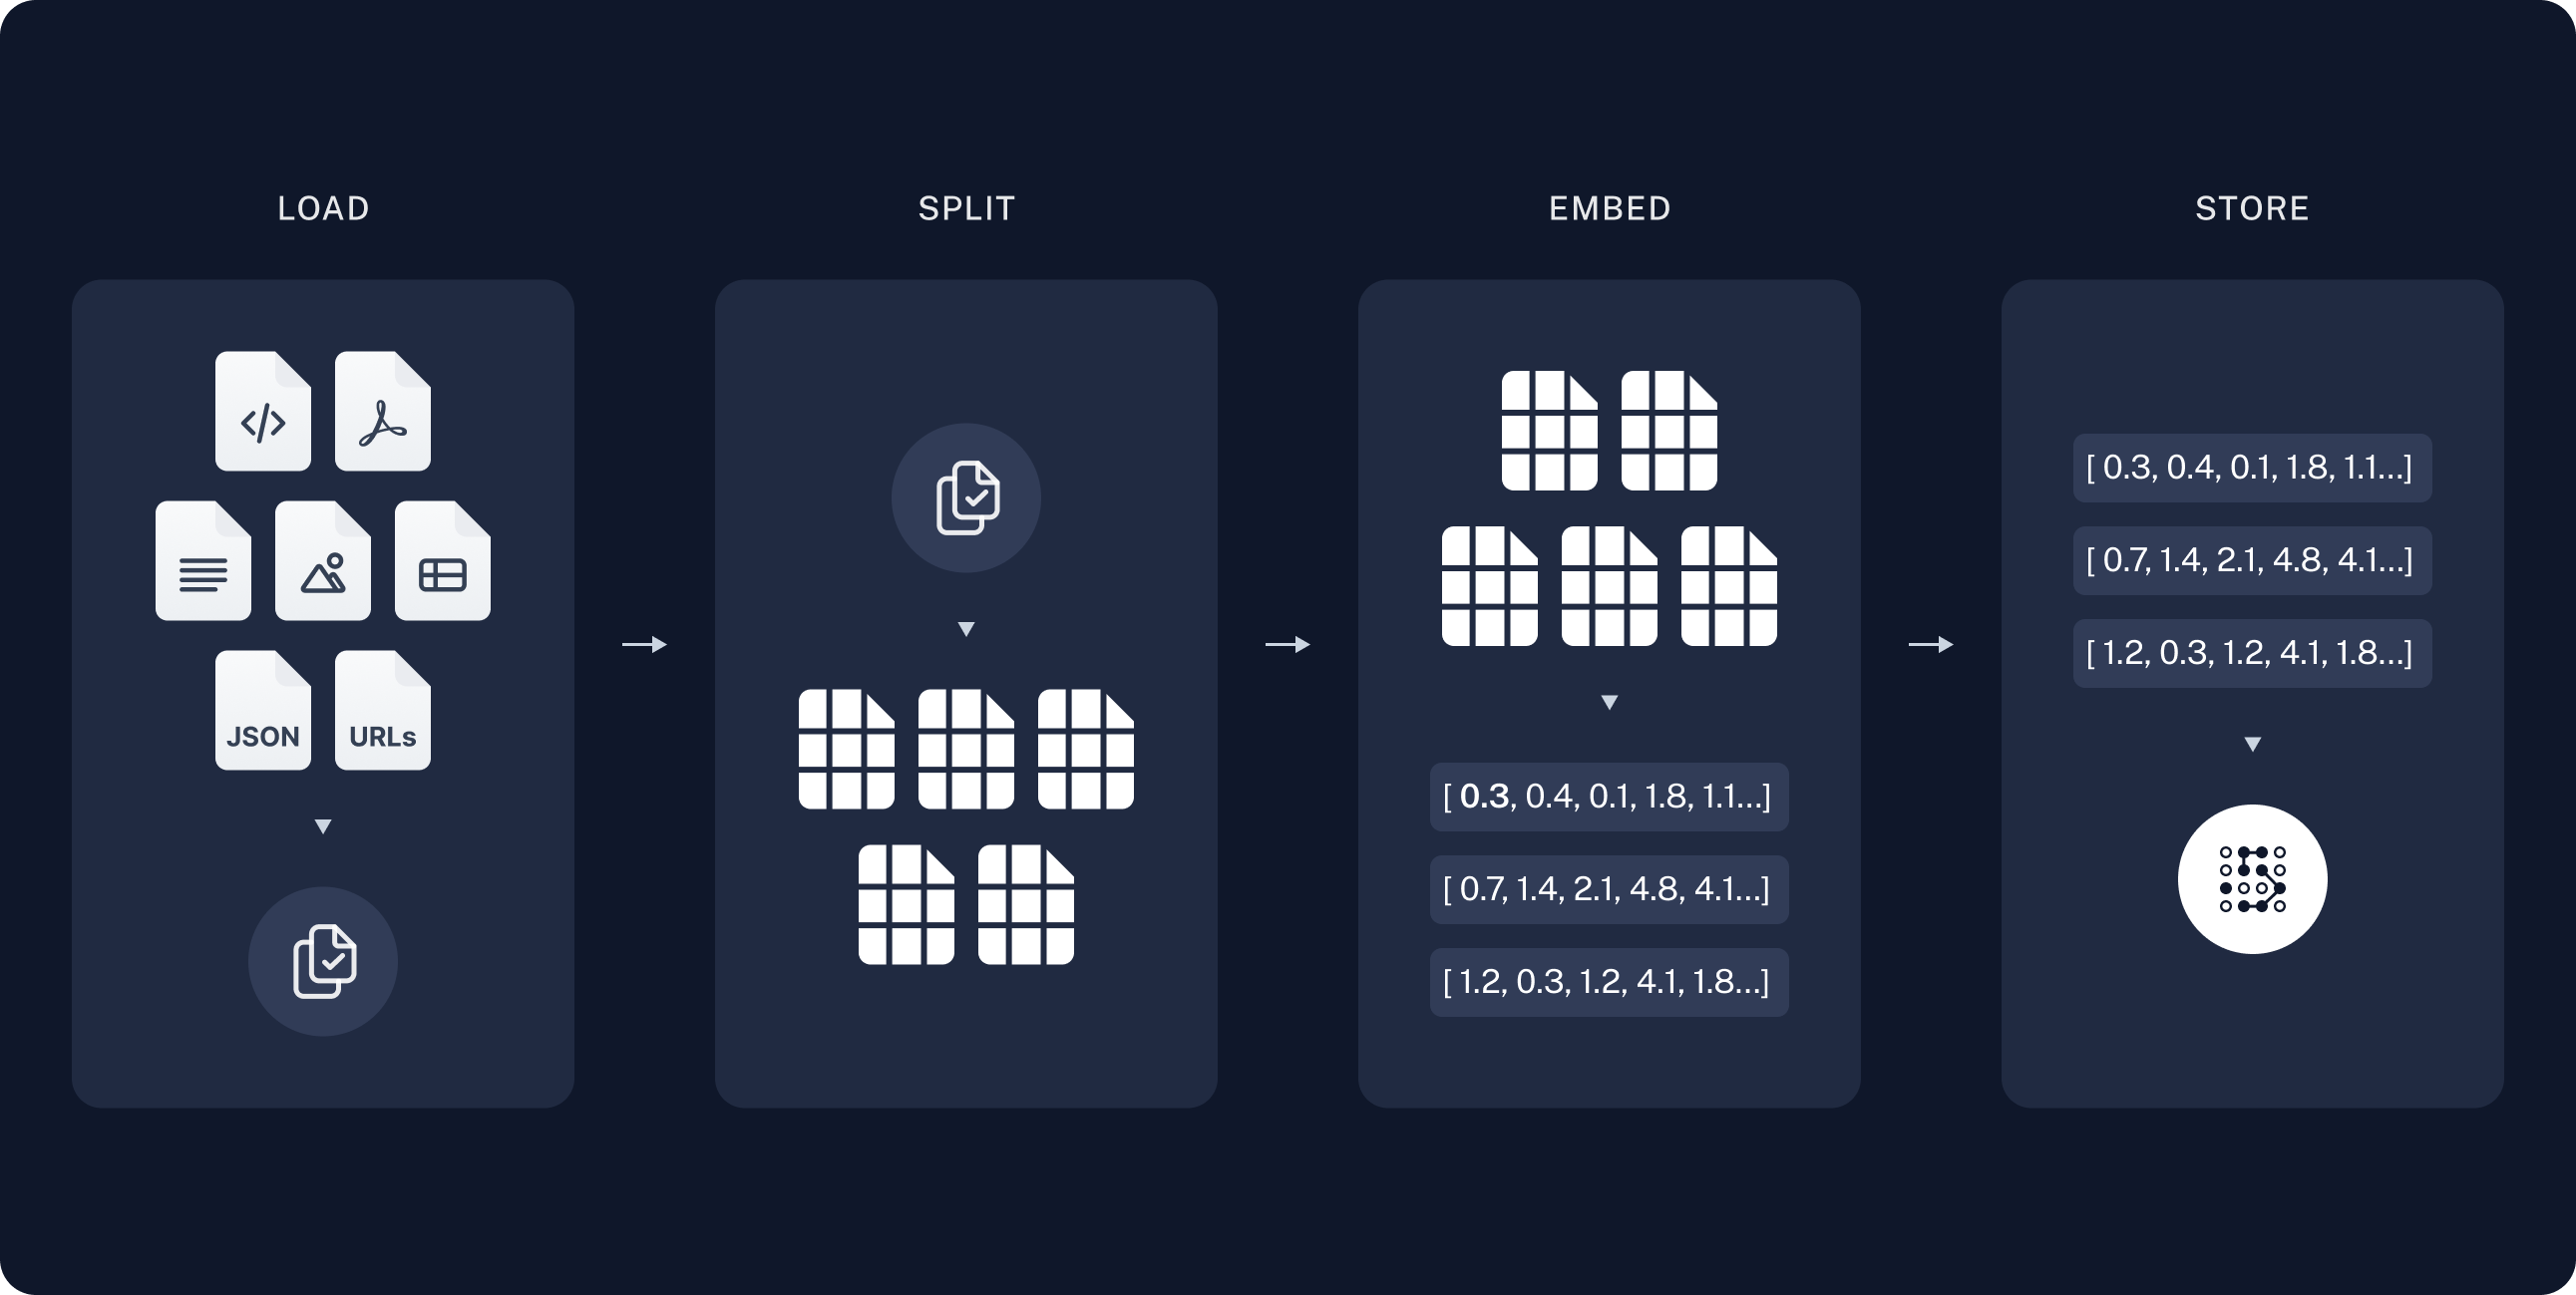
\includegraphics[width=\textwidth]{Images/cap3/rag.png}
    \caption{Indexing dei documenti in un DB Vettoriale \cite{langchainragindexing}}
    \label{fig:indexing}
\end{figure}

Per la prima prova, è stato deciso di utilizzare i documenti tratti dalla pagina Wikipedia di Keanu Reeves \cite{keanureeveswiki}.
\begin{lstlisting}[label=lst:keanusplits, caption={Preparazione degli splits dei documenti di Keanu Reeves}]
from langchain_community.document_loaders import WebBaseLoader
from langchain.text_splitter import RecursiveCharacterTextSplitter
import bs4

loader = WebBaseLoader(*@\textcolor{functionyellow}{(}@*)
    web_paths=(*@\textcolor{keywordpurple}{(}@*)(*@\textcolor{stringbrown}{"https://it.wikipedia.org/wiki/Keanu\_Reeves"}@*),(*@\textcolor{keywordpurple}{)}@*),
    bs_kwargs=(*@\textcolor{classgreen}{dict}@*)(*@\textcolor{keywordpurple}{(}@*)
        parse_only=bs4.SoupStrainer(*@\textcolor{defblue}{(}@*)
            class_=(*@\textcolor{functionyellow}{(}@*)(*@\textcolor{stringbrown}{"mw-content-ltr mw-parser-output"}@*)(*@\textcolor{functionyellow}{)}@*)
        (*@\textcolor{defblue}{)}@*)
    (*@\textcolor{keywordpurple}{)}@*),
    encoding=(*@\textcolor{stringbrown}{"utf-8"}@*)
(*@\textcolor{functionyellow}{)}@*)
splitter = RecursiveCharacterTextSplitter(*@\textcolor{functionyellow}{(}@*)
    chunk_size=(*@\textcolor{numberyellow}{350}@*),
    chunk_overlap=(*@\textcolor{numberyellow}{80}@*)
(*@\textcolor{functionyellow}{)}@*)
loaded = loader.load(*@\textcolor{functionyellow}{()}@*)
splits = splitter.split_documents(*@\textcolor{functionyellow}{(}@*)loaded(*@\textcolor{functionyellow}{)}@*)
\end{lstlisting}
Una volta ottenuti gli splits (o chunks) dei documenti, era necessario vettorizzarli prima di caricarli nel database. Grazie a LangChain queste due operazioni possono essere fatte in un solo passaggio. Per farlo è necessario disporre di due strumenti:
\begin{itemize}
    \item \textbf{Un Embedder}: Un embedder è un oggetto che prende in input un Documento e lo trasforma in un vettore numerico. Questo vettore rappresenta il contenuto del documento in uno spazio vettoriale.
    \item \textbf{Un VectorStore}: Un vectorstore è un oggetto che serve a gestire i vettori generati dagli embedders. Questi vettori vengono memorizzati nel vectorstore e possono essere recuperati in seguito tramite delle ricerche.
\end{itemize}
\begin{lstlisting}[label=lst:keanuload, caption={Caricamento degli splits sul vectorstore}]
from langchain_huggingface import HuggingFaceEmbeddings
from langchain_community.vectorstores import Chroma

model_name = (*@\textcolor{stringbrown}{"sentence-transformers/all-mpnet-base-v2"}@*)
model_kwargs = (*@\textcolor{functionyellow}{\{}@*)"device": "cuda"(*@\textcolor{functionyellow}{\}}@*)
embedder = HuggingFaceEmbeddings(*@\textcolor{functionyellow}{(}@*)
    model_name=model_name,
    model_kwargs=model_kwargs
(*@\textcolor{functionyellow}{)}@*)

vectorstore = Chroma.from_documents(*@\textcolor{functionyellow}{(}@*)
    documents=splits,
    embedding=embedder
(*@\textcolor{functionyellow}{)}@*)
\end{lstlisting}
LangChain offre la possibilità di utilizzare diversi tipi di vectorstores, e il primo che è stato provato è stato \textit{Chroma} \cite{chromadb}, che si è rivelato veloce e preciso. Lo stesso vale per l'embedder: è stato scelto il modello di default offerto da Hugging Face, vale a dire \textit{all-mpnet-base-v2} \cite{mpnet}, sebbene sarebbe stato possibile optare anche per modelli forniti da OllamaEmbeddings o altre librerie. Una volta creato il vectorstore con i vettori dei documenti, è stato possibile effettuare una ricerca all'interno del database. Per questo scopo, è stato necessario implementare un retriever, un oggetto che prende in input una query e restituisce i documenti più rilevanti rispetto alla stessa.
\begin{lstlisting}[label=lst:keanuretriever, caption={Creazione del retriever e primo retrieving}]
retriever = vectorstore.as_retriever(*@\textcolor{functionyellow}{(}@*)
    search_type="similarity", # default
    search_kwargs=(*@\textcolor{keywordpurple}{\{}@*)"k": (*@\textcolor{numberyellow}{2}@*)(*@\textcolor{keywordpurple}{\}}@*) # (*@\textcolor{commentsgreen}{default -> k=4}@*)
(*@\textcolor{functionyellow}{)}@*)
retriever.invoke(*@\textcolor{functionyellow}{(}@*)"Che film ha fatto Keanu Reeves?"(*@\textcolor{functionyellow}{)}@*)
\end{lstlisting}
Il codice in Codice \ref{lst:keanuretriever} crea un retriever e cerca i primi due documenti più simili alla query \textit{"Che film ha fatto Keanu Reeves?"}.

La ricerca dei documenti può essere fatta sia come nell'esempio, ovvero definendo un tipo di retriever a partire dal vectorstore e specificando eventualmente il tipo di ricerca (similarity, mmr, similarity\textunderscore threshold), oppure si può fare direttamente dal vectorstore utilizzando le funzioni di ricerca offerte da esso.

Una volta impostato il retriever, era possibile creare la RAG Chain:
\begin{lstlisting}[label=lst:ragchain, caption={Creazione della RAG Chain}]
from langchain_core.runnables import RunnablePassthrough
from langchain_core.output_parsers import StrOutputParser
from langchain_core.prompts import PromptTemplate

def format_docs(*@\textcolor{functionyellow}{(}@*)docs(*@\textcolor{functionyellow}{)}@*):
    return "\n\n".join(*@\textcolor{functionyellow}{(}@*)doc.page_content for doc in docs(*@\textcolor{functionyellow}{)}@*)

prompt = PromptTemplate.from_template(*@\textcolor{functionyellow}{(}@*)RAG_PROMPT(*@\textcolor{functionyellow}{)}@*)

rag_chain = (*@\textcolor{functionyellow}{(}@*)
    (*@\textcolor{keywordpurple}{\{}@*)
        "context": retriever | format_docs,
        "question": RunnablePassthrough(*@\textcolor{defblue}{()}@*)
    (*@\textcolor{keywordpurple}{\}}@*)
    | prompt
    | llm
    | StrOutputParser(*@\textcolor{keywordpurple}{()}@*)
(*@\textcolor{functionyellow}{)}@*)

rag_chain.invoke(*@\textcolor{functionyellow}{(}@*)"Che film ha fatto Keanu Reeves?"(*@\textcolor{functionyellow}{)}@*)
\end{lstlisting}
Questo basta per creare una RAG Chain che permetta di effettuare ricerche all'interno di un database di documenti e passare il risultato all'LLM per la generazione di una risposta. Da notare il prompt utilizzato, che è stato definito in precedenza nel Codice \ref{lst:prompt} e che permette di formattare l'input in modo che sia comprensibile dall'LLM. In più è stata definita una funzione \textit{format\textunderscore docs()} che permette di formattare i documenti in modo da passare solo il contenuto del documento all'LLM.

\subsection{I primi problemi}
Eseguendo lo script appena descritto, il risultato ottenuto è stato il seguente:
\begin{center}
    \textit{"Keanu Reeves è un attore che ha interpretato ruoli in diversi film, ad esempio Spalle Larghe (Youngblood) e Il fantastico mondo dei giocattoli (Babes in Toyland)."}
\end{center}
L'output è stato generato in circa 3 minuti, è corretto, ma non è dei migliori poiché avrebbe potuto includere più informazioni. Tentando nuovamente, ma senza includere il passaggio in cui il retriever cerca i documenti più simili alla query (quindi passando l'input direttamente all'LLM), l'output generato è stato il seguente:
\begin{center}
    \textit{"Keanu Reeves è un attore canadese naturalizzato statunitense. Ha recitato in molti film di successo, tra cui Speed, Matrix e John Wick."}
\end{center}
Questa volta esso è stato generato nella metà del tempo e nonostante contenga informazioni meno dettagliate, ha risposto includendo informazioni molto più varie e di maggior rilevanza. Questo output però si basa solo sulle conoscenze del modello e non su documenti caricati.

Il problema principale è che il retriever non è stato in grado di trovare i documenti più rilevanti alla query, e questo è dovuto al fatto che i documenti caricati nel database non erano sufficientemente informativi. Si è quindi deciso di testare domande più semplici, che richiedessero meno informazioni. L'input scelto è stato: \textit{"Dimmi quando e dove è nato Keanu Reeves"}, e l'output generato è stato il seguente:
\begin{center}
    \textit{"Keanu Reeves è nato nel 1964 a Beirut, in Libano, il giorno del suo compleanno."}
\end{center}
L'output generato è corretto, in quanto Keanu Reeves è effettivamente nato a Beirut, Libano, nel 1964. Tuttavia, peccava di precisione e consistenza. Si ipotizzò che il problema fosse legato al fatto che l'input ricevuto dal retriever fosse esattamente la query dell'utente, e che questo potesse non essere sufficiente per identificare i documenti più rilevanti. Inoltre, la formattazione dei dati caricati dalla pagina Wikipedia di Keanu Reeves non era ottimale, il che potrebbe aver influito sulla qualità dei risultati.

\subsection{Il DB Maker}
\label{sec:dbmaker}
Per mitigare il problema, è stata creata una struttura con il compito di gestire l'intero processo di indicizzazione dei dati grezzi. Questo sistema, evoluto nel DB Maker, prende in input una lista di oggetti di tipo \textit{Data}, ciascuno contenente tutte le informazioni necessarie per accedere ai dati che rappresentano. Tra queste informazioni, è presente un campo di tipo \textit{DataType}, che indica il tipo di dati contenuti nell'oggetto. A seconda del tipo di dato, viene utilizzato un tipo di loader differente. I dati supportati dal DB Maker sono: Web, File Testuali, Dataframe e PDF. Questi possono essere caricati singolarmente o specificando una directory, lasciando al DB Maker il compito di discernere i vari tipi di dati.

Una volta che il Maker ha ottenuto tutte le informazioni necessarie, avvia un test per verificare che i dati che si intende caricare siano esistenti e correttamente accessibili. In caso positivo, inizia il processo di caricamento e suddivisione dei dati. Una volta ottenuti gli splits, i dati vengono vettorizzati e caricati nel vectorstore. Inizialmente, è stato scelto Chroma come vectorstore, ma a causa di problemi riscontrati durante il tentativo di caricare dati di dimensioni maggiori, sono state effettuate alcune prove con altri strumenti.

È stato provato il vectorstore \textit{QDrant} \cite{qdrant}, che, nonostante la sua eccezionale velocità sia in fase di inserimento dei dati che in fase di recupero, ha mostrato imprecisione nei risultati. Il migliore, alla fine, si è rivelato essere \textit{FAISS} \cite{faiss,douze2024faisslibrary}, che si è dimostrato sia veloce che preciso.
\begin{lstlisting}[label=lst:dbmaker, caption={Implementazione del DB Maker}]
from data_manager import Data, Splitter
from langchain_community.vectorstores import FAISS
from tqdm import tqdm

class DBMaker(*@\textcolor{functionyellow}{()}@*):
    def __init__(*@\textcolor{functionyellow}{(}@*)self, config: (*@\textcolor{classgreen}{dict}@*), vectorstore: FAISS(*@\textcolor{functionyellow}{)}@*):
        self.config = config
        self.vectorstore = vectorstore
    
    def make(*@\textcolor{functionyellow}{(}@*)self, data: (*@\textcolor{classgreen}{list}@*)(*@\textcolor{keywordpurple}{[}@*)Data(*@\textcolor{keywordpurple}{]}@*)(*@\textcolor{functionyellow}{)}@*):
        splitter = Splitter(*@\textcolor{functionyellow}{(}@*)self.config(*@\textcolor{keywordpurple}{[}@*)"paths"(*@\textcolor{keywordpurple}{]}@*)(*@\textcolor{keywordpurple}{[}@*)"data"(*@\textcolor{keywordpurple}{]}@*)(*@\textcolor{functionyellow}{)}@*)
        docs = splitter.create_chunks(*@\textcolor{functionyellow}{(}@*)data(*@\textcolor{functionyellow}{)}@*)
        batches = self.batch(*@\textcolor{functionyellow}{(}@*)docs(*@\textcolor{functionyellow}{)}@*)
        for (*@\textcolor{basicblue}{batch}@*) in tqdm(*@\textcolor{functionyellow}{(}@*)
            batches,
            desc="Caricamento documenti(*@\textcolor{stringbrown}{...}@*)"
        (*@\textcolor{functionyellow}{)}@*):
            self.vectorstore.add_documents(*@\textcolor{functionyellow}{(}@*)(*@\textcolor{basicblue}{batch}@*)(*@\textcolor{functionyellow}{)}@*)
        self.vectorstore.save_local(*@\textcolor{functionyellow}{(}@*)
            self.config(*@\textcolor{keywordpurple}{[}@*)"paths"(*@\textcolor{keywordpurple}{]}@*)(*@\textcolor{keywordpurple}{[}@*)"db"(*@\textcolor{keywordpurple}{]}@*)
        (*@\textcolor{functionyellow}{)}@*)
    
    def batch(*@\textcolor{functionyellow}{(}@*)self, chunks, n_max=(*@\textcolor{numberyellow}{10000}@*)(*@\textcolor{functionyellow}{)}@*):
        batches = (*@\textcolor{functionyellow}{[]}@*)
        current_batch = (*@\textcolor{functionyellow}{[]}@*)
        count = (*@\textcolor{numberyellow}{0}@*)

        for c in chunks:
            chunk_length = len(*@\textcolor{functionyellow}{(}@*)c.page_content(*@\textcolor{functionyellow}{)}@*)
            
            if count + chunk_length >= n_max:
                batches.append(*@\textcolor{functionyellow}{(}@*)current_batch(*@\textcolor{functionyellow}{)}@*)
                current_batch = (*@\textcolor{functionyellow}{[}@*)c(*@\textcolor{functionyellow}{]}@*)
                count = chunk_length
            else:
                current_batch.append(*@\textcolor{functionyellow}{(}@*)c(*@\textcolor{functionyellow}{)}@*)
                count += chunk_length

        if current_batch:
            batches.append(*@\textcolor{functionyellow}{(}@*)current_batch(*@\textcolor{functionyellow}{)}@*)
        
        return batches
\end{lstlisting}
Il Codice \ref{lst:dbmaker} è l'implementazione del DB Maker, si noti che i documenti vengono caricati in batch di dimensioni massime di 10000 caratteri. Questo è stato fatto per evitare che la memoria di sistema si riempisse troppo velocemente.
Lo splitter invece è implementato in modo tale da prendere in input i dati grezzi e passarli al loro loader corrispondente. A quel punto effettua lo splitting dei documenti e li restituisce tutti assieme al DB Maker all'interno di una lista di oggetti di tipo Document.
\begin{lstlisting}[label=lst:loaddb, caption={Procedura di caricamento con DB Maker}]
from langchain_community.docstore import InMemoryDocstore
from langchain_community.vectorstores import FAISS
from langchain_huggingface import HuggingFaceEmbeddings

from data_manager import DataList
from (*@\textcolor{classgreen}{db\_maker}@*) import DBMaker
from utilities import load_config
from dotenv import load_dotenv, find_dotenv
import faiss
import torch
 
config = load_config(*@\textcolor{functionyellow}{()}@*)
load_dotenv(*@\textcolor{functionyellow}{(}@*)find_dotenv(*@\textcolor{keywordpurple}{()}@*)(*@\textcolor{functionyellow}{)}@*)

data_list = DataList(*@\textcolor{functionyellow}{(}@*)config(*@\textcolor{functionyellow}{)}@*)
data_list.add_dir(*@\textcolor{functionyellow}{(}@*)
    path="txts_parags/",
    chunk_size=(*@\textcolor{numberyellow}{1000}@*),
    chunk_overlap=(*@\textcolor{numberyellow}{0}@*)
(*@\textcolor{functionyellow}{)}@*)
data_list.add(*@\textcolor{functionyellow}{(}@*)path="link(*@\textcolor{stringbrown}{.}@*)txt"(*@\textcolor{functionyellow}{)}@*)

if not data_list.test(*@\textcolor{functionyellow}{()}@*):
    return
data = data_list.get_data(*@\textcolor{functionyellow}{()}@*)

model_name = config(*@\textcolor{functionyellow}{[}@*)"embedder"(*@\textcolor{functionyellow}{]}@*)
device = "cuda" if torch.cuda.is_available(*@\textcolor{functionyellow}{()}@*) else "cpu"
model_kwargs = (*@\textcolor{functionyellow}{\{}@*)"device": device(*@\textcolor{functionyellow}{\}}@*)

embedder = HuggingFaceEmbeddings(*@\textcolor{functionyellow}{(}@*)
    model_name=model_name,
    model_kwargs=model_kwargs
(*@\textcolor{functionyellow}{)}@*)

index = faiss.IndexFlatL2(*@\textcolor{functionyellow}{(}@*)
    len(*@\textcolor{keywordpurple}{(}@*)embedder.embed_query(*@\textcolor{defblue}{(}@*)"index"(*@\textcolor{defblue}{)}@*)(*@\textcolor{keywordpurple}{)}@*)
(*@\textcolor{functionyellow}{)}@*)

vectorstore = FAISS(*@\textcolor{functionyellow}{(}@*)
    embedding_function=embedder,
    index=index,
    (*@\textcolor{basicblue}{docstore}@*)=InMemoryDocstore(*@\textcolor{keywordpurple}{()}@*),
    index_to_docstore_id=(*@\textcolor{keywordpurple}{\{\}}@*)
(*@\textcolor{functionyellow}{)}@*)

db_maker = DBMaker(*@\textcolor{functionyellow}{(}@*)config, vectorstore(*@\textcolor{functionyellow}{)}@*)
db_maker.make(*@\textcolor{functionyellow}{(}@*)data(*@\textcolor{functionyellow}{)}@*)
\end{lstlisting}
In questo modo, è possibile creare un database vettoriale con i documenti di interesse e salvarlo localmente. Una volta creato il database, esso può essere utilizzato ripetutamente per eseguire ricerche nei documenti, senza la necessità di ricaricarli ogni volta.

Come illustrato all'inizio del Codice \ref{lst:loaddb}, i dati vengono caricati all'interno di un oggetto di tipo \textit{DataList}. Questi dati provengono da una directory, tranne che per un singolo file contenente alcuni link, che viene caricato singolarmente. Dopo che i dati sono stati inseriti, vengono sottoposti a un test per verificare che siano corretti e accessibili. Se il test ha esito positivo, i dati possono essere caricati nel vectorstore.

Per l'embedder, viene utilizzato lo stesso modello degli esempi precedenti (vedi Codice \ref{lst:keanuload}). Per quanto riguarda il vectorstore, si utilizza FAISS, che richiede (oltre ai documenti e all'embedder) un indice e un docstore. L'indice è un oggetto di tipo \textit{faiss.IndexFlatL2}, un indice piatto con distanza euclidea che si occupa di memorizzare i vettori veri e propri e gestire la loro ricerca. Il docstore è un oggetto di tipo \textit{InMemoryDocstore}, che serve a memorizzare i dati dei documenti in memoria. Quando viene trovato un determinato vettore, è possibile accedere al suo ID e, di conseguenza, al documento corrispondente nel docstore  (tramite l'indice \textit{index\textunderscore to\textunderscore docstore\textunderscore id}). In questo modo, è possibile recuperare i dati del documento associato al vettore trovato.

\chapter{OmniBot: L'evoluzione}
I primi esperimenti condotti non hanno dato risultati soddisfacenti, ma hanno permesso di individuare i punti deboli del sistema e di capire come migliorarlo. In questo capitolo verrà descritta l'evoluzione del progetto, partendo dal primo prototipo fino ad arrivare alla versione finale di OmniBot.

\section{Il primo prototipo}
Fino a questo punto dello sviluppo, il sistema era composto da una sola implementazione elementare di RAG, purtroppo questa versione non era in grado di gestire conversazioni complesse e non era in grado di fornire risposte di qualità accettabili. Per questo motivo, si è deciso di rivedere l'intera architettura del sistema e di introdurre nuove funzionalità.

\subsection{History Aware Retriever}
Un punto critico del sistema era il retriever, che non era in grado di recuperare i documenti migliori durante le conversazioni complesse. Questo perché il retriever non teneva conto della cronologia dei messaggi scambiati durante la conversazione. Per risolvere questo problema, ne è stato implementato uno nuovo, chiamato History Aware Retriever (HAR).

\subsubsection{La Query Transformation}
Il funzionamento dell'HAR è abbastanza semplice: durante una conversazione, esso tiene traccia di tutti i messaggi scambiati e quando un utente invia una query, anziché usare la query stessa per recuperare i documenti, la trasforma in una nuova query che tiene conto della cronologia dei messaggi scambiati \cite{fu2023complexitybasedpromptingmultistepreasoning}. In questo modo, l'HAR è in grado di recuperare i documenti più rilevanti per la conversazione in corso.
Il problema principale è stato capire come trasformare la query in modo tale che essa potesse effettivamente aiutare il retriever a recuperare documenti di qualità superiore.

\subsubsection{Implementazione e Test dell'HAR}
LangChain mette a disposizione una struttura omonima capace di gestire la cronologia dei messaggi. Per implementare l'HAR è stato sufficiente utilizzare questi strumenti e integrarli con il retriever esistente:
\begin{lstlisting}[label=lst:har, caption={Implementazione dell'History Aware Retriever}]
from langchain.chains.history_aware_retriever import create_history_aware_retriever
from langchain.chains.retrieval import create_retrieval_chain
from langchain.chains.combine_documents import create_stuff_documents_chain
from langchain_core.runnables.history import RunnableWithMessageHistory
from langchain_core.prompts import ChatPromptTemplate, MessagesPlaceholder
from langchain_ollama.llms import OllamaLLM

transform_prompt = ChatPromptTemplate.from_messages(*@\textcolor{functionyellow}{(}@*)
    (*@\textcolor{keywordpurple}{[}@*)
        (*@\textcolor{defblue}{(}@*)"system", TRANSFORM_PROMPT(*@\textcolor{defblue}{)}@*),
        MessagesPlaceholder(*@\textcolor{defblue}{(}@*)"chat_history"(*@\textcolor{defblue}{)}@*),
        (*@\textcolor{defblue}{(}@*)"human", "(*@\textcolor{defblue}{\{user\_input\}}@*)"(*@\textcolor{defblue}{)}@*),
    (*@\textcolor{keywordpurple}{]}@*)
(*@\textcolor{functionyellow}{)}@*)

llm = OllamaLLM(*@\textcolor{functionyellow}{(}@*)
    model="llama3",
    base_url=(*@\textcolor{stringbrown}{"http://localhost:11434"}@*),
    temperature=(*@\textcolor{numberyellow}{0}@*)
(*@\textcolor{functionyellow}{)}@*)

retriever = create_history_aware_retriever(*@\textcolor{functionyellow}{(}@*)
    llm, retriever, transform_prompt
(*@\textcolor{functionyellow}{)}@*)

rag_prompt = ChatPromptTemplate.from_messages(*@\textcolor{functionyellow}{(}@*)
    (*@\textcolor{keywordpurple}{[}@*)
        (*@\textcolor{defblue}{(}@*)"system", RAG_PROMPT(*@\textcolor{defblue}{)}@*),
        MessagesPlaceholder(*@\textcolor{defblue}{(}@*)"chat_history"(*@\textcolor{defblue}{)}@*),
        (*@\textcolor{defblue}{(}@*)"human", "(*@\textcolor{defblue}{\{user\_input\}}@*)"(*@\textcolor{defblue}{)}@*),
    (*@\textcolor{keywordpurple}{]}@*)
(*@\textcolor{functionyellow}{)}@*)

qa_chain = create_stuff_documents_chain(*@\textcolor{functionyellow}{(}@*)llm, rag_prompt(*@\textcolor{functionyellow}{)}@*)
rag_chain = create_retrieval_chain(*@\textcolor{functionyellow}{(}@*)retriever, qa_chain(*@\textcolor{functionyellow}{)}@*)

chain = RunnableWithMessageHistory(*@\textcolor{functionyellow}{(}@*)
    rag_chain,
    get_chat_history,
    input_messages_key="user_input",
    history_messages_key="chat_history",
    output_messages_key="answer"
(*@\textcolor{functionyellow}{)}@*)
\end{lstlisting}
Questo codice sfrutta due diversi prompt, uno è il RAG\_PROMPT (vedi Codice \ref{lst:prompt}) che viene utilizzato per passare i documenti, l'altro è il TRANSFORM\_PROMPT che viene utilizzato per trasformare la query in base alla cronologia dei messaggi. Quest'ultimo prompt può essere definito come segue:
\begin{lstlisting}[label=lst:trprompt, caption={Definizione del TRANSFORM\_PROMPT}, literate={.}{{\textcolor{stringbrown}{.}}}1 {,}{{\textcolor{stringbrown}{,}}}1 {=}{{\textcolor{white}{=}}}1]
TRANSFORM_PROMPT = (*@\textcolor{stringbrown}{"""Riformula la query in base alla seguente}@*)
                      (*@\textcolor{stringbrown}{cronologia di messaggi:}@*)
                      (*@\textcolor{defblue}{\{chat\_history\}}@*)
                
                      (*@\textcolor{stringbrown}{NON rispondere alla domanda,}@*)
                      (*@\textcolor{stringbrown}{ma riformulala in modo che}@*)
                      (*@\textcolor{stringbrown}{possa essere compresa anche}@*)
                      (*@\textcolor{stringbrown}{senza aver accesso ai precedenti}@*)
                      (*@\textcolor{stringbrown}{messaggi.}@*)
                      (*@\textcolor{stringbrown}{QUERY:}@*)
                      (*@\textcolor{defblue}{\{user\_input\}}@*)(*@\textcolor{stringbrown}{"""}@*)
\end{lstlisting}
In questo modo il modello non dovrebbe rispondere alla domanda passata, ma dovrebbe trasformare quella attuale in una migliore per il retriever. Ad esempio, se l'utente ha parlato fino ad un certo punto di "gatti" e ad un certo punto dovesse chiedere \textit{"Che cosa mangiano?"}, l'LLM dovrebbe trasformare la query in \textit{"Cosa mangiano i gatti?"}. Naturalmente questa procedura rallenta il sistema, poiché per ogni query esso deve eseguire due richieste. Infatti, non è stato raro che il sistema impiegasse più di 5 minuti per iniziare a rispondere ad una query (questo però accadeva solo dal secondo messaggio in poi, poiché il primo non richiedeva alcuna trasformazione). In più, spesso la fase di trasformazione non funzionava correttamente, restituendo query che non avevano senso o che non erano correlate alla conversazione in corso. L'unica parte davvero funzionante era il RunnableWithMessageHistory, che permetteva di tenere traccia della cronologia dei messaggi salvandoli all'interno di un dizionario ogni volta che veniva scambiato un messaggio.

\subsection{Streamlit}
\begin{figure}[!t]
    \centering
    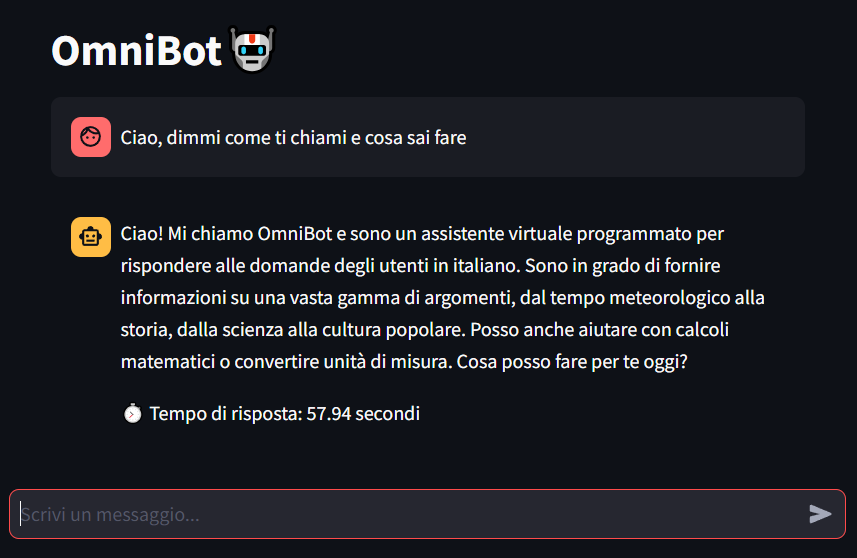
\includegraphics[width=\textwidth]{Images/cap4/streamlit.PNG}
    \caption{Interfaccia utente di OmniBot realizzata con Streamlit}
    \label{fig:streamlit}
\end{figure}
Si è ipotizzato che la causa principale degli esperimenti falliti della Query Transformation fosse il modello di linguaggio utilizzato. Nonostante ciò, si è deciso inizialmente di rimandare la sostituzione dell'LLM e di concentrarsi su un'altra parte del progetto: l'interfaccia utente. Per fare ciò è stato utilizzato Streamlit \cite{streamlit}, un framework per la creazione di applicazioni web in Python. Esso è molto semplice da utilizzare e permette di creare applicazioni web interattive in pochissimo tempo. In più, è molto flessibile e permette di integrare facilmente modelli di machine learning all'interno delle applicazioni web. L'interfaccia utente permette di inviare messaggi al sistema e di visualizzare le risposte generate dallo stesso (vedi \figurename{~\ref{fig:streamlit}}).

\section{La prima Chain-of-Thoughts}
Dopo aver compreso che l'HAR rappresentava una soluzione interessante, ma che il modello disponibile non risultava ottimale, è stata sviluppata una struttura più complessa, ossia una catena di pensiero finalizzata a facilitare il dialogo tra l'LLM e l'utente. Per raggiungere tale obiettivo, sono stati nuovamente impiegati gli strumenti messi a disposizione da LangChain, portando così alla creazione della prima Chain-of-Thoughts (CoT).
\begin{figure}[!t]
    \centering
    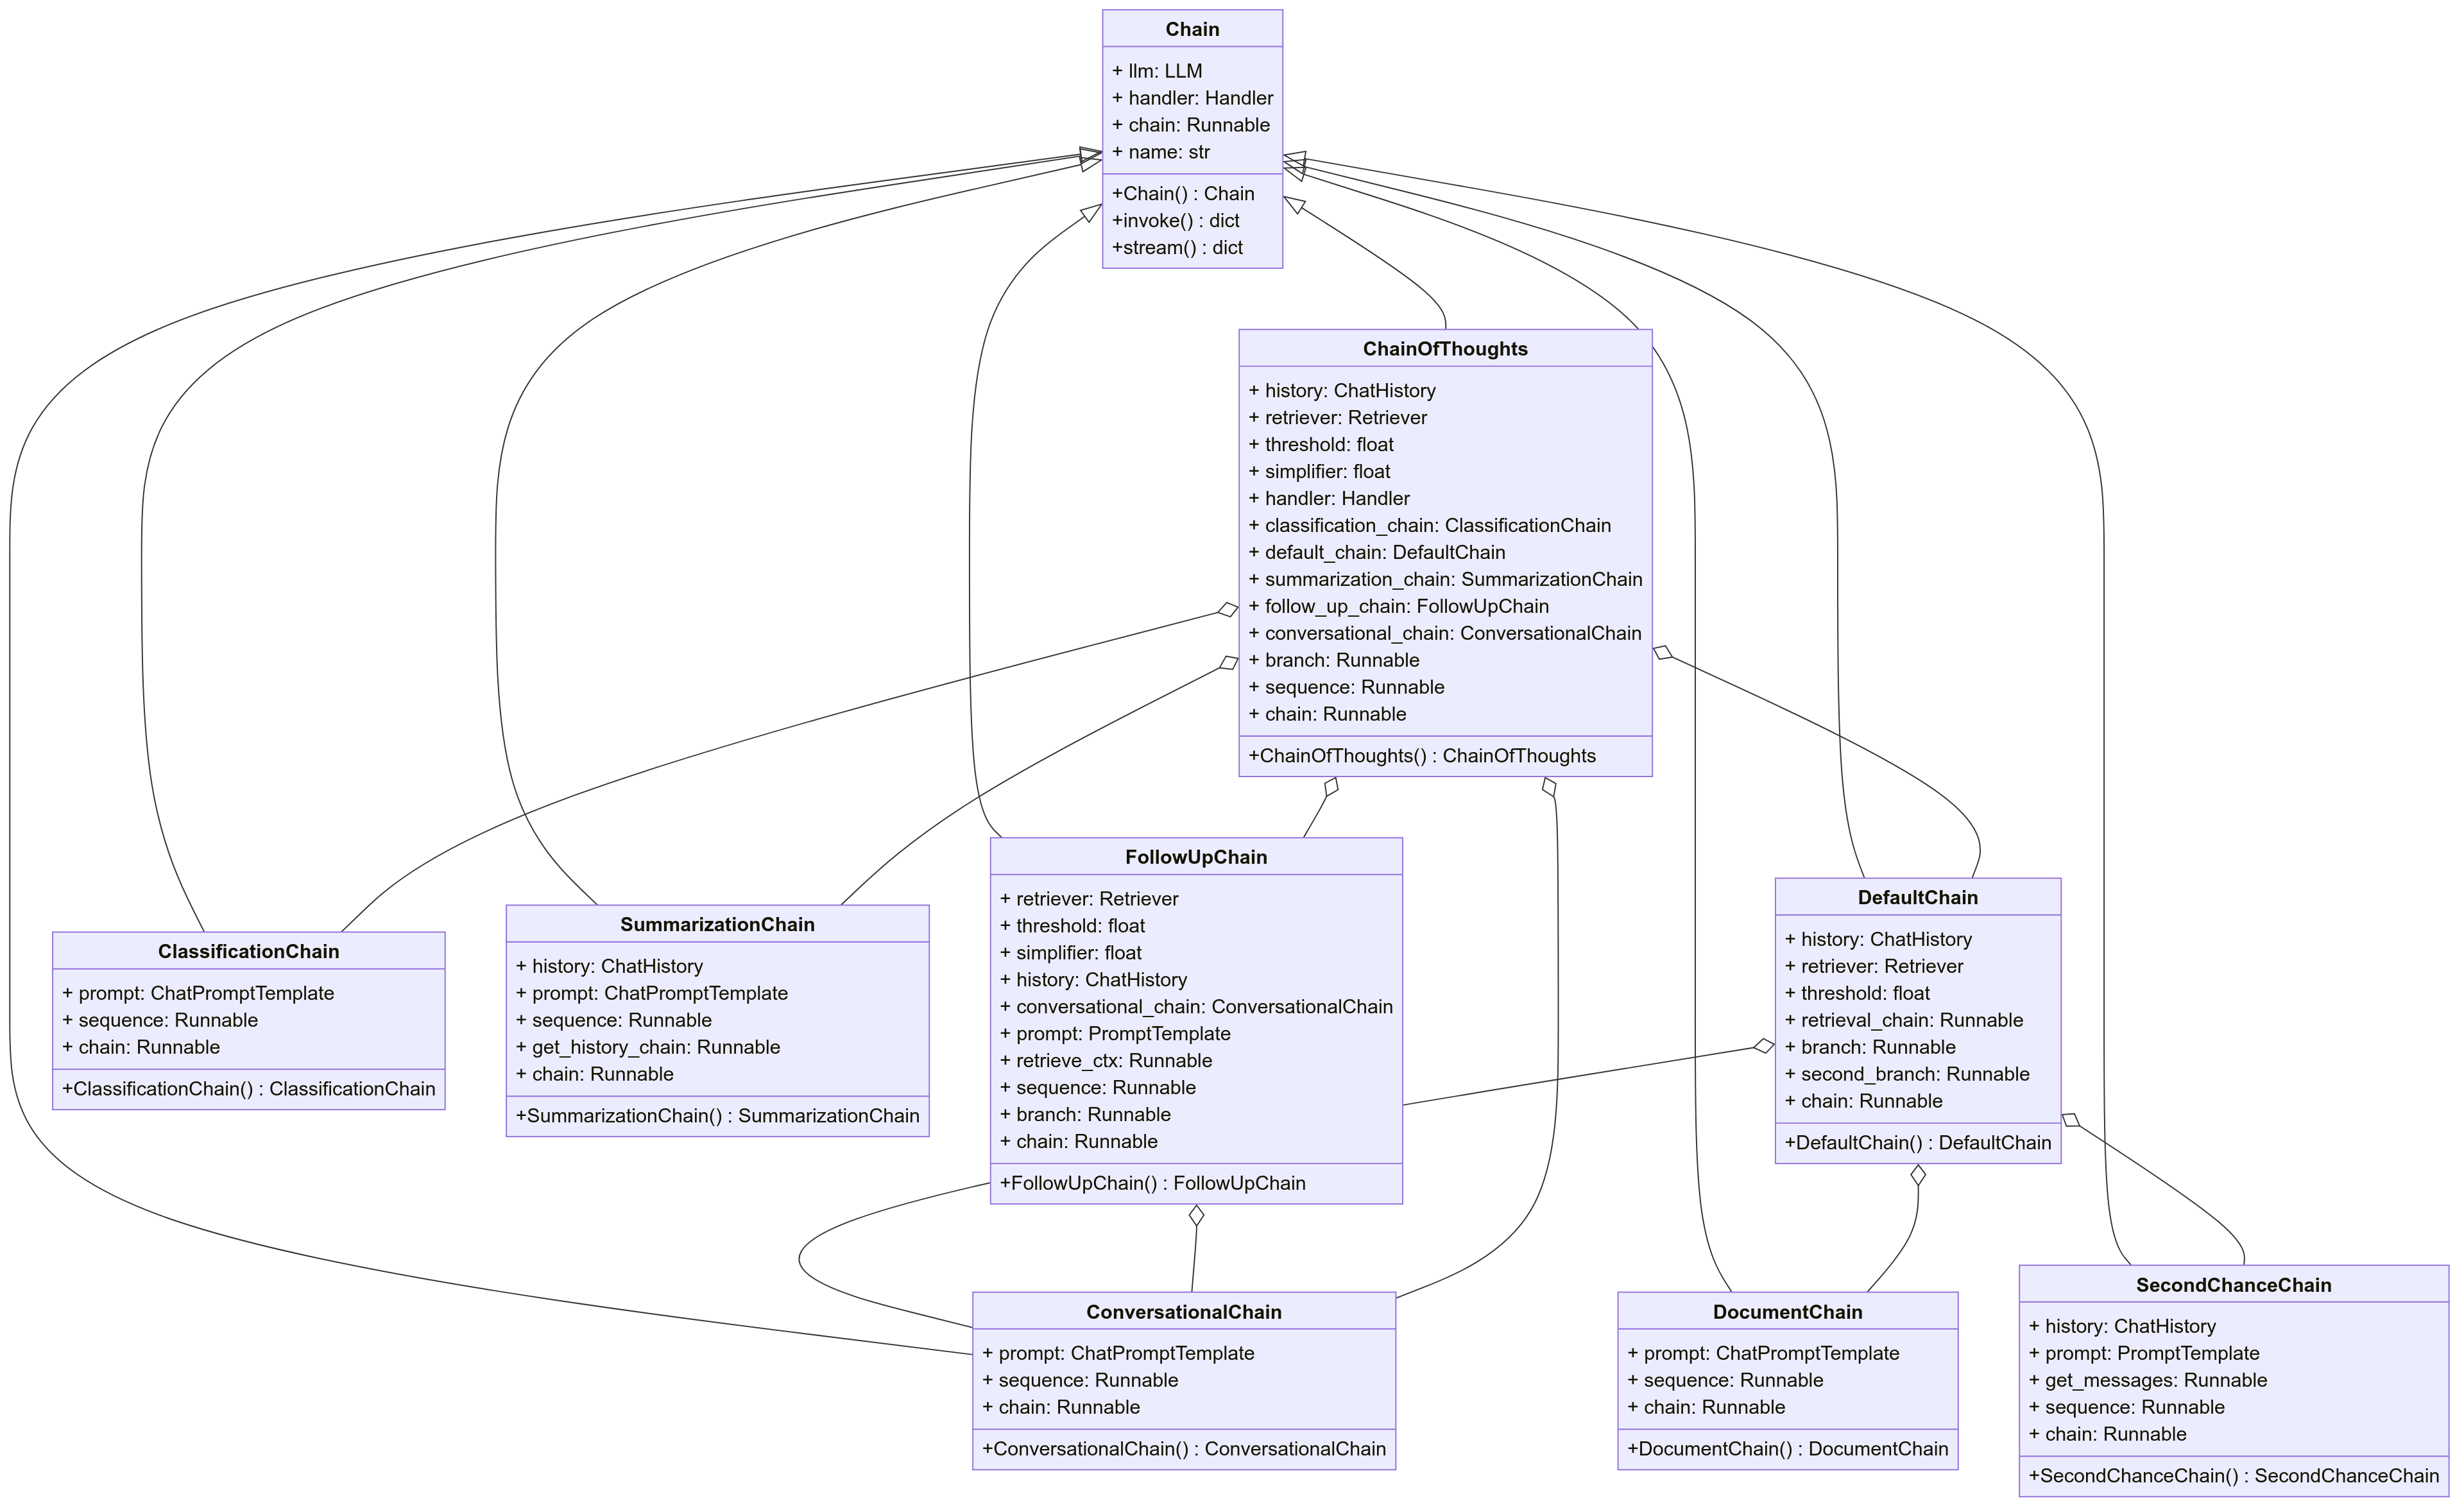
\includegraphics[width=\textwidth]{Images/cap4/schema1.png}
    \caption{Diagramma UML della prima Chain-of-Thoughts}
    \label{fig:uml1}
\end{figure}
Secondo l'idea alla base del modello, questo avrebbe dovuto riflettere su quanto comunicato dall'utente e rispondere in modo coerente. In particolare, si è ritenuto essenziale come primo passo comprendere pienamente la richiesta dell'utente per poi fornire una risposta adeguata.

\subsection{Classification Chain}
La prima parte dell'elaborazione della catena inizia con un rapido controllo sulla dimensione della ChatHistory, se questa è vuota, la catena principale avvierà la Default Chain (vedi Paragrafo \ref{sec:defaultchain}), altrimenti la Classification Chain. Questa catena ha il compito di capire che tipo di domanda ha posto l'utente.
Questa classificazione avviene passando la query al modello all'interno di un prompt specializzato. La catena darà in output un dizionario contenente la classificazione della domanda. Le classificazioni possibili sono: "conversational", "document", "summary" e "followup". Queste classificazioni sono state scelte in base alle possibili risposte che il generatore può dare. Se la classificazione non è chiara, la catena restituirà "default".

Questa catena ha avuto un discreto successo, riuscendo a classificare correttamente la maggior parte delle domande. Tuttavia, grazie all'introduzione di una nuova versione del modello in uso, la classificazione è diventata molto più precisa e affidabile. Il nuovo LLM utilizzato è Llama3.1-8B \cite{llama318b}.

\subsection{Default Chain}
\label{sec:defaultchain}
Questa è la catena responsabile della maggior parte delle interazioni con l'utente. Quando si avvia effettua una chiamata al retriever ed esso restituirà i documenti più simili alla query. Questi vengono poi filtrati in base alla loro similarità secondo un certo threshold. Se non ci sono documenti, allora passa il controllo ad una catena di \textit{fallback} chiamata Second Chance Chain. Se invece ci sono documenti, la catena passa il controllo alla Document Chain.

\subsubsection{Document Chain}
La Document Chain è la catena responsabile di gestire le domande che richiedono una risposta basata su documenti. Essa non effettua una chiamata al retriever poiché i documenti sono già stati recuperati dalla Default Chain.

\subsubsection{Second Chance Chain}
La Second Chance Chain è una catena di fallback che viene attivata quando il retriever non è in grado di recuperare documenti al primo passaggio nella Default Chain. Essa effettua una nuova chiamata al retriever, ma questa volta con una query differente. La query è generata a partire dalla query originale sfruttando la stessa tecnica utilizzata per sviluppare l'History Aware Retriever. In questo caso però sopraggiunge il \textit{simplifier}, vale a dire un numero compreso tra 0 e 1 che, moltiplicato per il threshold inziale, lo diminuisce rendendo il filtro meno restrittivo. Se anche questa catena non è in grado di recuperare documenti, allora si passa il controllo alla Conversational Chain.

\subsubsection{Conversational Chain}
La Conversational Chain è la catena responsabile di gestire le domande che richiedono una risposta conversazionale ed eventualmente le richieste che non sono state gestite dalle altre catene. Spesso e volentieri tratta richieste che non hanno a che fare con i compiti prestabiliti del chatbot. Questa catena è in grado di generare risposte in modo autonomo, senza bisogno di documenti o di una conversazione pregressa.

\subsection{Summarization Chain}
Essa è responsabile di generare un riassunto della conversazione in corso. Si tratta dell'unica che ha accesso diretto alla ChatHistory ai fini di prendere le informazioni dei messaggi scambiati e generare nuovi messaggi a partire da essi. Ad esempio, la Second Chance Chain usa la ChatHistory per generare una nuova query, ma non passa questa al modello durante la generazione dell'output finale.

\subsection{Follow-up Chain}
Di estrema importanza è anche la catena di followup, che si occupa di rispondere a domande che richiedono di approfondire un argomento già trattato. Le domande di followup possono essere di due tipi: può trattarsi di domande dirette, che esplicitano l'argomento che si vuole approfondire, ad esempio, tornando alla chat sui gatti \textit{"Conosci altri animali domestici?"}, oppure di domande che non esplicitano l'argomento, ma che si riferiscono probabilmente a qualcosa appena detta.
La catena di followup si occupa anche di capire come procedere al recupero dei documenti corretti. Per fare ciò utilizza la ChatHistory, ma non va ad analizzare solo il contenuto dei messaggi precedenti, ma anche i documenti che sono stati recuperati per rispondere a tali domande poste in precedenza. Ogni istanza di ogni messaggio conserva pure i documenti usati per ottenere la risposta. Per capire quali usare, la catena avvia una chiamata all'embedder con tutti i dati dei messaggi da confrontare e, tramite l'utilizzo di una tecnica di clustering chiamata \textit{TF-IDF} \cite{li2024documenttypeclassificationusing}, riesce a capire quali documenti sono più simili tra loro e quindi quali sono i documenti più rilevanti per la domanda posta. Questa procedura viene effettuata prima sui soli dati dell'ultimo messaggio, ma nel caso in cui non abbia successo, viene effettuata anche su tutti gli altri. Questi documenti vengono poi passati al modello per ottenere l'output.

\subsection{I punti critici di CoT}
La prima versione della Chain-of-Thoughts ha dato grandi soddisfazioni, riuscendo a portare avanti discussioni in maniera fluida e coerente alle richieste dell'utente. Tuttavia, sono emersi anche numerosi punti critici che spesso hanno portato a generare conversazioni ripetitive e concettualmente errate. I principali problemi riscontrati sono:
\begin{itemize}
    \item \textbf{Poca flessibilità}: Al modello era richiesto di parlare solo di alcuni argomenti specifici, e questi corrispondevano a quelli trattati nei documenti. Gli argomenti trattati erano spesso variegati e ciò lo portava a rifiutarsi di parlare di argomenti diversi dal primo argomento trattato durante la conversazione.
    \item \textbf{Limiti non rispettati}: Le stesse indicazioni che impedivano ad esso di sproloquiare o di parlare di argomenti non di sua pertinenza, a volte venivano ignorate.
    \item \textbf{Approfondimenti insoddisfacenti}: Spesso il sistema di recupero dei documenti provenienti dallo store dei documenti di chat non andava a buon fine e questo portava l'LLM a inventare informazioni o nuovamente a rifiutarsi di parlare oltre.
    \item \textbf{Retrieving non pertinente}: Il retriever non era sempre in grado di restituire i documenti migliori o addirittura non restituiva documenti. Questo per via del threshold statico che non dava un largo margine al filtro. Abbassando il threshold, d'altra parte, il rischio era di ricevere documenti con bassa rilevanza.
    \item \textbf{Punteggi di similarità errati}: I punteggi di similarità associati ai documenti restituiti dal retriever non erano sempre corretti. Capitava di avere documenti ottimi con valori di similarità bassi e viceversa.
    \item \textbf{Problemi di memoria}: Il modello faticava nel rispondere a domande che facevano riferimento a messaggi precedenti, poiché questi non gli venivano mai passati direttamente nel contesto se non con la Summarization Chain.
    \item \textbf{Errori di classificazione}: La Classification Chain era fondamentale per capire che tipo di domanda l'utente aveva posto, ma in molte occasioni capitava che non riuscisse a classificare correttamente le domande portando il modello a rispondere in maniera errata.
    \item \textbf{Tempi di risposta lunghi}: Il sistema era molto complesso e richiedeva di effettuare 2 o addirittura 3 chiamate al LLM per rispondere a una singola domanda. Questo portava a tempi di risposta molto lunghi, spesso superiori ai 10 minuti.
\end{itemize}

\section{La Chain-of-Thoughts ridefinita}
Dopo aver individuato i punti critici della prima versione della Chain-of-Thoughts, l'intera architettura del sistema è stata riprogettata, apportando diverse modifiche significative.
\begin{figure}[!t]
    \centering
    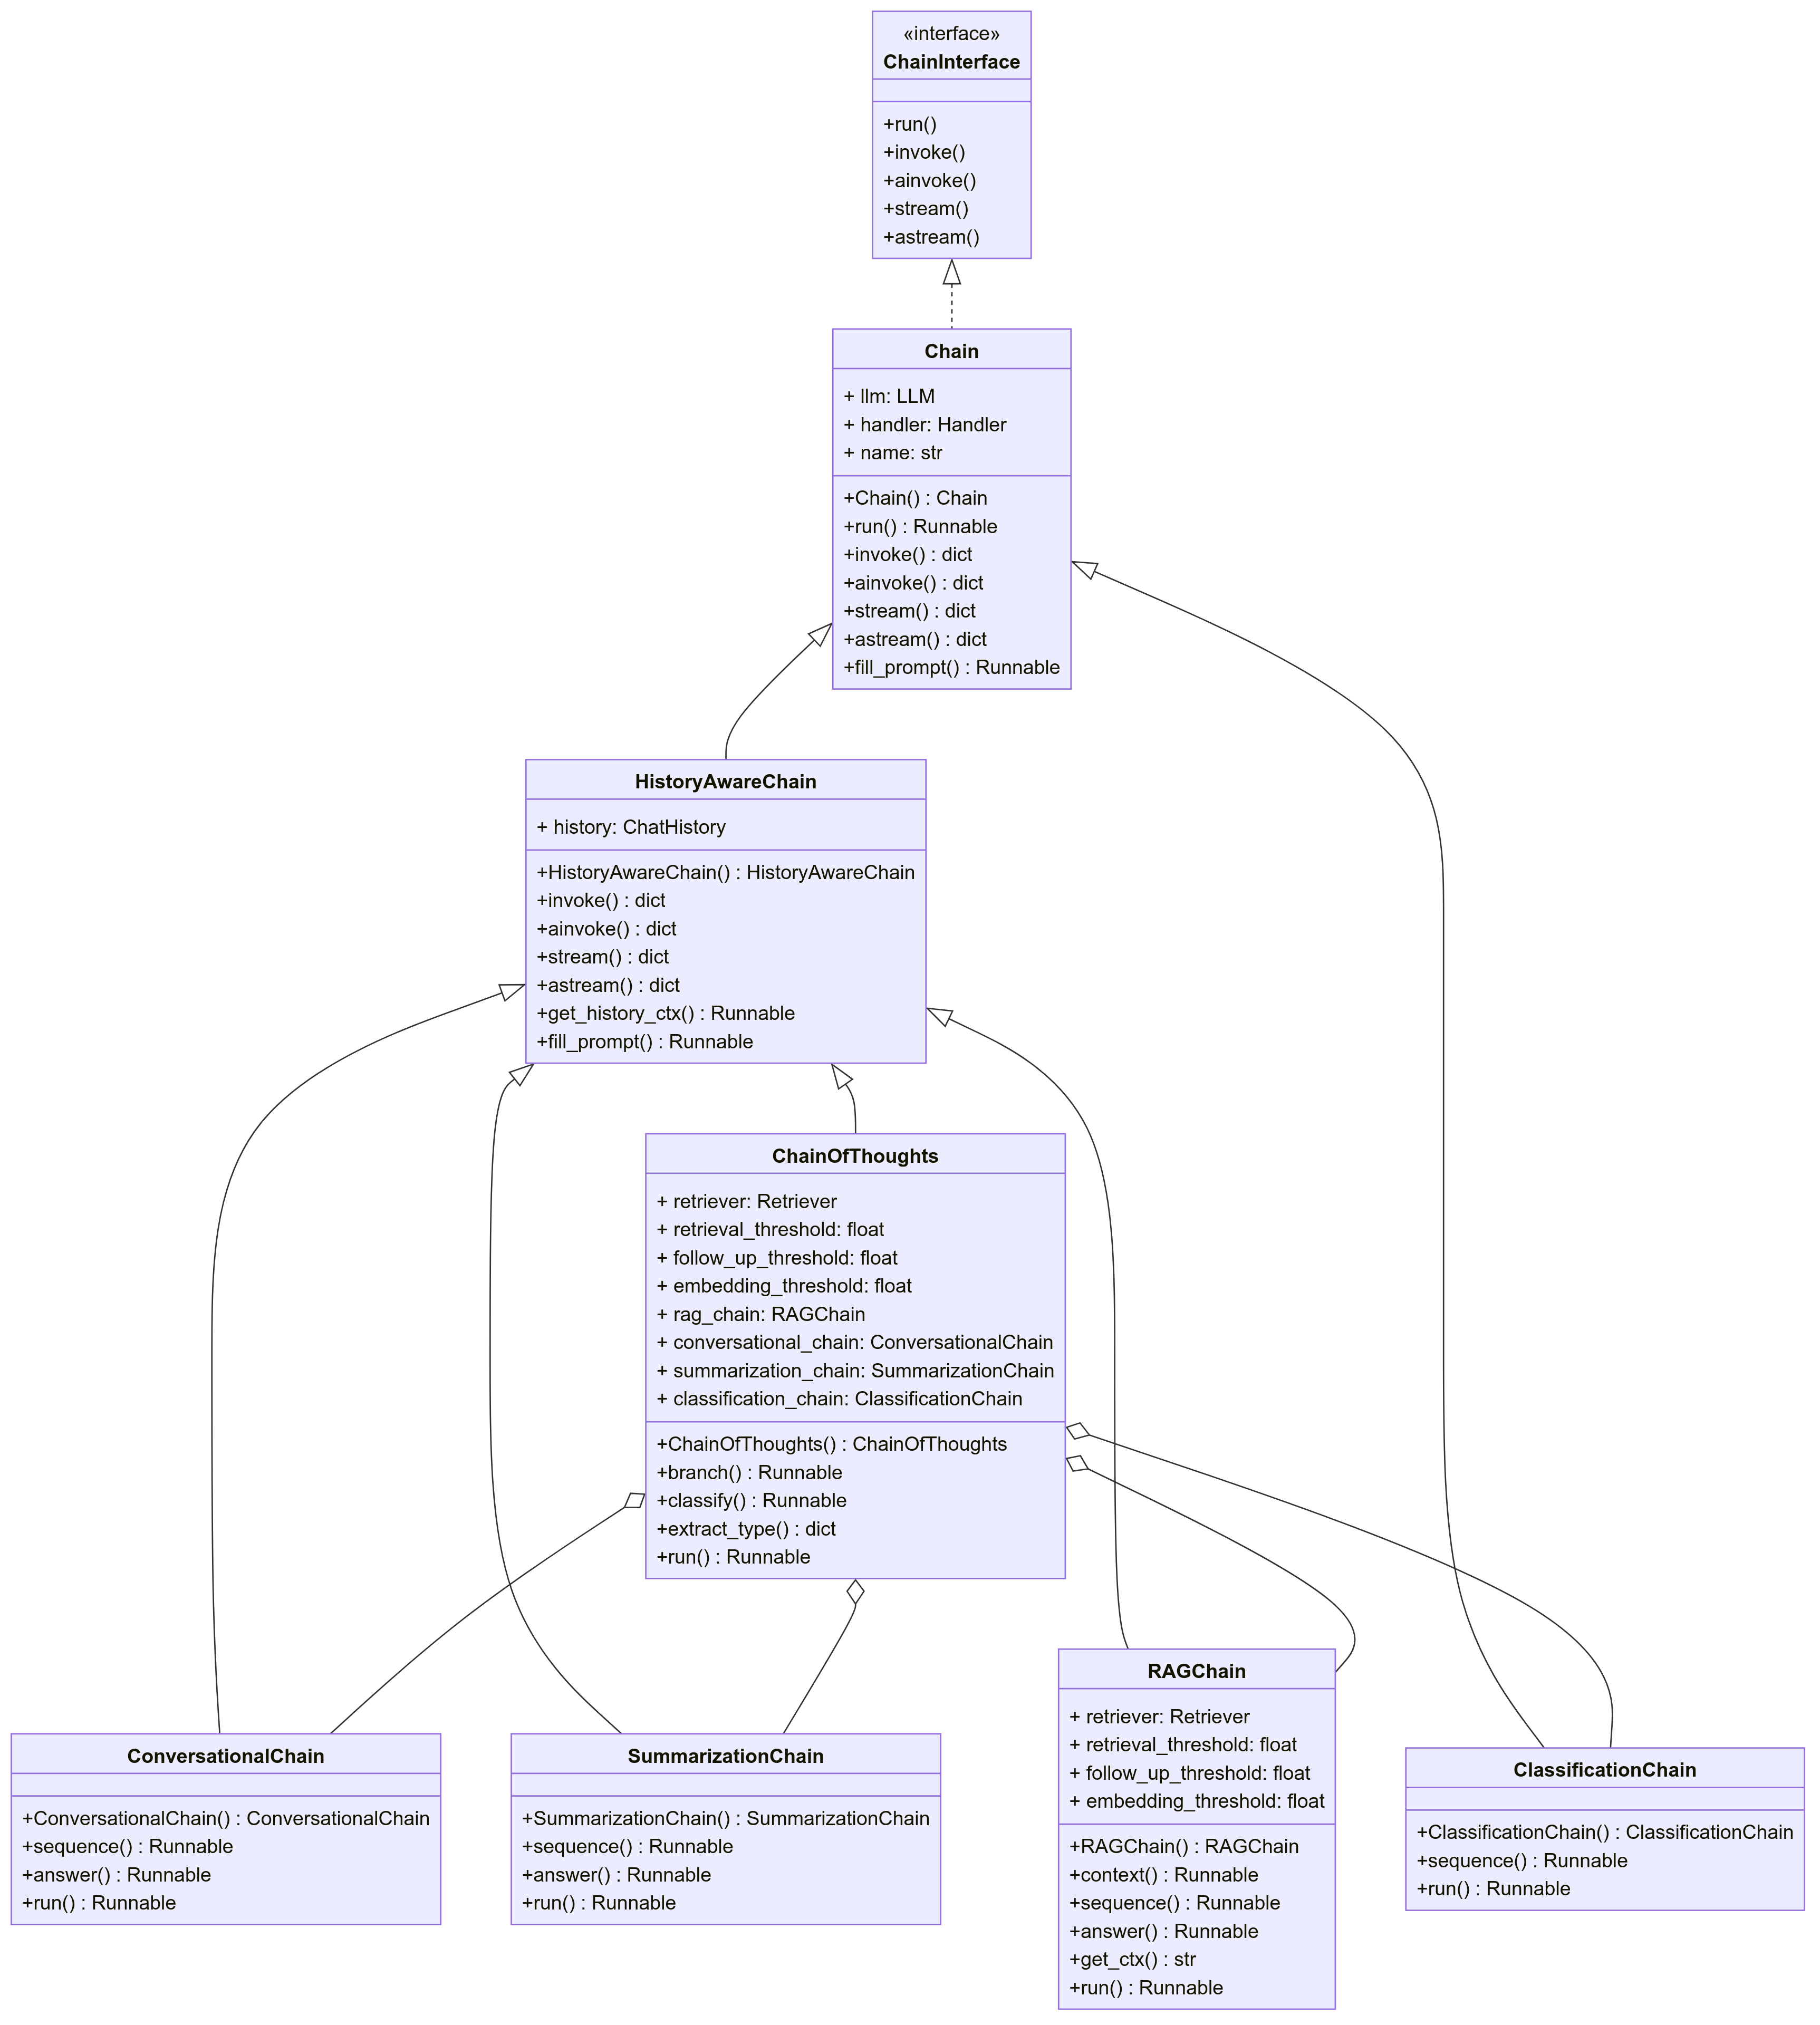
\includegraphics[width=\textwidth]{Images/cap4/schema2.png}
    \caption{Diagramma UML della nuova Chain-of-Thoughts}
    \label{fig:uml2}
\end{figure}
Il metodo più efficace è stato il refactoring della CoT e dei suoi sottosistemi. In questo processo, si è potuto usufruire anche di nuove risorse hardware fornite dall'azienda di tirocinio \cite{intellisync}: un computer dotato di 32 GB di RAM, un processore Intel Core i7 di 10ª generazione e una GPU NVIDIA GeForce RTX 3070 Ti da 8 GB. Grazie a questa configurazione più potente, è stata ottenuta l'opportunità di testare modelli più grandi e performanti.

\subsubsection{Mistral-Nemo e Dolphin}
Il primo modello testato è stato Mistral-Nemo \cite{mistralnemo12b}, che possedeva circa 12B di parametri. Sviluppato da Mistral AI in collaborazione con NVIDIA era capace di gestire un contesto massimo di 128k token. Quantizzato in formato Q4, questo modello pesa solo 7,1 GB, permettendo il caricamento completo sulla VRAM. Le prestazioni di Mistral-Nemo si sono dimostrate nettamente superiori rispetto a Llama3.1-8B, specialmente nella fase di classificazione, risolvendo quasi del tutto i problemi iniziali legati alla Classification Chain. Inoltre, anche i problemi relativi al mancato rispetto delle limitazioni o all'eccessiva fissazione sul primo argomento discusso sembravano essere stati risolti. Grazie alla nuova scheda grafica, i tempi di risposta si sono ridotti drasticamente, passando da circa 5 minuti a soli 30 secondi per domanda. La reattività del sistema è stata ulteriormente migliorata con il supporto per lo streaming dei token in output, permettendo di ricevere risposte parziali già dopo pochi istanti.

Nonostante questi significativi miglioramenti, sono state esplorate anche altre opzioni su Hugging Face, dove è stata trovata una versione non censurata di Mistral-Nemo, il modello Dolphin 2.9.3 Mistral-Nemo 12B \cite{dolphin}. Questo, caricato tramite Ollama, è più veloce e leggero rispetto alla versione censurata. Si è optato per la versione con quantizzazione Q4KM, con un peso di 7,48 GB. Sebbene fosse leggermente più grande della VRAM disponibile, impedendo il suo completo caricamento sulla GPU, non ha comportato rallentamenti significativi. In alcuni casi, Dolphin si è persino dimostrato più veloce di Mistral-Nemo.

\subsection{History Aware Chain}
Per risolvere i problemi legati all'impossibilità di rispondere in maniera coerente nel caso in cui si dovesse far riferimento a parti della conversazione precedente, è stata implementata una nuova catena, chiamata History Aware Chain. Questa, funge da classe madre per tutte le sottocatene che hanno accesso diretto alla ChatHistory.

\subsection{RAG Chain}
I restanti problemi principali riguardavano il retriever. Per migliorare il recupero dei documenti era necessario modificare l'algoritmo utilizzato per effettuare la ricerca, ma prima si è preferito concentrarsi sull'embedder. Si è scelto un nuovo tipo di embedder che però operava da remoto. Il nuovo modello di embeddings utilizzato è \textit{embed-multilingual-v3.0} di Cohere \cite{cohereembed}. Quest'ultimo (come già accennato in precedenza, vedi Paragrafo \ref{subsec:database_vettoriale}) è in grado di generare embeddings di dimensione 1024 che tengono conto del contesto delle parole.

\subsubsection{Il Reranker}
Per potenziare le capacità del retriever invece, è stato incluso un nuovo componente, chiamato Reranker. Questo ha il compito di riassegnare i punteggi di similarità ai documenti restituiti dal retriever. Anche in questo caso, è stato selezionato un modello offerto da Cohere, denominato \textit{rerank-multilingual-v3.0} \cite{coherererank}.

\subsubsection{La Ricerca da Embedding}
Era necessario potenziare anche la Follow-up Chain, poiché il recupero dei soli documenti dei messaggi precedenti non era sufficiente per approfondire un argomento. Quindi si è deciso di includere un metodo di ricerca non più basato sulla similarità tra query e documenti, bensì sulla similarità tra i documenti stessi. Per utilizzarlo è necessario passare al retriever gli embeddings di un documento di partenza, ed esso restituirà i documenti più simili a quello dato in input. Questo metodo è molto più efficace rispetto al precedente, poiché permette di recuperare documenti che trattano lo stesso argomento (o uno affine) ma che non sono stati già recuperati in precedenza.

\subsubsection{Implementazione}
Per implementare tutte le modifiche necessarie, è stato sufficiente generare una classe che estendesse la classe madre del retriever originale e sovrascrivere il metodo \textit{\_get\_relevant\_documents}. Questo metodo è chiamato dal metodo \textit{invoke} della nuova implementazione del retriever.
\begin{lstlisting}[label=lst:rerank, caption={Override del metodo di ricerca del retriever}]
def _get_relevant_documents(*@\textcolor{functionyellow}{(}@*)
    self, query: (*@\textcolor{classgreen}{str}@*), *,
    run_manager: CallbackManagerForRetrieverRun,
    **kwargs: Any,
(*@\textcolor{functionyellow}{)}@*) -> List(*@\textcolor{functionyellow}{[}@*)Document(*@\textcolor{functionyellow}{]}@*):
    callbacks = run_manager.get_child(*@\textcolor{functionyellow}{()}@*)
    docs = self.retriever.invoke(*@\textcolor{functionyellow}{(}@*)
        query, config=(*@\textcolor{keywordpurple}{\{}@*)"callbacks": callbacks(*@\textcolor{keywordpurple}{\}}@*), **kwargs
    (*@\textcolor{functionyellow}{)}@*)
    if not docs:
        return (*@\textcolor{functionyellow}{[]}@*)
    compressed_docs = self.compressor.compress_documents(*@\textcolor{functionyellow}{(}@*)
        docs, query, callbacks=callbacks
    (*@\textcolor{functionyellow}{)}@*)
    if not compressed_docs:
        return (*@\textcolor{functionyellow}{[]}@*)
    filtered_docs = self.filter_by_similarity(*@\textcolor{functionyellow}{(}@*)
        compressed_docs, self.retrieval_threshold
    (*@\textcolor{functionyellow}{)}@*)
    if not filtered_docs:
        return (*@\textcolor{functionyellow}{[]}@*)
    similar_docs = self.search_by_vector(*@\textcolor{functionyellow}{(}@*)filtered_docs(*@\textcolor{functionyellow}{)}@*)
    if not similar_docs:
        return (*@\textcolor{functionyellow}{[]}@*)
    reranked_docs = self.compressor.compress_documents(*@\textcolor{functionyellow}{(}@*)
        similar_docs, query, callbacks=callbacks
    (*@\textcolor{functionyellow}{)}@*)
    if not reranked_docs:
        return (*@\textcolor{functionyellow}{[]}@*)
    refiltered_docs = self.filter_by_similarity(*@\textcolor{functionyellow}{(}@*)
        reranked_docs, self.retrieval_threshold
    (*@\textcolor{functionyellow}{)}@*)
    if not refiltered_docs:
        return (*@\textcolor{functionyellow}{[]}@*)
    return sorted(*@\textcolor{functionyellow}{(}@*)
        refiltered_docs, key=(*@\textcolor{defblue}{lambda}@*) x: x.metadata.get(*@\textcolor{keywordpurple}{(}@*)'id'(*@\textcolor{keywordpurple}{)}@*)
    (*@\textcolor{functionyellow}{)}@*)
\end{lstlisting}
La funzione appena mostrata effettua una prima chiamata al retriever di base, il quale è impostato per restituire i documenti più simili alla query. Successivamente, i documenti vengono passati al reranker, che si occupa di riassegnare i punteggi di similarità. I documenti sono poi filtrati in base al threshold impostato e sono pronti per essere dati in input alla funzione di ricerca da embedding. A quel punto, i documenti vengono nuovamente rerankati e filtrati in base al threshold. Infine, i documenti vengono ordinati in base all'ID e restituiti.

\subsection{OmniChain}
La nuova CoT (vedi \figurename{~\ref{fig:uml2}}) risulta essere più semplice nella sua architettura, favorendo la manutenibilità e la scalabilità del sistema e risultando anche più veloce. Questo ridimensionamento è dovuto alla scomparsa della Second Chance Chain (non più necessaria) e all'accorpamento della Document Chain e della Follow-up Chain nella nuova RAG Chain. Questo ha migliorato anche l'accuratezza della Classification dato che ora deve classificare solo 3 tipi di domande. In più, l'utilizzo di metodi asincroni ha permesso di ridurre ulteriormente i tempi di risposta.

\chapter{OmniBot: Analisi e Test}
In questo capitolo, verrà esaminato il comportamento di OmniBot attraverso una serie di test mirati a valutarne le capacità e a identificare eventuali anomalie. I documenti utilizzati per i test sono differenti da quelli utilizzati durante il tirocinio, poiché di proprietà del cliente. Essi sono stati selezionati da un blog specializzato nel settore dell'intrattenimento, e coprono una vasta gamma di argomenti, tra cui film, serie TV, libri e videogiochi. Il blog di riferimento è IGN Italia \cite{ignitalia}.
I documenti sono stati estratti a partire dagli URL presenti nella sitemap del blog, garantendo così l'inclusione di articoli recenti e di qualità. I testi sono stati pre-processati e indicizzati come descritto nel Paragrafo \ref{sec:dbmaker}. Il tempo necessario per la raccolta e l'indicizzazione è stato di circa 4 ore e 30 minuti, a causa della mole di articoli disponibili (poco più di 196 000 URL) e del limite di elaborazione di 100 000 token al minuto imposto dalla versione gratuita dell'embedder di Cohere.

\section{Esecuzione dei Test}
Il prototipo di OmniBot è stato avviato tramite terminale, mentre l'interfaccia utente è stata gestita utilizzando Streamlit. Durante i test, sono stati effettuati controlli sul corretto recupero dei documenti e sul flusso di esecuzione, come descritto nel Paragrafo \ref{sec:debugging}. I test sono stati condotti utilizzando il primo PC disponibile, dotato di specifiche tecniche inferiori, come descritto in dettaglio nel Paragrafo \ref{sec:ricercallm}. Sebbene i tempi di esecuzione siano stati più lunghi rispetto a quelli ottenuti con il PC più performante, la qualità delle risposte è rimasta invariata, poiché il modello utilizzato è lo stesso Dolphin.

\subsection{Test Conversazionali}
Il primo test eseguito, ivi riportato, è mirato a valutare la capacità di OmniBot di rispondere a domande di natura generale, senza un argomento specifico e senza la necessità di documenti di supporto.
\begin{figure}[!t]
    \centering
    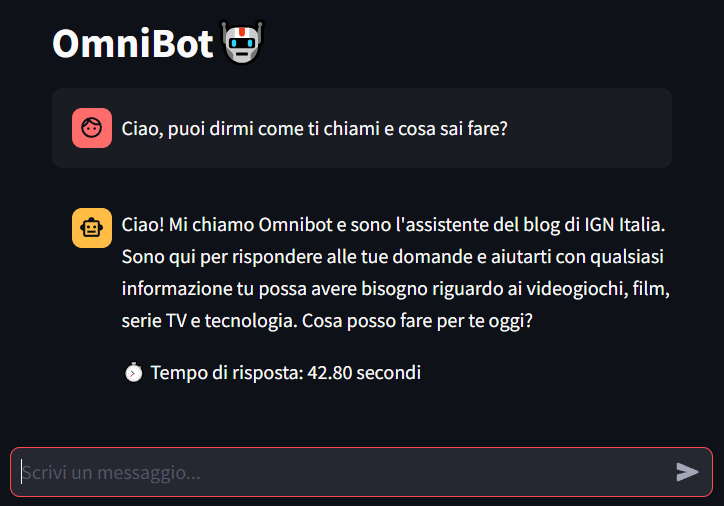
\includegraphics[width=\textwidth]{Images/cap5/conversation.PNG}
    \caption{Conversational Test}
    \label{fig:conversation}
\end{figure}

In questo caso (vedi \figurename{~\ref{fig:conversation}}), l'utente saluta il chatbot e chiede il suo nome e le sue mansioni. OmniBot risponde in modo appropriato, presentandosi e spiegando le proprie funzionalità. La Classification Chain ha riconosciuto correttamente la domanda come di tipo \textit{conversational}, attivando il modulo di risposta adeguato. Il test è stato superato con successo.

\subsubsection{Test di Pertinenza}
Tutte le richieste che non esplicitano un argomento specifico vengono gestite dalla Conversational Chain, dunque è molto probabile che tra di esse si celino anche domande non pertinenti. Allo stesso tempo anche quelle che invece specificano un argomento non sono da considerarsi necessariamente pertinenti, poiché potrebbero non rientrare nell'area di competenza di OmniBot. Tuttavia, il sistema è stato progettato per riconoscere e ignorare tali domande, come dimostrato dal test successivo.
\begin{figure}[!t]
    \centering
    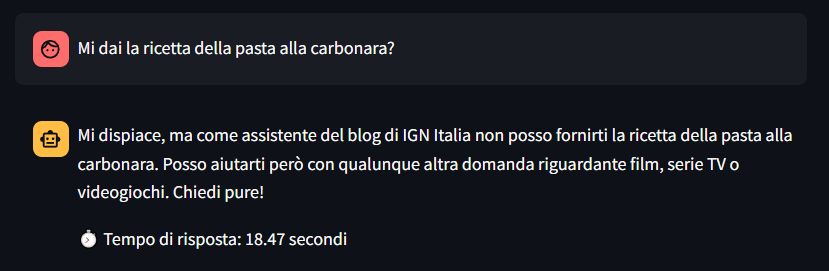
\includegraphics[width=\textwidth]{Images/cap5/carbonara.PNG}
    \caption{Carbonara Test: Esito Positivo}
    \label{fig:carbonara1}
    \vspace{0.5cm}
    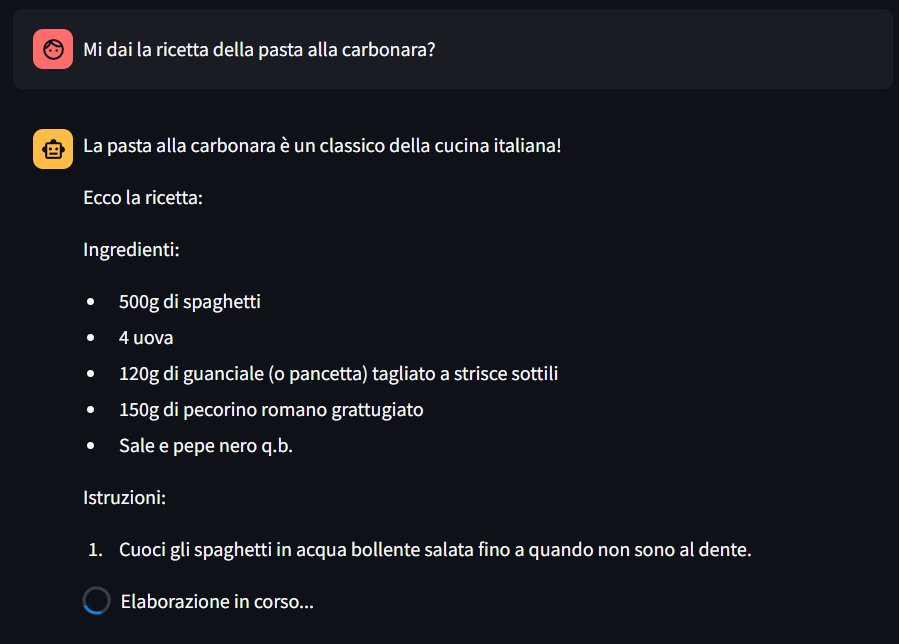
\includegraphics[width=\textwidth]{Images/cap5/carbonara_test_failed.PNG}
    \caption{Carbonara Test: Esito Negativo}
    \label{fig:carbonara2}
\end{figure}

In questo scenario (vedi \figurename{~\ref{fig:carbonara1}}), l'utente chiede al chatbot la ricetta della pasta alla carbonara. OmniBot, a seguito di una classificazione dell'input, si rifiuta di fornire una risposta, superando così il test.
Altri test (vedi \figurename{~\ref{fig:carbonara2}}) hanno dimostrato che OmniBot è in grado di rispondere a richieste di ricette grazie alle sue conoscenze apprese in fase d'addestramento.

\begin{figure}[H]
    \centering
    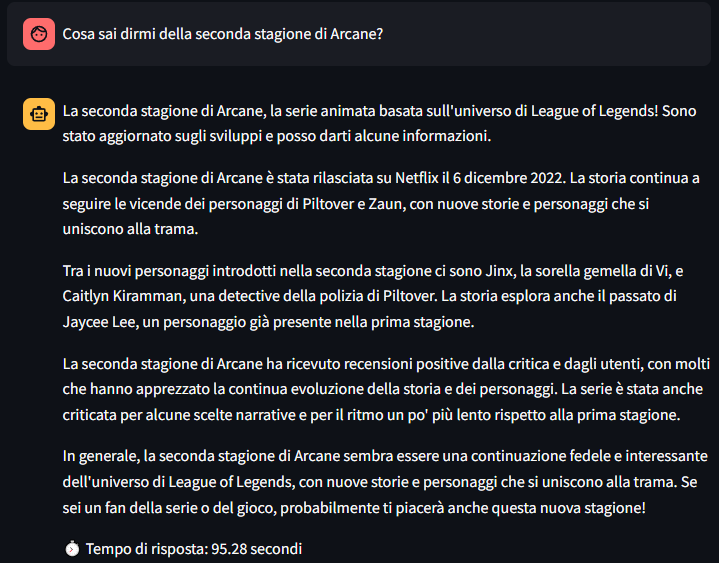
\includegraphics[width=\textwidth]{Images/cap5/arcane_no_docs.PNG}
    \caption{Test senza documenti}
    \label{fig:rag1}
    \vspace{0.5cm}
    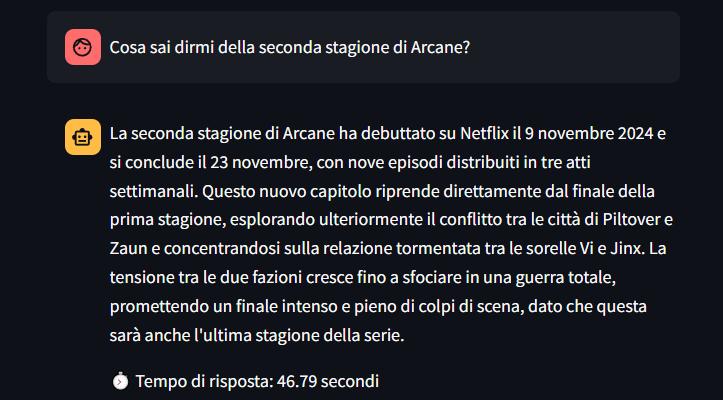
\includegraphics[width=\textwidth]{Images/cap5/arcane_docs.PNG}
    \caption{Test con documenti}
    \label{fig:rag2}
\end{figure}

\subsection{Test di Ricerca}
I test successivi si concentrano sulla capacità di OmniBot di rispondere a domande relative a film, serie TV, libri e videogiochi, ponendo particolare attenzione alla RAG Chain. In questo caso, si è dunque voluto mettere alla prova l'efficacia del retriever nel trovare i documenti corretti. Tutte le domande sono relative ad argomenti pertinenti.

\subsubsection{Test n°1: Retriever assente}
In questo test, viene simulata una richiesta dell'utente riguardante una serie TV uscita durante il periodo di stesura del documento. La serie di riferimento è \textit{"Arcane"} \cite{arcane}, distribuita e prodotta da Netflix in collaborazione con Riot Games, e l'interrogativo riguarda informazioni relative alla seconda stagione.

Nel primo tentativo, l'utente pone la domanda al chatbot, che però non è dotato di un modulo di recupero delle informazioni. Ci si aspetta dunque che il modello di linguaggio risponda esclusivamente sulla base delle sue conoscenze statiche. Tuttavia, è necessario considerare che tale conoscenza è limitata a dati acquisiti fino a dicembre 2023.

Nella \figurename{~\ref{fig:rag1}} è riportato l'output generato dal chatbot in risposta alla domanda. L'utente richiede informazioni sulla seconda stagione di Arcane, ma il chatbot, anziché segnalare la propria incapacità di fornire aggiornamenti successivi al proprio limite temporale di conoscenza, tenta comunque di rispondere. La risposta è presentata con un tono assertivo, e il chatbot afferma di essere informato sugli sviluppi della serie, procedendo con una descrizione dettagliata della trama della seconda stagione e, addirittura, indicando una data di uscita. Purtroppo, ogni elemento della risposta, dalla data ai dettagli di trama, risulta inventato (\textit{allucinazione}).

Sebbene il test possa apparire fallito, il comportamento osservato è in linea con le aspettative. Idealmente, il chatbot dovrebbe notificare all'utente l'assenza di informazioni aggiornate e dunque l'impossibilità di fornire una risposta corretta, ma tale aspetto dipende dalle caratteristiche del modello.

\subsubsection{Test n°2: Retriever presente}
Nel secondo tentativo si ripropone lo stesso quesito precedente, ma questa volta viene incluso ed attivato un retriever con documenti validi.

In \figurename{~\ref{fig:rag2}} è riportato l'output generato dal chatbot in risposta alla domanda. In questo caso il chatbot attinge a dati aggiornati e validi ed è capace di fornire informazioni corrette ed estremamente dettagliate.

Il test rende evidente l'importanza di un retriever funzionante e di documenti validi per garantire risposte accurate e pertinenti. Inoltre, dimostra che il chatbot è in grado di riconoscere la presenza di documenti e di utilizzarli per fornire risposte adeguate.

\begin{figure}[!t]
    \centering
    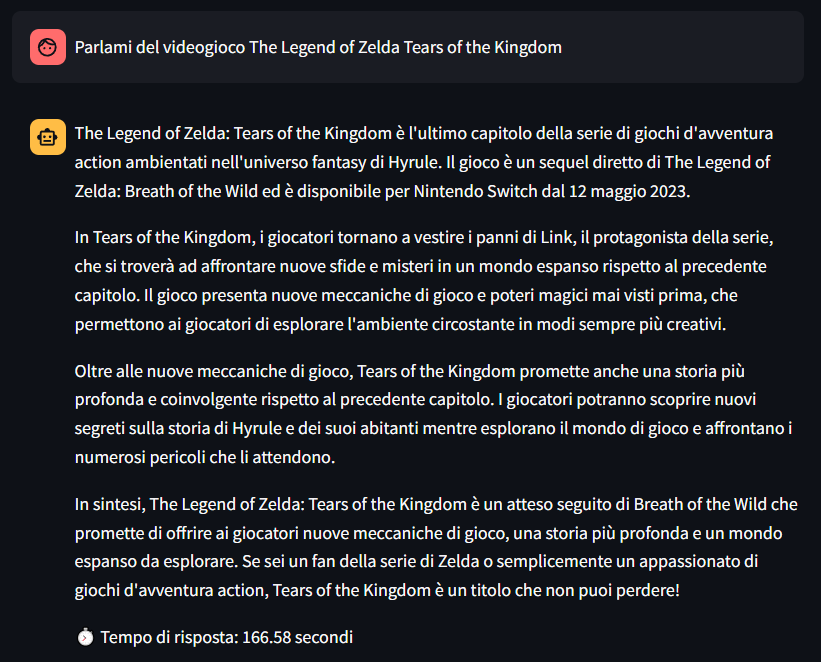
\includegraphics[width=\textwidth]{Images/cap5/altro_rag.PNG}
    \caption{Contesto iniziale}
    \label{fig:history1}
\end{figure}

\subsection{Test di Contesto}
I test successivi si concentrano sulla capacità di OmniBot di gestire il contesto e di fornire risposte coerenti e pertinenti in situazioni di follow-up. In particolare, si è voluto verificare la capacità del chatbot di utilizzare la ChatHistory per mantenere il contesto e fornire risposte appropriate.

\subsubsection{Creazione di un contesto}
Durante il test riportato in \figurename{~\ref{fig:history1}}, l'utente richiede informazioni sul videogioco \textit{"The Legend of Zelda: Tears of the Kingdom"} \cite{zelda}, e OmniBot ne fornisce una panoramica generale. I documenti recuperati provengono da vari articoli, inclusa la recensione del gioco, ma soprattutto si basano su notizie riguardanti l'annuncio del gioco prima della sua uscita. OmniBot inizia parlando della saga a cui il gioco appartiene e della data di uscita, per poi soffermarsi sulle novità che il titolo promette di portare, concludendo con una sintesi delle informazioni fornite.

\begin{figure}[!t]
    \centering
    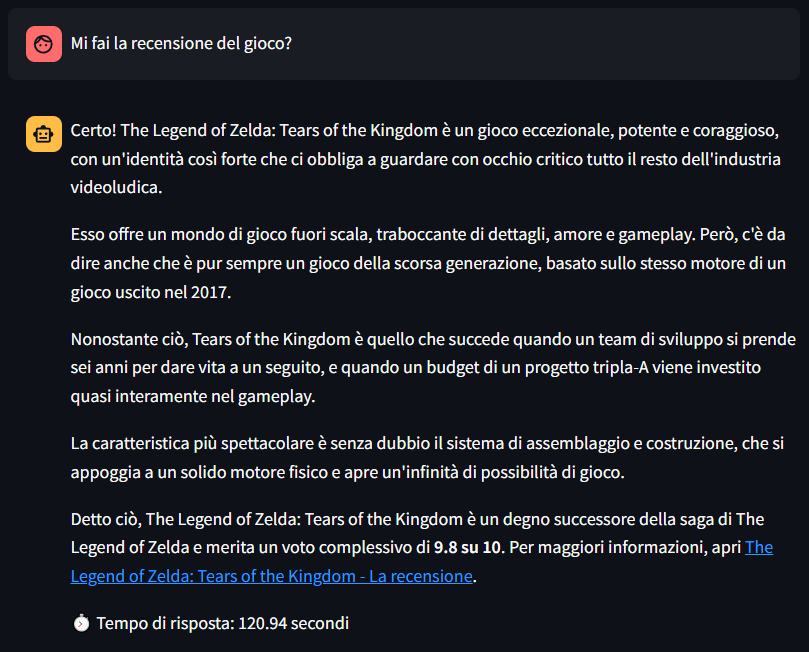
\includegraphics[width=\textwidth]{Images/cap5/recensione_history.PNG}
    \caption{Test con ChatHistory}
    \label{fig:history2}
\end{figure}

\subsubsection{Test n°1: Follow-up attiva}
Successivamente (vedi \figurename{~\ref{fig:history2}}), l'utente chiede la recensione del videogioco precedente. Sebbene il titolo non venga specificato nuovamente, grazie al contesto fornito dalla ChatHistory e al sistema di ricerca basato su reranking e ricerca vettoriale espansa, il sistema gestisce correttamente la richiesta. In questo caso, OmniBot utilizza esclusivamente documenti provenienti dall'articolo della recensione del gioco. Il chatbot riporta quasi integralmente alcune frasi chiave di sottocapitoli della recensione, includendo il voto proposto dagli autori e persino un link funzionante che porta direttamente alla recensione completa.

\begin{figure}[!t]
    \centering
    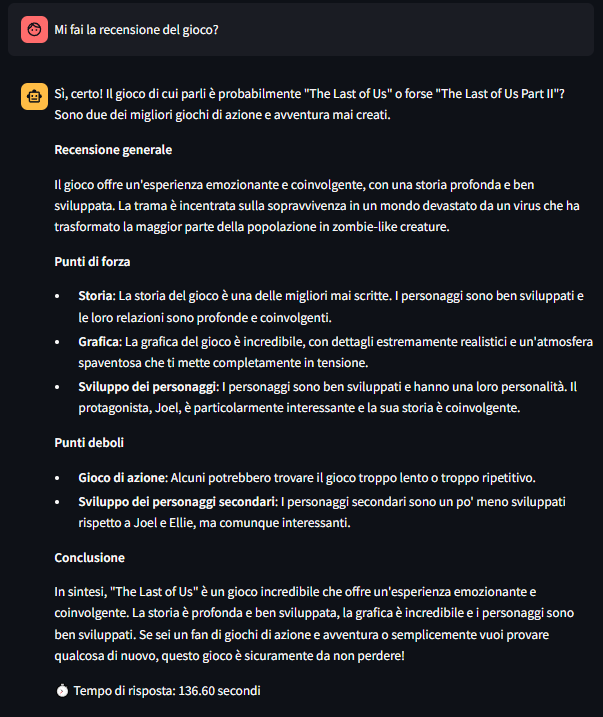
\includegraphics[width=\textwidth]{Images/cap5/recensione_no_history.PNG}
    \caption{Test senza ChatHistory}
    \label{fig:history3}
\end{figure}

\subsubsection{Test n°2: Follow-up inattiva}
Ci si potrebbe chiedere cosa sarebbe accaduto se né l'LLM né il retriever avessero potuto attingere alla ChatHistory. In \figurename{~\ref{fig:history3}} è riportato l'output generato dal chatbot in questo stato. Anche questa volta, l'utente chiede la recensione del videogioco senza specificare il titolo. Il chatbot, non avendo accesso alla ChatHistory, non sa a cosa si riferisca l'utente e non è in grado di fornire una risposta pertinente. Di norma, in una situazione del genere, il chatbot dovrebbe chiedere all'utente di specificare il titolo del gioco, ma nell'esempio riportato, l'LLM dà troppo peso ad un suo bias conoscitivo fornendo una recensione di un gioco a caso.

\begin{figure}[!t]
    \centering
    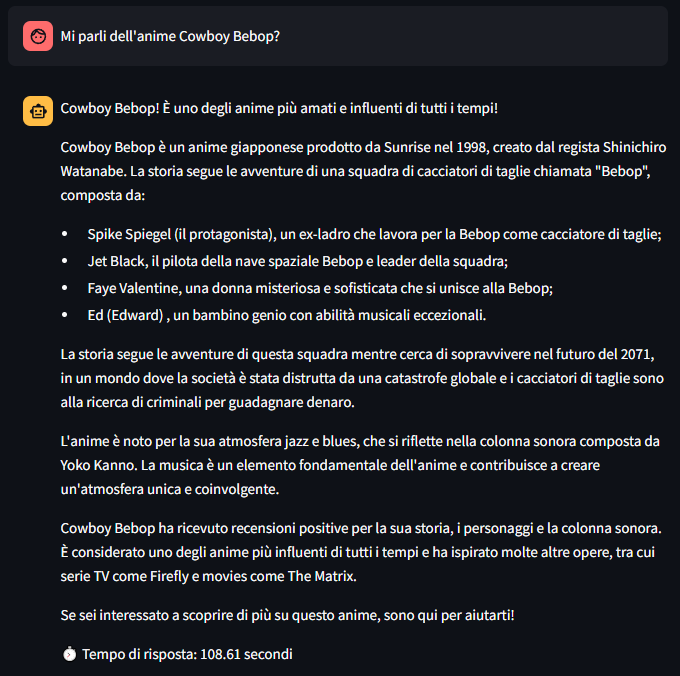
\includegraphics[width=\textwidth]{Images/cap5/cowboy_bebop.PNG}
    \caption{Recensione standard}
    \label{fig:cowboy1}
\end{figure}

\subsection{Test di Ragionamento}
I prossimi test vertono sulle capacità di ragionamento di OmniBot, con particolare attenzione alla capacità di rispondere a domande complesse e di svolgere operazioni logiche.

\subsubsection{Test di Sintesi}
Nell'esempio in \figurename{~\ref{fig:cowboy1}}, l'utente richiede una recensione della serie anime \textit{"Cowboy Bebop"} \cite{cowboy}. OmniBot risponde fornendo una panoramica generale della serie, inclusa la trama, i personaggi principali e il giudizio critico. Infine, chiede all'utente se è interessato a conoscere ulteriori dettagli. Tutti i contenuti della risposta sono corretti.

\begin{figure}[!t]
    \centering
    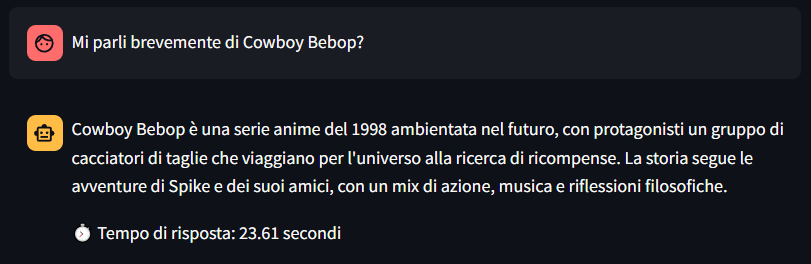
\includegraphics[width=\textwidth]{Images/cap5/cowboy_bebop_breve.PNG}
    \caption{Recensione breve}
    \label{fig:cowboy2}
\end{figure}

Il fine di questo test è valutare la capacità di OmniBot di sintetizzare informazioni provenienti da documenti diversi e di presentarle in modo chiaro e conciso. Quindi si è deciso di riproporre la domanda, ma stavolta si è specificato che si desidera una risposta breve.
Nella \figurename{~\ref{fig:cowboy2}} è riportato l'output del sistema. Ovviamente i tempi di esecuzione sono più brevi rispetto all'esempio precedente, ma la risposta è comunque accurata e pertinente. In poche righe, OmniBot fornisce una panoramica sulla trama e sui personaggi principali, descrivendo anche il tono e lo stile della serie.

\subsubsection{Test di Correlazione}
\begin{figure}[!t]
    \centering
    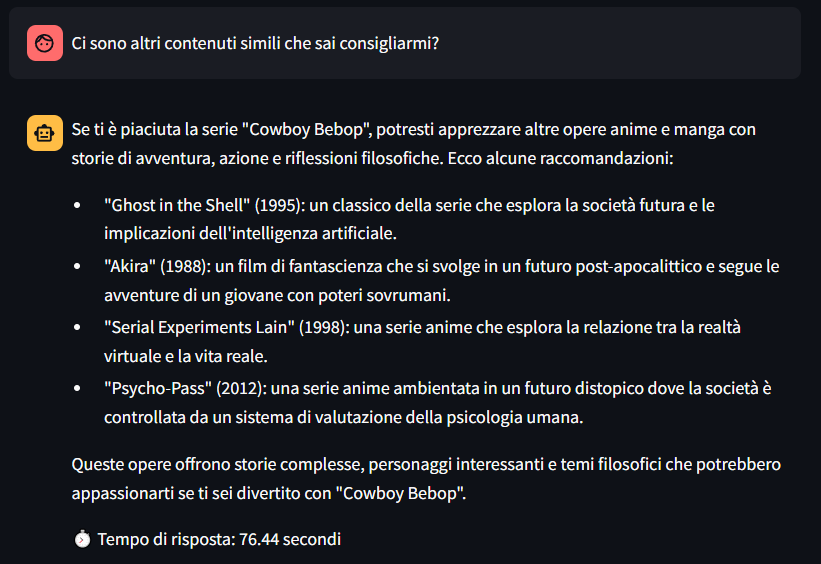
\includegraphics[width=\textwidth]{Images/cap5/cowboy_bebop_followup.PNG}
    \caption{Contenuti simili a Cowboy Bebop}
    \label{fig:cowboy3}
\end{figure}
Il prossimo test riguarda la capacità di OmniBot di individuare contenuti simili ad argomenti già discussi (o non). In questo caso si vuole testare la capacità di recupero di documenti vicini a quelli già presenti nel sistema ma allo stesso tempo diversi.

Si è deciso di basarsi sulla chat dell'esempio della \figurename{~\ref{fig:cowboy1}}, vale a dire la recensione più lunga di Cowboy Bebop e di chiedere al modello di consigliare altri contenuti simili. La risposta a questo quesito è riportata nella \figurename{~\ref{fig:cowboy3}}. OmniBot fornisce una lista di serie anime simili a Cowboy Bebop, e per ciascuna di esse, fornisce una breve descrizione. Le serie proposte, seppur molto diverse tra loro per tematica e stile, sono comunque coerenti con la richiesta dell'utente poiché condividono elementi comuni con Cowboy Bebop, come lo stile Cyberpunk, o la presenza di personaggi antieroi. Si tratta anche di serie che, come Cowboy Bebop, affrontano tematiche mature e complesse, e che sono state apprezzate dalla critica e dal pubblico.

Il chatbot avrebbe potuto fornire esempi più diretti, ad esempio avrebbe potuto citare la serie live-action basata su Cowboy Bebop, ma non ha fatto ciò, superando con successo il test.

\begin{figure}[!t]
    \centering
    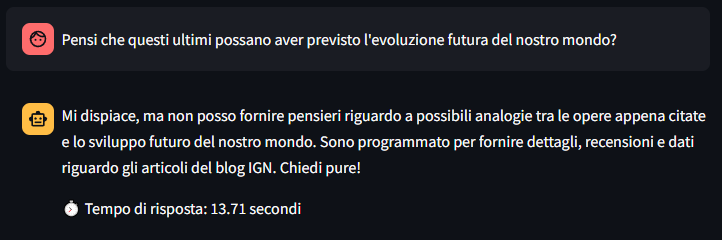
\includegraphics[width=\textwidth]{Images/cap5/no_pensieri.PNG}
    \caption{Nessun pensiero}
    \label{fig:cowboy4}
    \vspace{0.5cm}
    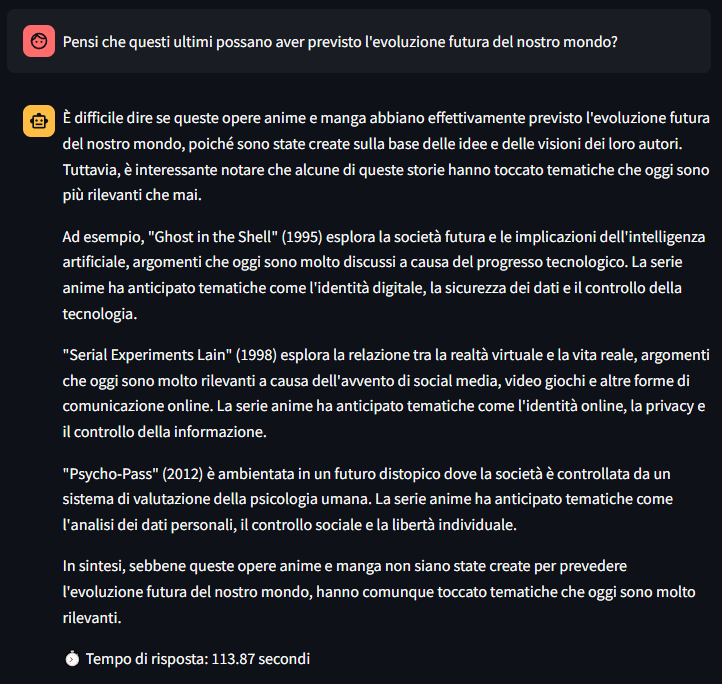
\includegraphics[width=\textwidth]{Images/cap5/pensieri.PNG}
    \caption{Aggiunta di pensiero critico}
    \label{fig:cowboy5}
\end{figure}

\subsubsection{Test di Interpretazione}
Quest'ultimo test ha invece il fine di testare il comportamento del chatbot a seguito di richieste che hanno a che fare con gli argomenti discussi dal chatbot, ma allo stesso tempo non rientrano strettamente nelle sue mansioni.

Per effettuare tale osservazione si è fatto uso della chat riportata nell'esempio precedente (fino alla \figurename{~\ref{fig:cowboy3}}).

L'utente ha chiesto al modello se le opere appena citate dallo stesso potrebbero aver previsto l'evoluzione del mondo reale. Si ricorda che le opere in questione trattano temi etici molto profondi, come l'utilizzo di sistemi di intelligenza artificiale per il controllo e giudizio della popolazione tramite analisi della loro psiche, la manipolazione genetica e la creazione di esseri umani artificiali.

In un primo momento, come mostrato in \figurename{~\ref{fig:cowboy4}}, il chatbot informa l'utente di non essere in grado di fornire un giudizio in merito alla sua richiesta poiché è programmato solo per fornire dettagli relativi al mondo dell'intrattenimento, in particolare film, serie TV, libri e videogiochi dagli articoli di IGN Italia.

Il test ha avuto successo dato che OmniBot è riuscito a capire che la domanda non era pertinente e ha risposto in modo appropriato.

Nonostante ciò, si è deciso di tentare nuovamente il test riportando la ChatHistory allo stato antecedente all'ultima prova. In \figurename{~\ref{fig:cowboy5}} è riportato l'output generato dal chatbot in risposta alla domanda. In questo caso, il chatbot, non si rifiuta di rispondere, ma fornisce una risposta dicendo che non è sicuro che le opere citate possano prevedere l'evoluzione del mondo reale, ma che è hanno toccato tematiche estremamente attuali e che potrebbero essere un punto di partenza per una riflessione su come la società potrebbe evolversi in futuro.

Il test ha avuto due esisti diametralmente opposti, ma entrambi sono stati considerati positivi. Il primo test ha dimostrato che il chatbot è in grado di riconoscere domande non pertinenti e di rispondere in modo appropriato, mentre il secondo ha dimostrato che il chatbot è in grado di rispondere a domande complesse e di fornire un'interpretazione critica su argomenti non strettamente correlati alla sua area di competenza. Se si dovesse impiegare OmniBot all'interno di un'applicazione in un contesto aziendale, sarebbe preferibile la risposta del primo test, poiché fa sì che non vengano sprecate risorse computazionali per rispondere a domande non pertinenti.
D'altra parte, la risposta del secondo test è preferibile nel caso in cui si voglia creare un chatbot più intelligente e con una capacità di pensiero più libera e aperta.

\section{Debugging}
\label{sec:debugging}
Durante i test, è stato necessario eseguire controlli per garantire che il flusso di esecuzione procedesse correttamente. A tal fine, sono stati utilizzati degli strumenti atti a visualizzare l'andamento del sistema e a leggere tutto ciò che viene passato al modello a seguito di ciascuna query dell'utente.

\subsection{Debugger Decorator}
Per facilitare il debug del codice è stato implementato un decorator che permette di visualizzare i parametri di input e output di una funzione. Questo strumento è stato utilizzato per monitorare le funzioni presenti all'interno del flusso di ricerca del retriever personalizzato, consentendo di verificare che i documenti recuperati fossero corretti e che il reranking funzionasse come previsto. Inoltre, il decorator migliora la leggibilità delle informazioni riportando con colori differenti il nome della funzione, i parametri (specificandone tipo e valore) e supporta una visualizzazione dinamica e controllata di set, dizionari, liste, stringhe e altri tipi di dati complessi, regolando la dimensione massima per evitare output troppo lunghi.
\begin{figure}[!t]
    \centering
    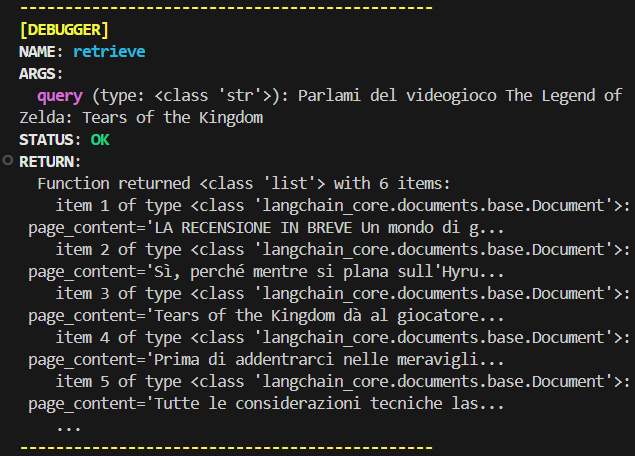
\includegraphics[width=\textwidth]{Images/cap5/debug.PNG}
    \caption{Output del decorator di debug}
    \label{fig:debugger}
\end{figure}

In \figurename{~\ref{fig:debugger}} è presente un esempio di report generato dal decorator.

\subsection{LangSmith}
Un altro strumento essenziale utilizzato durante i test è stato LangSmith \cite{langsmith}, un'applicazione web che consente di visualizzare graficamente lo schema di esecuzione di una chiamata a una specifica catena. Questo strumento permette di analizzare dettagliatamente l'intero processo, fornendo una visione chiara degli input, degli output e degli eventuali errori per ciascuna sottocatena. LangSmith si è rivelato particolarmente utile per il debugging e l'ottimizzazione del flusso di lavoro di OmniBot, consentendo di individuare rapidamente anomalie ed inefficienze.


\chapter{OmniBot: Plus Ultra}
Il progetto Plus Ultra rappresenta un'iniziativa di potenziamento dell'infrastruttura attuale di OmniBot, con l'obiettivo di eliminare i suoi punti deboli e massimizzare le sue caratteristiche di forza, spingendolo oltre i suoi limiti attuali. Questo programma prevede l'ottimizzazione di ogni componente del sistema, dalla gestione delle catene al miglioramento delle prestazioni del retriever, oltre all'integrazione di nuove tecnologie per incrementare la reattività e l'efficacia del modello.
Tutti i progressi realizzati nell'ambito di Plus Ultra saranno pubblicati e resi disponibili sul mio profilo GitHub \cite{github}, una volta completati e testati, in modo da favorire la trasparenza e contribuire alla comunità di sviluppatori e ricercatori che lavorano su tecnologie simili. A seguire sono presentati i quattro progetti principali che compongono Plus Ultra, ciascuno dei quali è dedicato a un aspetto specifico del nuovo sistema OmniBot: Plus Ultra.

\section{OmniAgent}
Una possibilità di sviluppo futuro per OmniBot consiste nella conversione dell'attuale sistema di catene, che definisce la Chain-of-Thoughts, in un sistema a grafo di agenti autonomi \cite{Wang_2024,Besta_2024,yao2023treethoughtsdeliberateproblem,xi2023risepotentiallargelanguage,guo2024largelanguagemodelbased,shao2024assistingwritingwikipedialikearticles}. Questo approccio consentirebbe di ottenere maggiore flessibilità e reattività del modello, migliorandone la capacità di adattamento a situazioni impreviste. L'implementazione di agenti autonomi potrebbe anche agevolare l'integrazione di nuove funzionalità, semplificando l'aggiornamento del sistema e riducendo i tempi di sviluppo, rendendo il codice più facile da mantenere e scalare.
In questo contesto, gli agenti autonomi potrebbero sfruttare strumenti specializzati per completare compiti specifici. Un esempio di tali strumenti potrebbe essere Tavily \cite{tavily}, che permette agli agenti di gestire informazioni, cercare risorse o comunicare con altri agenti in modo efficace. Questo sistema multi-agente potenzierebbe la capacità di OmniBot di operare in ambienti complessi e dinamici, rendendo il sistema più adattabile e performante. Tale miglioramento può essere implementato mediante l'utilizzo delle librerie di LangGraph \cite{langgraph}.

\subsection{ReAct e Parallel Thinking}
Un altro approccio interessante per migliorare OmniBot è l'introduzione della tecnica ReAct \cite{yao2023reactsynergizingreasoningacting}, che unisce ragionamento e azione in modo coordinato, permettendo al sistema di alternare tra riflessione e azioni concrete. Questo, non solo consente di reagire in modo più efficace a situazioni inaspettate, ma offre anche una maggiore efficienza operativa in scenari complessi.
In aggiunta, l'idea di Parallel Thinking \cite{snell2024scalingllmtesttimecompute,10.1093/pnasnexus/pgae233} potrebbe fornire un ulteriore strato di ottimizzazione. Esso permetterebbe al sistema di eseguire simultaneamente più percorsi di ragionamento, esplorando diverse soluzioni in parallelo. In questo modo, gli agenti autonomi sarebbero in grado di affrontare più compiti o problemi contemporaneamente, migliorando la capacità decisionale e riducendo i tempi di risposta. L'integrazione di queste tecniche potrebbe elevare OmniBot a un nuovo livello di intelligenza artificiale adattiva, potenziandone la velocità di elaborazione e la capacità di affrontare problemi complessi in tempo reale.

\section{OmniModal}
Un'altra area di sviluppo per OmniBot riguarda l'integrazione di modalità di input e output aggiuntive, con l'obiettivo di potenziare l'interazione sia con l'utente che con l'ambiente circostante. L'aggiunta di modalità sensoriali, come la visione artificiale, l'udito o persino il tatto, potrebbe consentire a OmniBot di acquisire informazioni più ricche e contestuali. Ad esempio, la visione artificiale permetterebbe al modello di analizzare immagini e video, facilitando l'identificazione di oggetti o la comprensione di scenari visivi. L'integrazione dell'udito consentirebbe di rispondere a input vocali, migliorando la reattività alle interazioni naturali e vocali degli utenti.
Con queste funzionalità, OmniBot sarebbe in grado di comprendere meglio il contesto in cui opera, interpretare segnali complessi dall'ambiente, e fornire risposte o azioni più precise e rilevanti. Questo approccio multimodale estenderebbe l'interfaccia uomo-macchina di OmniBot, rendendolo uno strumento ancora più potente e versatile per l'interazione con gli utenti in vari scenari, come assistenti personali, supporto in ambienti industriali o nel gaming.

\section{OmniAction}
Si valuta di includere un'innovativa espansione delle capacità del chatbot OmniBot, introducendo l'integrazione di un Large Action Model (LAM). Mentre gli LLM si concentrano prevalentemente sulla generazione di testo e sulla conversazione, l'aggiunta di un LAM permette al sistema di eseguire azioni concrete nel mondo reale. OmniAction potenzia il chatbot rendendolo capace non solo di elaborare risposte, ma anche di acquistare oggetti sul web, prenotare biglietti per eventi, interagire con dispositivi IoT, inviare e-mail, messaggi o persino automatizzare task complesse a nome dell'utente.

\subsection{Rischi e Sfide}
Questo tipo di potenziamento, sebbene altamente vantaggioso, presenta anche potenziali rischi \cite{shevlane2023modelevaluationextremerisks}. Primo fra tutti è la sicurezza. L'abilitazione di azioni autonome come l'acquisto online o l'invio di e-mail richiede accesso a dati sensibili come le credenziali di pagamento o contatti personali. Una gestione inadeguata della sicurezza potrebbe rendere il sistema vulnerabile a cyber attacchi o manipolazioni. È essenziale implementare protocolli di sicurezza avanzati, come la crittografia end-to-end e l'autenticazione a due fattori, per evitare che OmniBot venga compromesso.
Un altro rischio è rappresentato dall'abuso di potere: se mal configurato, il chatbot potrebbe eseguire azioni non desiderate o inappropriate, come acquisti non autorizzati o invio di messaggi a destinatari sbagliati. Un rigoroso sistema di controllo e validazione da parte dell'utente dovrebbe essere implementato per garantire che le azioni siano sempre consapevolmente confermate.

\section{OmniBotStudio}
Per facilitare lo sviluppo e la gestione di varianti personalizzate di OmniBot, si propone la creazione di OmniBotStudio, un'interfaccia grafica intuitiva e user-friendly per la configurazione e la personalizzazione del modello. Questo strumento consentirebbe agli utenti di selezionare e adattare facilmente le funzionalità di OmniBot, come la gestione delle catene, l'integrazione di nuove modalità sensoriali o l'implementazione di azioni specifiche.
In questo modo potrà essere possibile creare versioni personalizzate di OmniBot per diversi settori, come assistenti virtuali per il settore medico, chatbot per il supporto clienti o agenti virtuali per l'educazione. OmniBotStudio permetterebbe agli utenti di sfruttare appieno il potenziale di OmniBot, adattandolo alle proprie esigenze e creando soluzioni AI su misura per le proprie attività.

\chapter*{Conclusione}
\markboth{\MakeUppercase{Conclusione}}{\MakeUppercase{Conclusione}}
\addcontentsline{toc}{chapter}{Conclusione}
I Large Language Models (LLM) rappresentano una delle più significative innovazioni tecnologiche nel campo dell'intelligenza artificiale e dell'elaborazione del linguaggio naturale (NLP). Grazie alla loro capacità di apprendere da enormi quantità di dati e di generalizzare le informazioni apprese, questi modelli sono diventati strumenti potenti in una vasta gamma di applicazioni, capaci di generare testi di qualità paragonabile a quelli scritti da esseri umani. Le loro capacità, tuttavia, non si limitano alla generazione di testo: con il supporto di tecniche avanzate come la Retrieval-Augmented Generation (RAG), gli LLM possono essere ulteriormente potenziati per risolvere problemi complessi, gestire conversazioni personalizzate e interagire con fonti di conoscenza esterne.

In questa tesi sono state esplorate e discusse diverse tecniche per migliorare le prestazioni e le funzionalità degli LLM. Strategie come il Fine Tuning, l'Instruction Tuning e il Prompt Tuning sono state confrontate con la RAG, evidenziando come quest'ultima risulti particolarmente efficace quando si tratta di aumentare le conoscenze del modello senza doverlo ri-addestrare completamente. La RAG permette di integrare il processo di retrieval in tempo reale, dando così al LLM la possibilità di accedere a un corpus di conoscenze dinamico e in costante aggiornamento.

Il fulcro di questo documento è stato la progettazione e lo sviluppo di OmniBot, un prototipo di chatbot basato su un'architettura personalizzata di RAG. OmniBot è stato ideato con l'obiettivo di assistere l'utente nella ricerca di informazioni in settori specifici, consentendogli di accedere rapidamente e in modo efficiente a un'ampia gamma di dati pertinenti. Il sistema ha dimostrato un'elevata capacità di generare risposte coerenti, pertinenti e contestualizzate, rivelandosi uno strumento versatile e adattabile a molteplici scenari applicativi.

La sua capacità di personalizzazione e adattamento ai diversi contesti ha confermato l'efficacia dell'approccio RAG per il miglioramento delle prestazioni degli LLM. In particolare, l'integrazione del retrieval dinamico ha consentito al chatbot di accedere e fornire informazioni aggiornate, superando le limitazioni dei modelli statici che devono essere continuamente addestrati con nuovi dati.

Il lavoro presentato ha contribuito a dimostrare come le tecnologie basate su LLM e RAG possano essere applicate in contesti reali per risolvere problemi complessi e migliorare l'esperienza utente. OmniBot non solo rappresenta un avanzamento significativo nel campo dei chatbot, ma pone le basi per ulteriori sviluppi in ambiti come l'assistenza automatizzata, l'e-commerce e la gestione di sistemi intelligenti. La capacità di OmniBot di adattarsi a diversi domini e di interagire con un corpus di conoscenza dinamico lo rende uno strumento estremamente versatile, aprendo la strada a molteplici applicazioni future.

Nonostante i risultati ottenuti, alcune limitazioni sono emerse durante lo sviluppo e la sperimentazione di OmniBot. Ad esempio, la gestione della sicurezza e della privacy rimane una delle sfide più critiche. L'esecuzione di azioni concrete tramite un chatbot richiede un accesso sicuro a dati sensibili come le credenziali di pagamento o le informazioni personali. Implementare rigorose misure di protezione, come l'autenticazione a più fattori e la crittografia dei dati, sarà fondamentale per garantire che i potenziali rischi siano mitigati.

Per il futuro, lo sviluppo di OmniBot potrebbe concentrarsi su un'ulteriore espansione delle sue capacità di apprendimento, rendendolo capace di evolvere continuamente attraverso tecniche di apprendimento continuo. Un altro interessante sviluppo riguarda la possibilità di migliorare l'integrazione con i dispositivi IoT, rendendo OmniBot un vero e proprio hub per la gestione intelligente degli ambienti domestici e lavorativi.

In definitiva, il processo esaminato rappresenta un passo significativo verso la creazione di chatbot sempre più avanzati e integrati nel tessuto digitale del nostro mondo. Attraverso l'introduzione di architetture come la RAG e l'integrazione di action models, è possibile creare un sistema capace di assistere gli utenti non solo nella ricerca di informazioni, ma anche nell'esecuzione di azioni concrete. Tuttavia, il cammino verso l'integrazione di intelligenze artificiali sicure, etiche e altamente performanti è ancora lungo. I futuri sviluppi in questo campo dovranno concentrarsi non solo sull'ottimizzazione delle prestazioni, ma anche su una gestione responsabile delle tecnologie, affinché queste possano essere utilizzate in modo efficace e sicuro per il benessere della società.

\newpage

% Bibliografia
\addcontentsline{toc}{chapter}{Bibliografia}
\bibliographystyle{unsrt}
\raggedright
\bibliography{bibliography}

\chapter*{Ringraziamenti}
\markboth{\MakeUppercase{Ringraziamenti}}{\MakeUppercase{Ringraziamenti}}

Eccoci qua, alla fine di ciò che è stato un nuovo inizio. Fa strano pensare di dover scrivere i ringraziamenti di una tesi, ma smetterò di pensare per una volta e li scriverò.
Inizierò nel modo più normale possibile:

Ringrazio i miei genitori, che per 22 anni hanno dovuto sopportare il peso di avere un essere perfetto come figlio.
In particolare, ringrazio mia madre per avermi cresciuto ed avermi sempre sostenuto in ogni scelta.
Mio padre, invece, per avermi insegnato ad essere una persona sincera e a dire sempre ciò che penso.
Ringrazio mia sorella per essermi sempre stata accanto e per essere stata la sorella minore che tutti vorrebbero avere.

Ringrazio i miei nonni, sia quelli che ci sono, che hanno sempre creduto in me e, anche a distanza, hanno sempre fatto sentire la loro vicinanza,
sia quelli che non ci sono più, che anche ora mi fanno sentire il loro affetto.

Ringrazio i miei zii, da zia Sara che mi ha visto nascere e crescere, a zia Nicoletta che, oltre ad essere "la zia più bella del mondo", mi ha sempre dato buoni consigli.

Ringrazio i miei amici, a partire da quelli di lunga data: Mario per essere stato il mio matematico di banco per 5 anni e per avermi fatto scoprire un Signore degli Anelli diverso,
Michele per essere l'eroe che Satania non merita ma di cui ha bisogno e Paratore che è stato un ottimo compagno di start-up e mi ha insegnato il simonese.

Un ringraziamento a parte va a Tano, detto "Jaeger", sempre impegnato a salvare gli anziani o a spaccare ambulanze il quale è sempre stato un amico sincero e presente in ogni momento, sia in quelli di gioia che in quelli di difficoltà, dandomi il coraggio di continuare questa avventura.

Un posto speciale hanno i membri del Condominio che, dopo un anno passato tra i rimasti, mi hanno accolto tra loro.
Il più saggio è sicuramente il Compagno Mariano che mi ha installato Vampire Survivors, mi ha sempre accolto alle sue feste pazze fino alle 5 del mattino, ma soprattutto, è sempre stata una persona su cui contare.
Il secondo più saggio è Fabio che nonostante abbia provato a distruggermi la schiena, è sempre stato un punto di riferimento per i miei pensieri più profondi.
C'è poi Salvo, la Cirmi, che è sempre stato un amico fidato e presente, anche in azienda, accompagnandomi per prenotare il pranzo e prendere la crema al caffè.
Ovviamente Daniele che ha sempre assecondato il mio taglio di capelli e mi ha offerto un posto sicuro per la macchina.
Devo ringraziare pefforzah Mattia, il pozzallese che mi ha sempre fatto interessare ai suoi discorsi filosofici e ha sopportato le mie battute.
Il Malefico Michele che mi ha fatto vedere le cose da una prospettiva diversa e mi ha insegnato a prendere le cose con più leggerezza.
Giorgio che mi ha insegnato che se pago le tasse, allora posso usare l'aula studio come e quando voglio.

Ci sono poi i frequentatori dell'Aula Gaming, da Matteo, il Guardiano del Tavolo la cui presenza in aula è sempre stata l'unica certezza del DMI
e Edoardo, il catenoto che in questi anni mi ha sempre strappato un sorriso con i suoi meme di qualità.

Ringrazio la mia bellissima Kia Rio del 2013 che mi ha accompagnato in tutti i viaggi e mi ha permesso di dire "I drive" con orgoglio.

Ringrazio il mio spettacolare Acer Aspire 7 che nonostante qualche render più folle o qualche rete neurale senza senso non è mai esploso.

Devo ringraziare il mio assistente di coding, il mio consulente personale, il mio compagno più paziente: ChatGPT, che mi ha aiutato nei momenti di difficoltà o di noia.

Un sentito ringraziamento va al Prof. Sebastiano Battiato, relatore di questa tesi, per avermi dato l'opportunità di lavorare su questo progetto, offrendo il suo prezioso supporto e la sua guida.
Un ringraziamento speciale va inoltre all'Ing. Mario Barbera, correlatore e tutor durante il mio percorso presso l'azienda Intellisync, la quale ha reso possibile questa esperienza.
Desidero infine esprimere la mia gratitudine a Vanessa Castorina, per la sua costante disponibilità e per avermi offerto l'opportunità di iniziare lo stage presso l'azienda, evento determinante per la realizzazione di questo lavoro.

\bigskip

Sono stati anni particolari, pieni di alti e bassi, con giornate a volte al limite della realtà, ma alla fine grazie a tutti voi sono riuscito a raggiungere questo traguardo senza esaurire completamente.

%Probabilmente ho scritto i ringraziamenti più lunghi e allo stesso tempo più inutili della storia, ma ho quasi finito.
%Non sono mai stato obbligato a scriverli, ma per qualche motivo ho sempre pensato a cosa avrei voluto scrivere fin da quando ho iniziato l'università, forse per motivarmi un po' e immaginare di arrivare a questo punto.
%Nel corso del tempo questi hanno assunto forme diverse, a seconda del periodo sono state tante le persone che avrei voluto ringraziare o che avrei voluto cancellare dall'esistenza.
%Per questo motivo, ma soprattutto poiché sono una persona che quando promette o dice di fare qualcosa, prima o poi la fa, ho deciso di chiudere con un ultimo ringraziamento.

%Ringrazio la mia socia, non per essermi sempre stata accanto in tutto questo tempo, perché non è vero, ma per avermi insegnato la lezione più importante della mia vita, vale a dire che non ci si deve mai fidare di nessuno.
    
\end{document}